\chapter{物理信息驱动的神经网络方法求解反势能问题}
在前一章中，我们详细探讨了利用深度里兹法（Deep Ritz Method）求解正向的椭圆型多特征值问题。沿着偏微分方程数值解的脉络，本章将视点转向一类更具挑战性、且在实际工程中极为重要的逆问题（Inverse Problems）：即在已知部分边界或内部测量数据的前提下，反向推演系统方程中的未知物理参数。具体而言，我们将提出并分析一种基于物理信息神经网络（PINNs）结合 Tikhonov 正则化的高效求解框架，用于重构椭圆方程中的未知势函数。
\section{预备知识与记号}
\subsection{问题背景与物理意义}

本文所研究的带有未知势函数的椭圆型偏微分方程在自然科学与工程领域具有极其广泛的物理背景。在宏观尺度上，此类方程常用于描述与时间无关的扩散现象或稳态热传导过程。例如，在定态扩散方程中 \cite{Bal2010Inverse}，未知的势函数通常对应于介质中的吸收（或反应）系数；而在稳态热传导模型中，它则代表了材料内部的辐射系数 \cite{Chen2020Convergence}。在微观尺度上，该类方程在形式上等价于定态薛定谔（Schrödinger）方程，用于描述微观粒子在特定势场中的量子态行为，此时未知项即对应于系统所处的势能分布。

在上述实际应用场景中，系统的内部参数（即势函数）往往无法被直接观测或先验给定。相反，我们通常只能通过传感器获取整个物理区域内部或其边界上的状态变量（如温度、浓度、波函数幅值等）的含噪测量值。因此，如何从这些不完全且带有噪声的观测数据中稳定、高精度地反演重构出真实的势函数，构成了典型的反问题。这类反势能问题在医学成像（如光学相干断层扫描）、地球物理勘探以及材料无损检测等领域具有不可替代的核心应用价值。

\subsection{数学描述与问题假设}
基于上述物理背景，我们将该反问题抽象为如下数学模型。我们考虑如下带有 Neumann 边界条件的椭圆型边值问题：
\begin{equation}\label{eq:pde:potential}
\left\{
\begin{aligned}
-\nabla\cdot(\alpha\nabla u)+Vu&=g, \quad \text{在}~\Omega~\text{中},\\
\alpha&=h, \quad \text{在}~\partial\Omega~\text{上},
\end{aligned}
\right.
\end{equation}
其中，$\Omega \subset \mathbb{R}^{d}$ 是给定的物理区域，$\alpha$ 为传导系数，$g$ 为内部源项，$h$ 为边界通量，$\partial_{\nu}$ 表示沿单位外法向量的导数。
给定一个确定的势函数 $V \in \mathcal{K}$，根据经典的椭圆偏微分方程理论 \cite{evans2010partial}，方程 \eqref{eq:pde:potential} 存在唯一的弱解 $u_V\in H^{1}(\Omega)$。基于此，我们可以良定义一个从参数空间到状态空间的非线性正演算子（Forward Operator）：
$$\mathcal{F}: V \mapsto u_V$$
为确保偏微分方程的适定性（Well-posedness）以及后续反问题理论分析的严密性，我们对计算区域和已知函数提出如下基本假设：

\begin{assumption}[正则性与有界性假设]\label{ass:tikpinn}
假设区域 $\Omega$ 和方程参数满足如下条件：
\begin{enumerate}
\item[(a)] 区域 $\Omega\subset\mathbb{R}^{d}$ ($d\geq1$) 为具有足够光滑边界 $\partial\Omega$ 的有界连通区域。传导系数 $\alpha\in C^{1}(\bar{\Omega})$，且满足一致椭圆条件：即存在常数 $\alpha_0>0$，使得对所有 $x\in\bar{\Omega}$ 均有 $\alpha(x)\geq\alpha_0$ 成立。
\item[(b)] 源密度函数满足 $g\in L^{2}(\Omega)$，边界通量函数满足 $h\in L^{2}(\partial\Omega)$。
\item[(c)] 真实的势函数 $V$ 属于如下有界容许集（Admissible Set）：
\begin{equation}\label{eq:box}
\mathcal{K}=\{V\in L^{\infty}(\Omega):0\leq\underline{V}\leq V(x)\leq\overline{V}<\infty,~\text{a.e. } x\in\Omega\},
\end{equation}
其中常数 $\underline{V}$ 和 $\overline{V}$ 分别代表容许势函数 $V(x)$ 的先验全局下界和上界。
\end{enumerate}
\end{assumption}

在反问题的设定下，我们的目标是利用状态变量 $u$ 的观测数据来重构真实的势函数 $V^\dagger \in \mathcal{K}$。在现实物理实验中，传感器采集的数据不可避免地会受到噪声污染。在整篇文章中，我们假设含噪测量数据服从如下标准的高斯加性噪声模型：
\begin{equation}\label{eq:measurement}
\left\{
\begin{array}{rcll}
u^{\delta}(x)&=&\mathcal{F}(V^{\dagger})(x)+\varepsilon_{\calI}(x),\quad &\varepsilon_{\calI}(x)\sim N(0,\delta^{2}),\quad x\in\Omega, \\ 
Tu^{\delta}(x)&=&T\mathcal{F}(V^{\dagger})(x)+\varepsilon_{\calB}(x),\quad &\varepsilon_{\calB}(x)\sim N(0,\delta^{2}),\quad x\in\partial\Omega,
\end{array}
\right.
\end{equation}
其中，$\delta > 0$ 表示噪声水平（Noise Level），$T$ 是经典的边界迹算子（Trace Operator）。基于上述统计模型，在 $L^2$ 范数意义下，含噪数据与真实状态之间满足如下确定性误差估计：

$$\|u^{\delta}-\mathcal{F}(V^{\dagger})\|_{L^{2}(\Omega)}=|\Omega|^{1/2}\delta, \quad \|Tu^{\delta}-T\mathcal{F}(V^{\dagger})\|_{L^{2}(\partial\Omega)}=|\partial\Omega|^{1/2}\delta.$$

\section{重构方法：Tikhonov-PINNs}\label{sec:tikpinns}
基于前述的数学模型，反问题的核心在于寻找一个势函数 $V$，使得其对应的系统正向响应 $u_V = \mathcal{F}(V)$ 尽可能逼近实际的测量数据。为此，我们首先定义如下的数据失配项（Data Mismatch）或测量误差泛函：
\begin{equation}\label{eq:data_mismatch}
\begin{aligned}
    \mathcal{M}(V) &= \|u^{\delta}-u_V\|_{L^{2}(\Omega)}^{2}+\|Tu^{\delta}-Tu_V\|_{L^{2}(\partial\Omega)}^{2} \\
    &= \|u^{\delta}-\mathcal{F}(V)\|_{L^{2}(\Omega)}^{2}+\|Tu^{\delta}-T\mathcal{F}(V)\|_{L^{2}(\partial\Omega)}^{2}
\end{aligned}
\end{equation}
给定公式 \eqref{eq:measurement} 中的观测数据，求解反问题等价于在满足控制方程 \eqref{eq:pde:potential} 的硬约束下，极小化上述测量误差 $\mathcal{M}(V)$。

然而，从算子理论的视角来看，给定右端项 $f \in L^2(\Omega)$，由经典的椭圆正则性理论可知，系统的弱解不仅存在且满足 $u \in H^2(\Omega)$。进一步，根据 Rellich-Kondrachov 定理，对于具有光滑边界的有界区域 $\Omega$，索伯列夫空间 $H^2(\Omega)$ 到观测空间 $L^2(\Omega)$ 的嵌入是紧的（Compact Embedding）。因此，从参数空间到观测空间的正演算子 $\mathcal{F}: V \mapsto u$ 本质上是一个紧算子，紧算子的核心特征在于其具有强烈的”积分平滑效应”，即势函数 $V$ 中的高频微扰在正向映射过程中会被极大地衰减。根据泛函分析理论，无限维空间中紧算子的逆算子必然是无界的，这意味着该反问题是高度病态的（Ill-posed）。在实际观测中，数据 $u^\delta$ 必然包含微小的随机噪声（如高频扰动）。由于逆过程会对高频分量产生极端的放大作用，若直接进行无约束或纯残差驱动的拟合，即使是极微小的测量误差也会引发灾难性的“噪声爆炸”，导致重构的势函数产生非物理的剧烈震荡。

为了克服这一不稳定性，我们在目标泛函中引入经典的 Tikhonov 正则化项，，不仅是为了平滑神经网络的损失曲面，更是恢复反问题适定性（Well-posedness）的数学必然要求。通过对势函数的一阶导数（梯度）和二阶导数（曲率）施加强烈惩罚，正则化项显式地压制了高频震荡，迫使算法在容许空间 $\mathcal{K}$ 中寻找与观测数据相容且具备物理光滑性的解。将其转化为如下的偏微分方程约束优化控制问题（PDE-constrained Optimization）：

\begin{align*}
&\min_{V,u}\quad\mathcal{J}_{\lambda}(V,u)=\|z^{\delta}-u\|_{L^{2}(\Omega)}^{2}+\|Tz^{\delta}-Tu\|_{L^{2}(\partial\Omega)}^{2}+\lambda\|V\|_{H^{2}(\Omega)}^{2}, \\
&\subto\quad Eq.\eqref{eq:pde:potential}~\text{and}~Eq.\eqref{eq:box}.
\end{align*}

其中，正则化参数 $\lambda > 0$ 用于平衡数据拟合度与解的光滑性。

传统的伴随方法（Adjoint Method）求解此类约束优化问题往往需要反复进行正向和伴随方程的网格离散与迭代求解，计算成本高昂且对复杂几何区域适应性较弱。在此，我们引入物理信息神经网络（PINNs）的“软约束”思想，通过将偏微分方程及其边界条件作为惩罚项（Penalty Terms）加入到目标函数中，从而将上述带有 PDE 约束的优化问题优雅地松弛为无约束优化问题：
\begin{equation}\label{eq:pinns:loss}
\min_{V,u} \{ \mathcal{L}_{\lambda}(V,u) = \mathcal{M}(u)+\mathcal{I}(V,u)+\mathcal{B}(u) +\mathcal{R}(V)\},
\end{equation}
其中，内部 PDE 残差惩罚项 $\mathcal{I}(V,u)$ 和边界条件残差惩罚项 $\mathcal{B}(u)$ 分别定义为：
\begin{equation*}
\mathcal{I}(V,u)=\|\nabla\cdot(\alpha\nabla u)-Vu+f\|_{L^{2}(\Omega)}^{2}, \quad \text{且} \quad
\mathcal{B}(V,u)=\|\alpha\frac{\partial u}{\partial n}-g\|_{L^{2}(\partial\Omega)}^{2}.
\end{equation*}
与标准 PINNs 框架直接利用纯数据驱动加物理残差进行优化不同，我们在损失函数 \eqref{eq:pinns:loss} 中显式保留了 Tikhonov 正则化项 $\lambda\|V\|_{H^{2}(\Omega)}^{2}$。这一微小但关键的调整构成了本文 Tikhonov-PINNs 方法的核心。正如我们在后续理论分析中所将严格证明的，该正则化项不仅能够有效抑制测量噪声的放大，而且是建立重构势函数 $V$ 严密收敛性理论（即稳定性估计）的必要前提。

基于前文（注记 \ref{remark:ill_posedness}）关于正则化必要性的探讨，本节将严格建立重构势函数 $V$ 的收敛性理论。这一理论在反问题文献中通常被称为稳定性估计（Stability Estimate）。它从数学上保证了：当我们的神经网络将损失函数优化到足够小，且测量噪声趋于零时，重构出的解能够稳定地收敛于真实解。

为了推导这一结果，我们需要对真实的势函数 $V^\dagger$ 和对应的真实状态变量 $u^\dagger$ 施加如下的正则性假设：

\begin{assumption}[真实解的正则性]\label{ass:potential:Vdaggerreg}
令 $s \in \mathbb{N}_+$，我们假设真实的势函数满足 $V^\dagger \in W^{2,\infty}(\Omega) \cap H^{s+3}(\Omega) \cap \mathcal{K}$，且对应的真实状态变量满足 $u^\dagger \in W^{2,\infty}(\Omega) \cap H^{s+3}(\Omega)$。
\end{assumption}

\begin{theorem}[稳定性估计]\label{th:potential:stability}
在方程 \eqref{eq:pde:potential} 和测量数据模型 \eqref{eq:measurement} 的设定下，令 $(V^{\dagger},u^{\dagger})$ 为满足原偏微分方程的真实物理状态对。假设 Assumption \ref{ass:potential:Vdaggerreg} 成立，假设我们不仅在区域内部获得了带噪测量 $u^\delta$，在边界上也获得了带噪测量 $g^\delta$（或边界迹 $Tu^\delta$），且满足 $\|u^\dagger - u^\delta\|_{L^2(\Omega)} + \|Tu^\dagger - Tu^\delta\|_{L^2(\partial\Omega)} \leq \delta$。则对于优化过程中任意一对满足 $V\in H^{2}(\Omega)$ 和 $u \in H^1(\Omega)$ 的参数对 $(V,u)$，如下误差估计成立：
\begin{equation*}
\|(V-V^{\dagger})u^{\dagger}\|_{L^{2}(\Omega)} \leq C\left(1+\lambda^{-1/4}\mathcal{L}_{\lambda}^{1/4}(V,u)\right)\left(\mathcal{L}_{\lambda}^{1/4}(V,u)+\delta^{1/2}\right),
\end{equation*}
其中 $C$ 是一个严格依赖于区域维数 $d$、区域形状 $\Omega$、传导系数 $\alpha$、容许集上界 $\overline{V}$，以及真实解范数 $\|V^{\dagger}\|_{W^{2,\infty}(\Omega)}$ 和 $\|u^{\dagger}\|_{W^{2,\infty}(\Omega)}$ 的正常数。
\end{theorem}

\begin{proof}
对于任意的测试函数 $\psi\in H^{2}(\Omega)$，考察误差项在 $L^2$ 内积下的弱形式：
\begin{align*}
&((V^{\dagger}-V)u^{\dagger},\psi)_{L^{2}(\Omega)} \\
&=(-\nabla\cdot(\alpha\nabla u^{\dagger})_{L^{2}(\Omega)}+V^{\dagger}u^{\dagger},\psi)_{L^{2}(\Omega)}-(-\nabla\cdot(\alpha\nabla u^{\dagger})+Vu^{\dagger},\psi)_{L^{2}(\Omega)} \\
&=(f+\nabla\cdot(\alpha\nabla u)-Vu,\psi)_{L^{2}(\Omega)}-(V(u^{\dagger}-u),\psi)_{L^{2}(\Omega)}+(\nabla\cdot(\alpha\nabla(u^{\dagger}-u)),\psi)_{L^{2}(\Omega)} \\
% &=(f+\nabla\cdot(\alpha\nabla u)-Vu,\psi)_{L^{2}(\Omega)}-(V(u^{\dagger}-u),\psi)_{L^{2}(\Omega)}+(u^{\dagger}-u,\nabla\cdot(\alpha\nabla\psi))_{L^{2}(\Omega)} \\
% &\quad-(T(u-u^{\dagger}),\alpha\partial_{\nu}\psi)_{L^{2}(\partial\Omega)}+(\alpha\frac{\partial u}{\partial n}-g,T\psi)_{L^{2}(\partial\Omega)},
\end{align*}
这里我们使用了真实解满足 $-\nabla\cdot(\alpha\nabla u^{\dagger}) + V^{\dagger}u^{\dagger} = f$ 这一事实。对最后一项应用格林公式（分部积分），将其展开为：
\begin{align*}
(\nabla\cdot(\alpha\nabla(u^{\dagger}-u)),\psi)_{L^{2}(\Omega)} &= (u^{\dagger}-u,\nabla\cdot(\alpha\nabla\psi))_{L^{2}(\Omega)} \\
&\quad + \langle T(u-u^{\dagger}),\alpha\partial_{\nu}\psi \rangle_{L^{2}(\partial\Omega)} - \langle \alpha\frac{\partial u}{\partial n}-g,T\psi \rangle_{L^{2}(\partial\Omega)}.
\end{align*}
将上式代入原内积等式，并应用柯西-施瓦茨不等式以及迹定理 \cite[Section 5.5, Theorem 1]{evans2010partial}，我们可得如下放缩：
\begin{align*}
&|((V-V^{\dagger})u^{\dagger},\psi)_{L^{2}(\Omega)}| \\
&\leq C\Big\{ \|f+\nabla\cdot(\alpha\nabla u)-Vu\|_{L^{2}(\Omega)} + \|V\|_{L^{\infty}(\Omega)}\|u-u^{\dagger}\|_{L^{2}(\Omega)} + \|u-u^{\dagger}\|_{L^{2}(\Omega)} \\
&\quad+ \|T(u-u^{\dagger})\|_{L^{2}(\partial\Omega)} + \|\alpha\frac{\partial u}{\partial n}-g\|_{L^{2}(\partial\Omega)} \Big\} (\|\alpha\|_{C^{1}(\bar{\Omega})}\vee 1) \|\psi\|_{H^{2}(\Omega)}.
\end{align*}
利用测量模型 \eqref{eq:measurement} 中的三角不等式，例如 $\|u-u^{\dagger}\|_{L^{2}(\Omega)} \leq \|u-u^{\delta}\|_{L^{2}(\Omega)} + \|u^{\delta}-u^{\dagger}\|_{L^{2}(\Omega)} \leq \|u-u^{\delta}\|_{L^{2}(\Omega)} + \delta$，可将上式进一步化简为：
\begin{align*}
&|((V-V^{\dagger})u^{\dagger},\psi)_{L^{2}(\Omega)}| \\
&\leq C\Big\{ \|f+\nabla\cdot(\alpha\nabla u)-Vu\|_{L^{2}(\Omega)} + \|\alpha\frac{\partial u}{\partial n}-g\|_{L^{2}(\partial\Omega)} + \|V\|_{L^{\infty}(\Omega)}\|u^{\delta}-u\|_{L^{2}(\Omega)} \\
&\quad+ \|Tu^{\delta}-Tu\|_{L^{2}(\partial\Omega)} + (\|V\|_{L^{\infty}(\Omega)}+1)\delta \Big\} (\|\alpha\|_{C^{1}(\bar{\Omega})}\vee 1) \|\psi\|_{H^{2}(\Omega)},
\end{align*}
其中 $C$ 是一个仅依赖于 $\Omega$ 的常数。根据对偶空间范数的定义 $\|v\|_{(H^2)^*} = \sup_{\|\psi\|_{H^2}=1} (v,\psi)$，并应用算术-几何均值不等式，我们将各项与损失函数 $\mathcal{L}_{\lambda}$ 中的成分对应，可得：
\begin{equation}
\|(V-V^{\dagger})u^{\dagger}\|_{(H^{2}(\Omega))^{*}} \leq 2C(\|V\|_{L^{\infty}(\Omega)}+1)(\|\alpha\|_{C^{1}(\bar{\Omega})}\vee 1)\Big\{ \mathcal{L}_{\lambda}^{1/2}(V,u)+\delta \Big\}.
\end{equation}
最后，利用标准的 Sobolev 空间插值不等式，以及 Assumption \ref{ass:potential:Vdaggerreg} 中真实解的正则性，我们有：
\begin{align*}
\|(V-V^{\dagger})u^{\dagger}\|_{L^{2}(\Omega)} &\leq \|(V-V^{\dagger})u^{\dagger}\|_{H^{2}(\Omega)}^{1/2} \|(V-V^{\dagger})u^{\dagger}\|_{(H^{2}(\Omega))^{*}}^{1/2} \\
&\lesssim \|V^{\dagger}\|_{W^{2,\infty}(\Omega)}^{1/2} \|u^{\dagger}\|_{W^{2,\infty}(\Omega)}^{1/2} \left(1+\|V\|_{H^{2}(\Omega)}^{1/2}\right) \|(V-V^{\dagger})u^{\dagger}\|_{(H^{2}(\Omega))^{*}}^{1/2}.
\end{align*}
注意到，根据损失函数方程 \eqref{eq:pinns:loss} 的定义，Tikhonov 正则化项天然提供了先验界限 $\lambda\|V\|_{H^{2}(\Omega)}^{2} \leq \mathcal{L}_{\lambda}(V,u)$，即 $\|V\|_{H^{2}(\Omega)} \leq \lambda^{-1/2}\mathcal{L}_{\lambda}^{1/2}(V,u)$。将其代入上式，可最终推导出：
\begin{equation*}
\|(V-V^{\dagger})u^{\dagger}\|_{L^{2}(\Omega)} \leq C\left(1+\lambda^{-1/4}\mathcal{L}_{\lambda}^{1/4}(V,u)\right)\left(\mathcal{L}_{\lambda}^{1/4}(V,u)+\delta^{1/2}\right).
\end{equation*}
证明完毕。
\end{proof}

\subsection{Tikhonov-PINNs 求解反问题的算法实现}
与前文深度里兹法（DRM）利用变分原理求解正问题的思路类似，基于物理信息神经网络（PINNs）求解反问题同样需要将连续的偏微分方程约束优化问题转化为离散的经验损失函数极小化问题。具体而言，该 Tikhonov-PINNs 方法在执行上可概括为以下四个关键步骤：

\begin{itemize}
    \item 构造双重参数化的深度神经网络，分别作为未知状态变量和未知势函数的试探空间；
    \item 收集内部与边界的含噪观测数据，并结合控制方程和边界条件构建复合连续损失函数；
    \item 利用蒙特卡洛积分对观测区域和偏微分方程残差进行离散化估算；
    \item 采用随机梯度下降类算法与自动微分（Automatic Differentiation）技术求解该高度非线性的非凸优化问题。
\end{itemize}

针对前文定义的连续损失函数 $\mathcal{L}_{\lambda}(V,u)$，我们引入两个独立的深度神经网络 $u_{\theta} \in \mathcal{N}_{u}$ 和 $V_{\phi} \in \mathcal{N}_{V}$ 分别逼近状态变量 $u$ 和势函数 $V$，其中 $\theta$ 和 $\phi$ 代表网络的权重和偏置参数。为保证 Tikhonov 正则化项中 $\|V\|_{H^2(\Omega)}^2$ 的可微性以及偏微分方程二阶残差的计算，网络通常选择具有二阶或更高阶连续导数的激活函数（如 $\tanh$ 或 $\mathrm{SiLU}$）。

记 $U(\Omega)$ 和 $U(\partial\Omega)$ 分别为区域 $\Omega$ 及其边界 $\partial\Omega$ 上的均匀分布。通过引入独立同分布的配点（Collocation Points）样本集 $\{X_{i}\}_{i=1}^{N_f}\sim U(\Omega)$ 和 $\{Y_{j}\}_{j=1}^{M_b}\sim U(\partial\Omega)$ 用于计算物理残差。同时，我们收集实际的观测数据点集 $\{X_{k}^{d}\}_{k=1}^{N_d} \subset \Omega$ 和 $\{Y_{l}^{d}\}_{l=1}^{M_d} \subset \partial\Omega$。

此时，对于参数对 $(\phi, \theta)$，离散经验损失函数 $\widehat{\mathcal{L}}_{\lambda}(\phi, \theta)$ 可表示为以下四部分之和：

\begin{equation}\label{eq:empirical:loss}
\widehat{\mathcal{L}}_{\lambda}(\phi, \theta) = \widehat{\mathcal{M}}(\theta) + \widehat{\mathcal{I}}(\phi, \theta) + \widehat{\mathcal{B}}(\theta) + \widehat{\mathcal{R}}(\phi) 
\end{equation}

其中，数据失配项（Data Mismatch）基于实际观测数据点进行离散：
$$\widehat{\mathcal{M}}(\theta) = \frac{|\Omega|}{N_d}\sum_{k=1}^{N_d}|u^{\delta}(X_{k}^{d}) - u_{\theta}(X_{k}^{d})|^2 + \frac{|\partial\Omega|}{M_d}\sum_{l=1}^{M_d}|Tu^{\delta}(Y_{l}^{d}) - Tu_{\theta}(Y_{l}^{d})|^2$$

内部 PDE 残差惩罚项通过在区域 $\Omega$ 内采样的配点进行蒙特卡洛计算：
$$\widehat{\mathcal{I}}(\phi, \theta) = \frac{|\Omega|}{N_f}\sum_{i=1}^{N_f} \left| \nabla \cdot (\alpha(X_{i}) \nabla u_{\theta}(X_{i})) - V_{\phi}(X_{i})u_{\theta}(X_{i}) + f(X_{i}) \right|^2$$

Neumann 边界条件残差项在边界 $\partial\Omega$ 上的配点进行离散：
$$\widehat{\mathcal{B}}(\theta) = \frac{|\partial\Omega|}{M_b}\sum_{j=1}^{M_b} \left| \alpha(Y_{j})\frac{\partial u_{\theta}}{\partial n}(Y_{j}) - g(Y_{j}) \right|^2$$
最后，Tikhonov 正则化项同样利用区域内配点对 $V_\phi$ 的 $H^2$ 范数进行估计。注意到 $\|V\|_{H^2(\Omega)}^2$ 的等价范数包含了函数本身及其一阶、二阶导数，其离散形式为：
$$\widehat{\mathcal{R}}(\phi) = \lambda \frac{|\Omega|}{N_f}\sum_{i=1}^{N_f} \left( |V_{\phi}(X_{i})|^2 + |\nabla V_{\phi}(X_{i})|^2 + \sum_{p,q=1}^{d} \left| \frac{\partial^2 V_{\phi}}{\partial x_p \partial x_q}(X_{i}) \right|^2 \right)$$

在上述表达式中，网络输出关于空间坐标的各阶导数（如 $\nabla u_{\theta}$, $\nabla V_{\phi}$, $\frac{\partial^2 V_{\phi}}{\partial x_p \partial x_q}$ 等）均可通过深度学习框架中的自动微分机制精确计算，这直接避免了传统伴随方法中有限差分离散所带来的截断误差与网格依赖性。

随后数值解被定义为在某些神经网络类 $\mathcal{N}_V\times\mathcal{N}_u$ 上最小化 Eq.\eqref{eq:empirical:loss}
\begin{equation}\label{eq:erm}
(\hat{V},\hat{u})\in\argmin_{(V,u)\in\mathcal{N}_V\times\mathcal{N}_u}\what{\calL}_{\lambda}(V,u).
\end{equation}
在统计学术语中，Eq.\eqref{eq:erm} 被视为经验风险最小化，这等价于参数空间上的一个优化问题
\begin{equation*}
(\phi,\theta)\in\argmin_{(\phi,\theta)\in\Theta_{V}\times\Theta_{u}}\what{\calL}_{\lambda}(V(\phi),u(\theta)).
\end{equation*}
详细的重构过程如算法 \ref{alg:TikPINNs} 所示。
\par\noindent
\begin{minipage}{\textwidth}
\renewcommand*\footnoterule{}
\renewcommand{\thempfootnote}{\fnsymbol{mpfootnote}}
\begin{algorithm}[H]
\caption{Tikhonov-PINNs}
\label{alg:TikPINNs}
\begin{algorithmic}[1]
\Require 配点数据集 $\{X_{i}\}_{i=1}^{N_f},$ $\{Y_{j}\}_{j=1}^{M_b}$。观测数据点集 $\{X_{k}^{d}\}_{k=1}^{N_d},$ $\{Y_{l}^{d}\}_{l=1}^{M_d}$。
\State 构建由 $(\phi,\theta)$ 参数化的神经网络 $(V(\phi),u(\theta))$。
\State 初始化参数 $(\phi,\theta)$。
\State \textcolor{white!30!black}{\texttt{\# 预训练阶段：仅用 measurement 误差训练 $u$ 网络以获得较好的初始值。}}
\For {$k=1:\texttt{pretrain epochs}$}
\State {计算测量误差损失 $\what{\calM}(u(\theta)) $}
\State {反向传播 $g_{\theta}=\nabla_{\theta}\what{\calM}(\theta)$。}
\State {更新 $\theta$：$\theta\leftarrow\operatorname{SGD}\big\{\theta,g_{\theta},\tau\big\}$。}
\EndFor
\State \textcolor{white!30!black}{\texttt{\# Tikhonov-PINNs 联合训练阶段。}}
\For {$k=1:\texttt{epochs}$}
\State {计算经验 Tikhonov-PINNs 损失$$\what{\calL}_{\lambda}(V(\phi),u(\theta))=\what{\mathcal{M}}(u(\theta))+\what{\calI}(V(\phi),u(\theta))+\what{\calB}(u(\theta))+\what{\calR}_{\lambda}(V(\phi))$$}
\State {反向传播 $(g_{\phi},g_{\theta})=\nabla\what{\calL}_{\lambda}(V(\phi),u(\theta))$。}
\State {通过 SGD 类算法更新 $(\phi,\theta)$：$(\phi,\theta)\leftarrow\operatorname{SGD}\big\{(\phi,\theta),(g_{\phi},g_{\theta}),\tau\big\}$。}
\EndFor
\Ensure {$(\hat{V},\hat{u})\leftarrow(V(\phi),u(\theta))$.}
\end{algorithmic}
\end{algorithm}
\end{minipage}
\begin{remark}
通过选择合适的激活函数，可以确保 $\mathcal{N}_V\subseteq H^{2}(\Omega)$。因此，Eqs.\eqref{eq:pinns:loss}\eqref{eq:empirical:loss} 中的 $H^{2}$-范数惩罚项是良定的，并且在理论上是合理的。
\end{remark}


\subsection{超额风险的误差分析}\label{sec:error:excessrisk}
\par 对于一对函数 $(q,u)$，我们将 $\calL(q,u)$ 记为 $(q,u)$ 的无正则化目标泛函
\begin{equation*}
\calL(q,u)=\|z^{\delta}-u\|_{L^{2}(\Omega)}^{2}+\|Tz^{\delta}-Tu\|_{L^{2}(\partial\Omega)}^{2}+\calI(q,u)+\calB(u).
\end{equation*}
令 $\calE_{\lambda}(q,u)$ 表示 \textbf{超额风险} (excess risk)
\begin{equation}\label{eq:excessrisk0}
  \calE_{\lambda}(q,u)=\calL_{\lambda}(q,u)-\calL(q^{\dagger},u^{\dagger}),
\end{equation}
利用 $(q^{\dagger},u^{\dagger})$ 的定义，我们可以得到
\begin{equation}\label{eq:excessrisk1}
\calL_{\lambda}(q,u)=\calE_{\lambda}(q,u)+(|\Omega|+|\partial\Omega|)\delta^{2}.
\end{equation}


\section{数值实验}\label{sec:numerical}
在本节中，我们提供了几个例子来说明 Tikhonov-PINNs 的效率。首先，我们概述数值设置如下。

\subsection{实验设置}
在训练 Tikhonov-PINNs 时，我们分别采用两个神经网络来逼近未知解 $u$ 和势函数 $q$。每个网络都是具有 $tanh$ 激活函数和每两层之间存在残差连接的 DNN。对于所有算例，我们进行了多次运行以确保结果的可靠性，并且为每种情况提供了详细的训练设置。

在接下来的小节中，我们将本文提出的方法与传统的基于有限元的方法进行了比较。具体而言，我们使用了开源库 \textbf{dolfin-adjoint} \cite{mitusch2019dolfin}，该库基于 \textbf{FEniCS} \cite{alnaes2015fenics,grossmann2024can} 构建，专为求解反问题和最优控制问题而设计。该库获得了 2015 年威尔金森数值软件奖 (Wilkinson Prize for Numerical Software)，并在科学界获得了广泛的认可和采用。

所有数值实验均在武汉大学超算集群上进行，使用 Python 3.12.3 实现。该超算系统配备了 128GB ECC 2400MHz DDR4 内存、Intel Xeon E5-2640v4 2.4GHz CPU 和 NVIDIA Tesla V100 16GB GPU。

我们已在 GitHub 上发布了所有训练代码，网址为 \url{https://github.com/shiki442/Tikhonov-PINNs}。该仓库包含完整的数据生成、训练和评估流程，以及每个算例的参考配置文件，以便于读者复现和进一步探索。

\subsection{评估}
为了衡量重构势函数 $\hat{q}$ 和解 $\hat{u}$ 的精度，我们采用如下定义的相对 $L^{2}$ 误差：
\begin{equation*}
\err(\hat{q})=\frac{\|\hat{q}-q^{\dagger}\|_{L^{2}(\Omega)}}{\|q^{\dagger}\|_{L^{2}(\Omega)}}\quad\text{and}\quad\err(\hat{u})=\frac{\|\hat{u}-u^{\dagger}\|_{L^{2}(\Omega)}}{\|u^{\dagger}\|_{L^{2}(\Omega)}},
\end{equation*}
这里，$L^2$ 范数是基于网格点上的值进行近似的，即 $\|v\|_{L^{2}(\Omega)}\approx\sqrt{\frac{1}{N}\sum_{i=1}^{N}v(x_{i})^{2}}$，其中 $\{x_{i}\}_{i=1}^{N}$ 为网格点。

\subsection{光滑势问题}

在本小节中，我们利用光滑算例进行定量分析。为了最小化优化误差的影响，我们使用充足的样本数量将网络训练了足够长的时间。

\subsubsection{一维问题}
\begin{figure}[htbp]
    \centering
    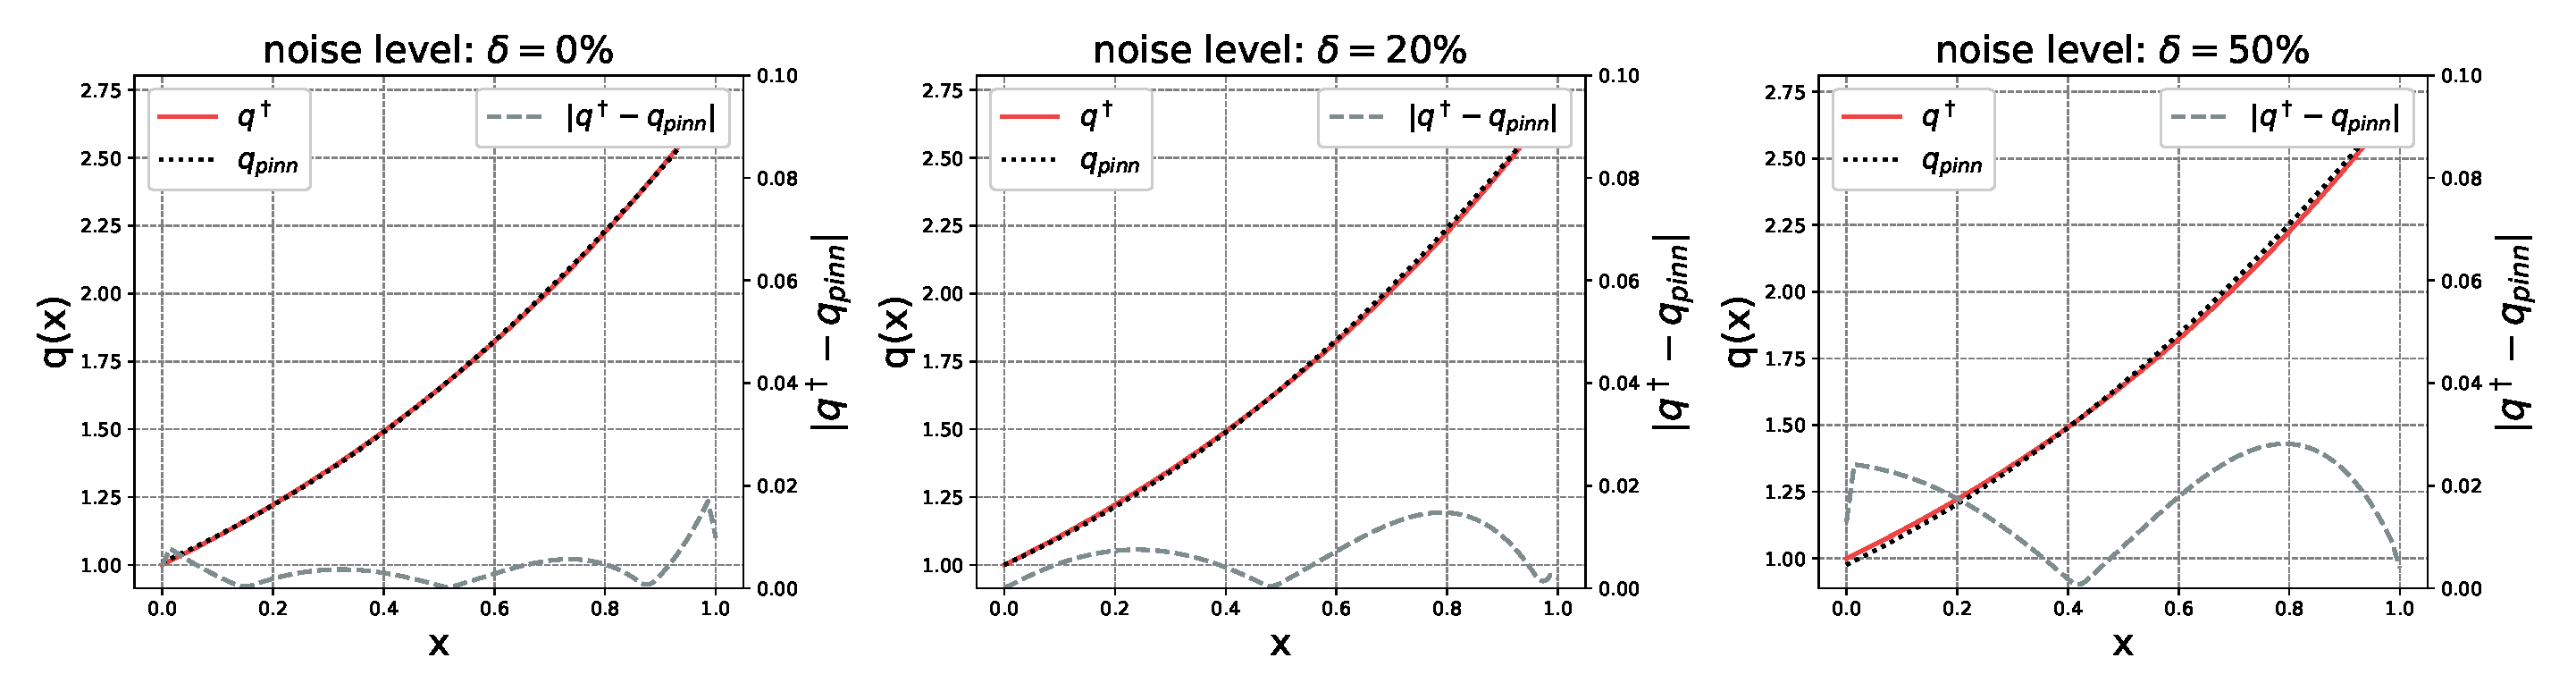
\includegraphics[width=\textwidth]{figures3/ex0_q.eps}
    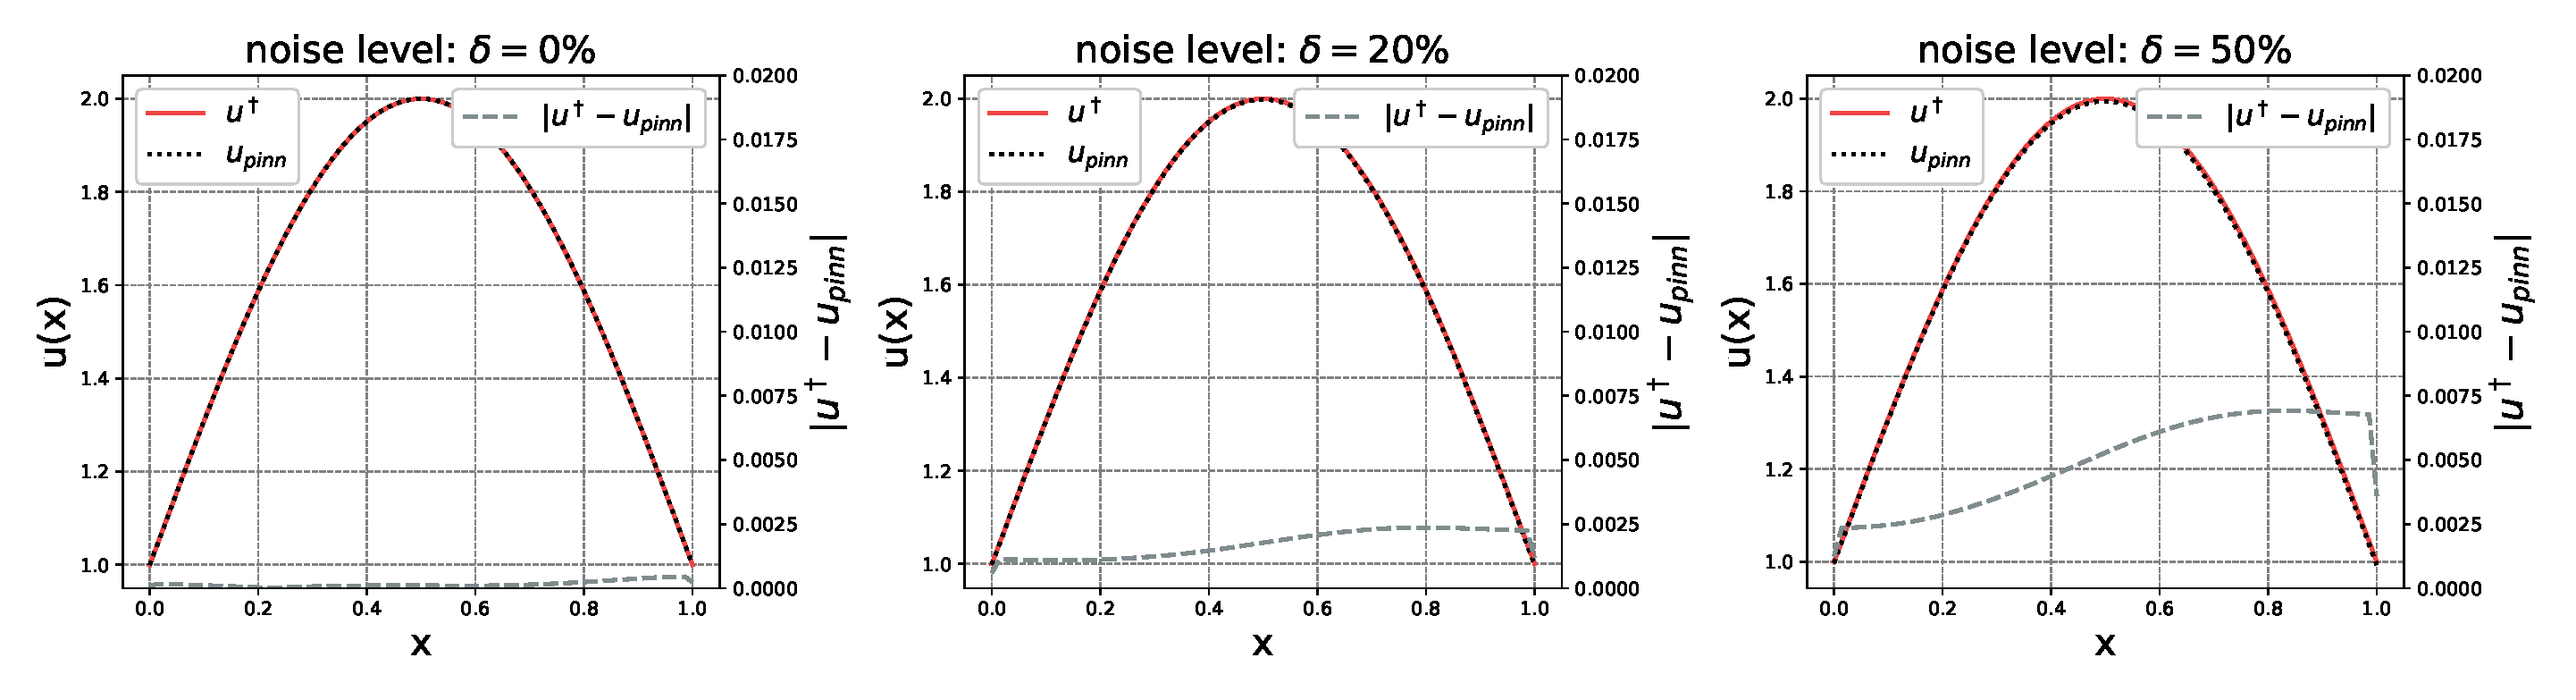
\includegraphics[width=\textwidth]{figures3/ex0_u.eps}
    \caption{例 \ref{example:1d} 的精确解、Tikhonov-PINN 解和绝对误差。第一行对应源项 $q$，第二行对应解 $u$。从左到右，结果是在不同的噪声水平下获得的。}
    \label{fig:ex0_q_u}
\end{figure}

在本小节中，我们使用一个一维例子来验证 Tikhonov-PINNs 的收敛率，并研究超参数对重构误差的影响。
\begin{example}\label{example:1d}
令 $\Omega=(0,1)$ 且 $\alpha\equiv 1$，定义精确势函数为 $q^{\dagger}(x)=\exp(x)$，对应的解为 $u^{\dagger}(x) = 1+\sin(\pi x)$。源项 $f$ 和边界条件 $g$ 由模型方程 Eq.\eqref{eq:pde:potential} 确定。
\end{example}

$q$ 和 $u$ 的精确解与 Tikhonov-PINNs 解如图 \ref{fig:ex0_q_u} 所示。在本例中，我们设置 $\lambda=10^{-7}$，采样 50,000 个内部点，并将边界点设为 \{0, 1\}。优化使用 Adam 优化器进行，学习率为 $10^{-4}$，迭代次数为 10,000 次。我们采用一个具有 $tanh$ 激活函数且宽度为 64 的两层神经网络来逼近 $q$ 和 $u$，并在架构中每两个相邻隐藏层之间应用残差连接。除非另有说明，本小节中的所有一维算例均使用与本例相同的默认参数设置。

\subsubsection{收敛率}
在定理 \ref{thm:ConvergenceRate} 中，我们建立了 $q$ 和 $u$ 关于噪声水平 $\delta$ 的收敛率。为了验证这一结果，我们计算了不同噪声水平下 $q$ 和 $u$ 的相对误差，结果如图 \ref{fig:ex0:noise} 所示。

\begin{figure}[htbp]
    \centering
    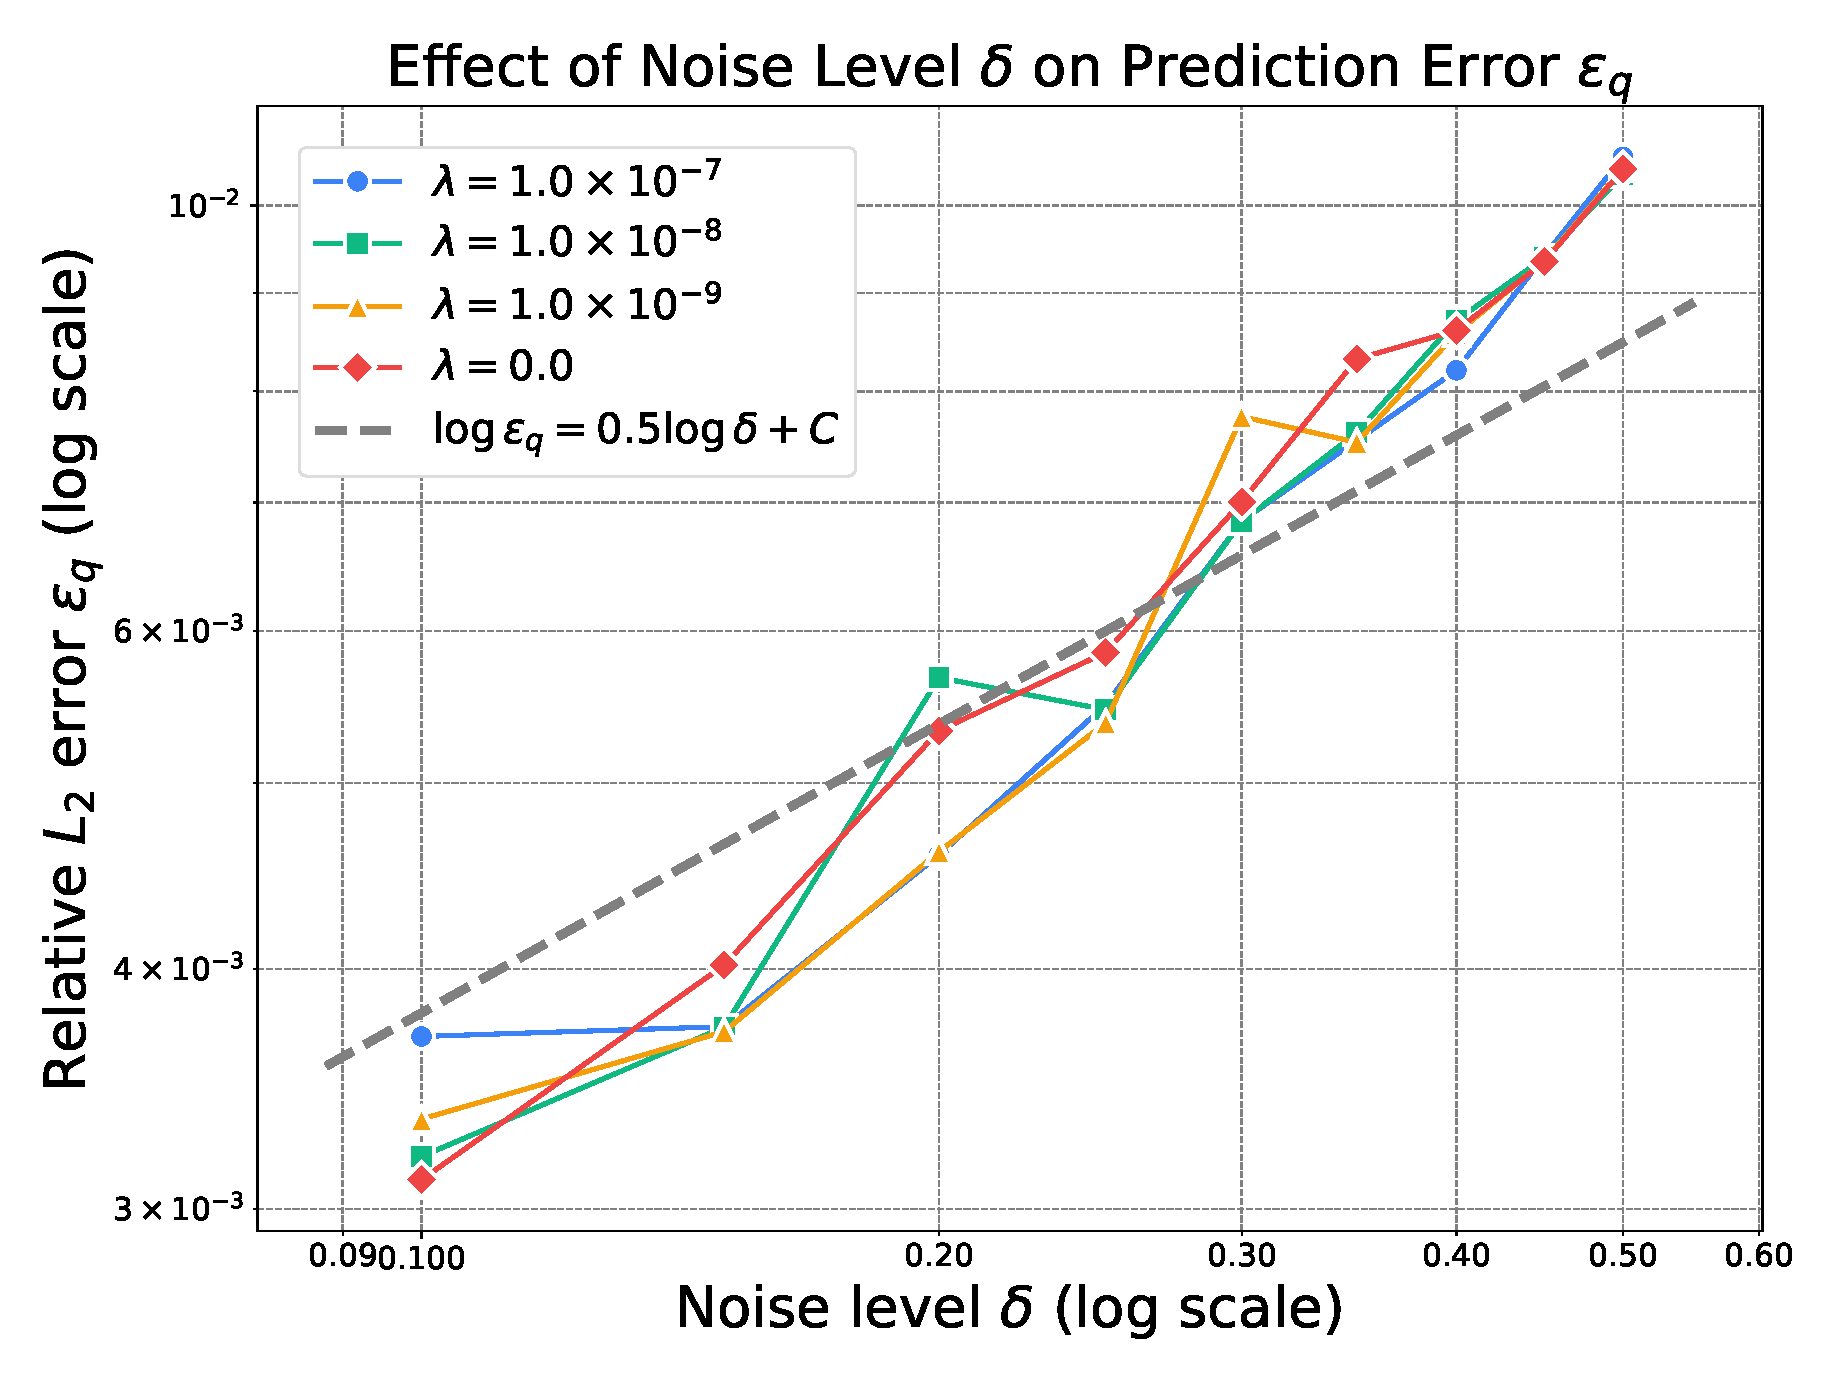
\includegraphics[width=0.49\textwidth]{figures3/ex0_noise_q.eps}
    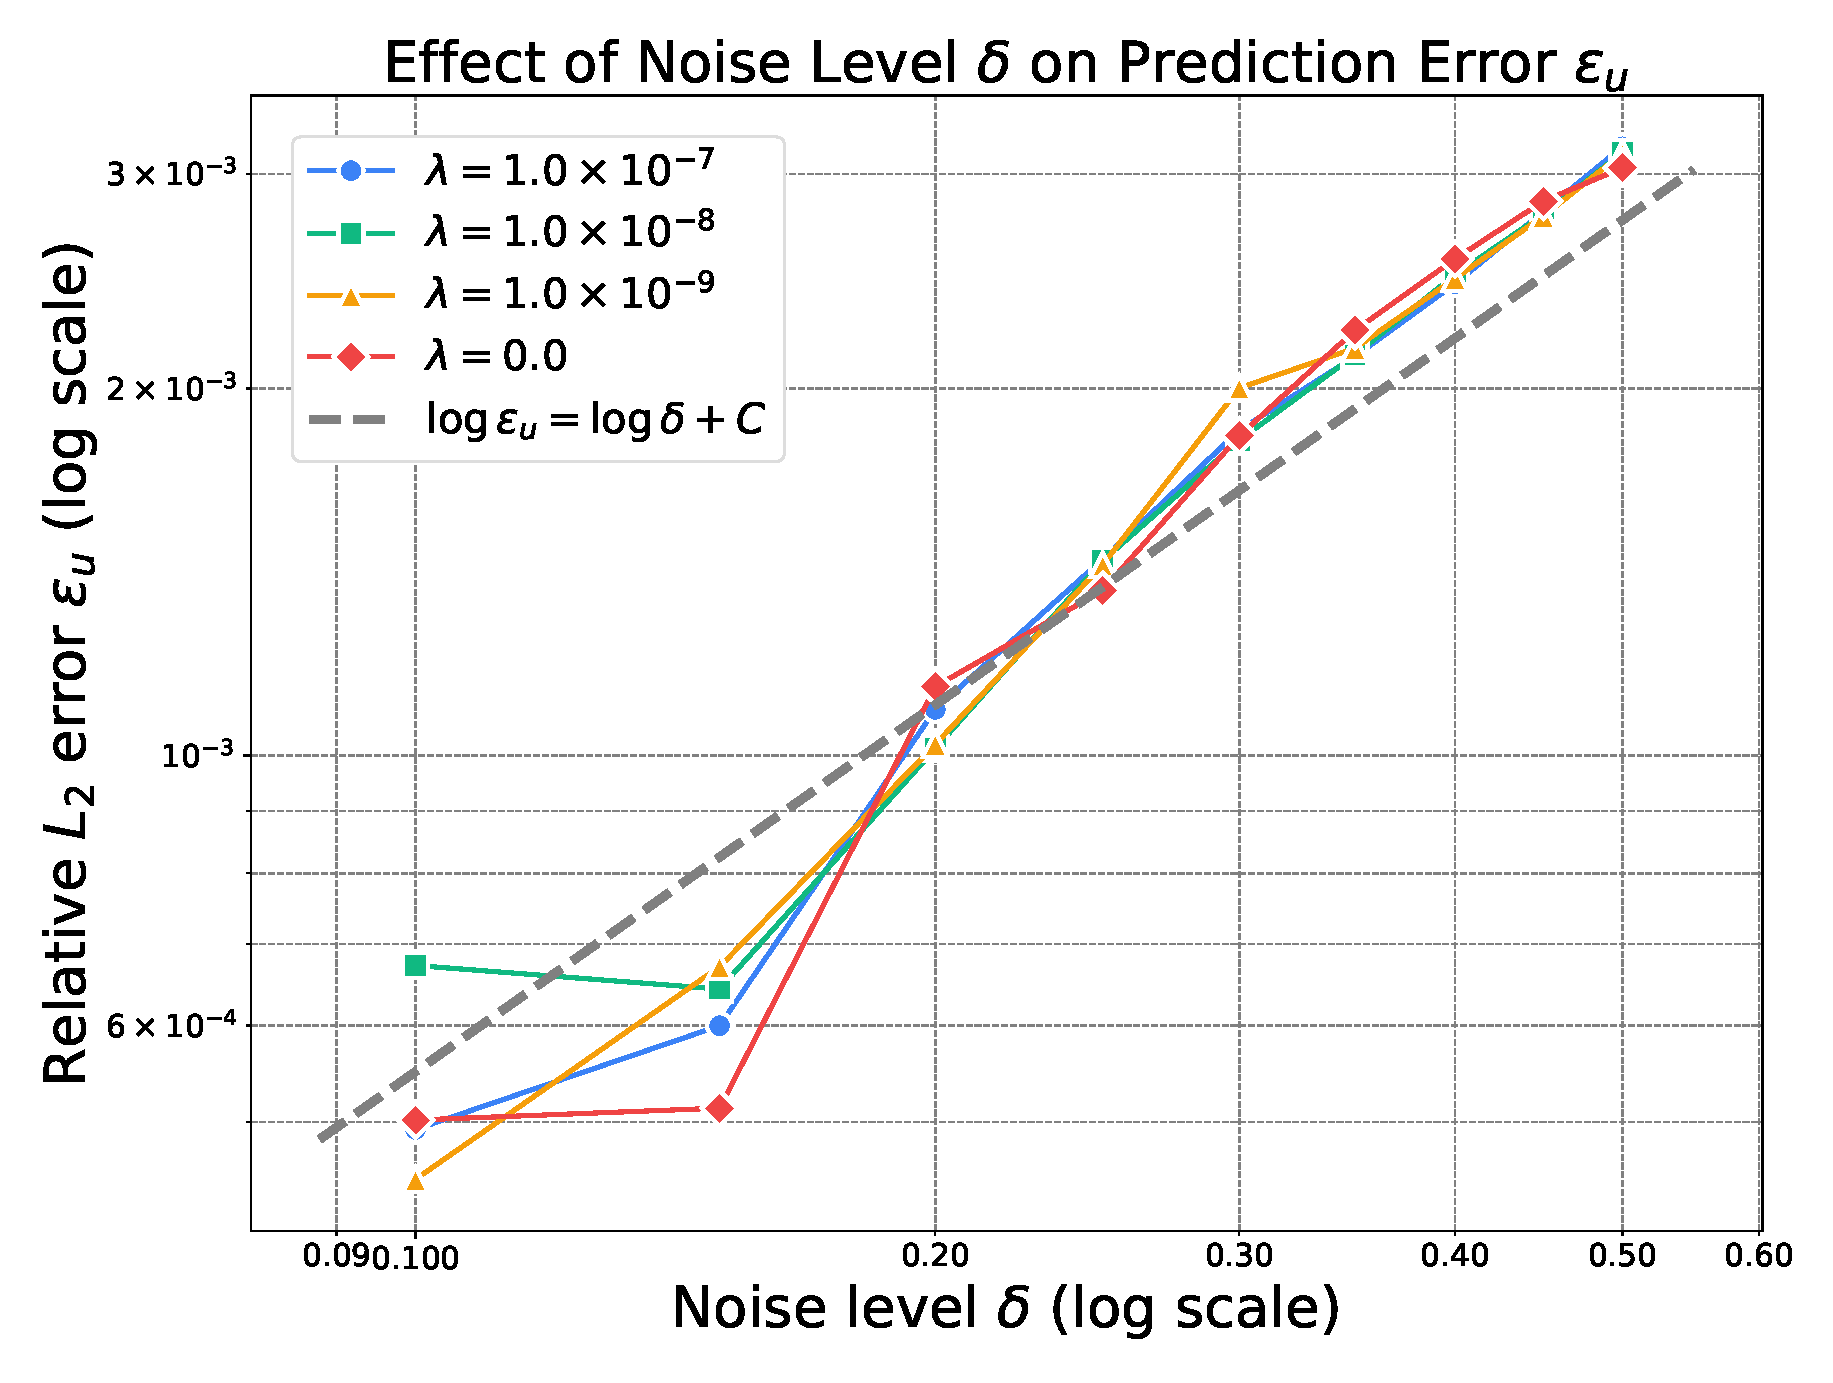
\includegraphics[width=0.49\textwidth]{figures3/ex0_noise_u.eps}
    \caption{不同正则化参数下噪声水平对解误差的影响。左图显示了 $q$ 的结果，其中 $\lambda=$$10^{-7}$, $10^{-8}$, $10^{-9}$ 和 0 对应的对数回归曲线的斜率分别为 0.708、0.748、0.760 和 0.743，平均斜率为 0.744。右图显示了 $u$ 的结果，其中对应的斜率分别为 1.22、1.08、1.25 和 1.26，平均斜率为 1.21。}
    \label{fig:ex0:noise}
\end{figure}

由于目标势函数具有正下界，该算例满足 $\beta = 0$ 的正性条件。根据定理~\ref{thm:ConvergenceRate} 和注 \ref{compare_Gar}，$q$ 和 $u$ 的收敛率可以任意接近 $O(\delta^{0.5})$ 和 $O(\delta)$。这一点在图 \ref{fig:ex0:noise} 中得到了检验，其中 $u$ 和 $q$ 的数值收敛率与理论收敛率非常一致。平均而言，在不同的 $\lambda$ 值下，我们观察到 $u$ 的经验收敛率为 $O(\delta^{1.21})$，$q$ 的经验收敛率为 $O(\delta^{0.74})$，这实际上快于理论收敛率，表明我们的理论界可能不是最优的。

\subsubsection{正则化的影响}
在本小节中，我们要研究不同正则化在求解算例 \ref{example:1d} 时的影响。如表 \ref{tab:regularization} 所示，当训练样本量相对较小（表 1 中的第一个子表）时，与 $L^2$ 正则化或原始 PINNs 相比，$H^2$ 正则化显著降低了 $q$ 的相对误差，尤其是当正则化系数 $\lambda$ 相对较大时。第二个子表表明，随着更多训练样本的可用，这种改进变得不那么明显。这是符合预期的，因为适当的正则化和增加数据量都有助于防止过拟合并提高精度。尽管如此，在两种情况下，当 $\lambda$ 选择得当时，$H^2$ 正则化都能产生最小的重构误差。这些结果凸显了 $H^2$ 正则化在求解此类反势问题时的有效性和优越性。

\begin{table}[hbtp]
\centering
\footnotesize
\caption{算例 \ref{example:1d} 中不同正则化下 $\hat{q}$ 的相对 $L^{2}$ 误差。}
\begin{tabular}{lrrrrr}
\hline
\multirow{2}[0]{*}{$\text{err}(q_{\text{pinn}})$} & \multicolumn{5}{c}{正则化参数 $\lambda$} \\
\cline{2-6}
& \multicolumn{1}{l}{$1.0\times 10^{-3}$} & 
\multicolumn{1}{l}{$1.0\times 10^{-4}$} &
\multicolumn{1}{l}{$1.0\times 10^{-5}$} &
\multicolumn{1}{l}{$1.0\times 10^{-6}$} & 
\multicolumn{1}{l}{$1.0\times 10^{-7}$} \\
   \hline
$H^2$ 正则化 & $5.44\times 10^{-2}$ & $\textbf{5.26}\times \textbf{10}^{-2}$ & $8.27\times 10^{-2}$ & $8.99\times 10^{-2}$ & $9.07\times 10^{-2}$ \\
$L^2$ 正则化 & $9.35\times 10^{-2}$ & $9.11\times 10^{-2}$ & $9.08\times 10^{-2}$ & $9.08\times 10^{-2}$ & $9.08\times 10^{-2}$ \\
无正则化 & $9.08\times 10^{-2}$ & $9.08\times 10^{-2}$ & $9.08\times 10^{-2}$ & $9.08\times 10^{-2}$ & $9.08\times 10^{-2}$  \\
\hline
&       &       &       &       & \\
\hline
\multirow{2}[0]{*}{$\text{err}(q_{\text{pinn}})$} & \multicolumn{5}{c}{正则化参数 $\lambda$} \\
\cline{2-6}
& \multicolumn{1}{l}{$1.0\times 10^{-3}$} & 
\multicolumn{1}{l}{$1.0\times 10^{-4}$} &
\multicolumn{1}{l}{$1.0\times 10^{-5}$} &
\multicolumn{1}{l}{$1.0\times 10^{-6}$} & 
\multicolumn{1}{l}{$1.0\times 10^{-7}$} \\
\hline
$H^2$ 正则化 & $8.96\times 10^{-2}$ & $3.14\times 10^{-2}$ & $\textbf{2.94}\times \textbf{10}^{-2}$ & $3.03\times 10^{-2}$ & $3.04\times 10^{-2}$  \\
$L^2$ 正则化 & $3.80\times 10^{-2}$ & $3.10\times 10^{-2}$ & $3.05\times 10^{-2}$ & $3.04\times 10^{-2}$ & $3.04\times 10^{-2}$ \\
无正则化 & $3.04\times 10^{-1}$ & $3.04\times 10^{-2}$ & $3.04\times 10^{-2}$ & $3.04\times 10^{-2}$ & $3.04\times 10^{-2}$ \\
\hline

\end{tabular}
\label{tab:regularization}
\end{table}

\subsubsection{其他超参数的影响}

\begin{figure}[htbp]
    \centering
    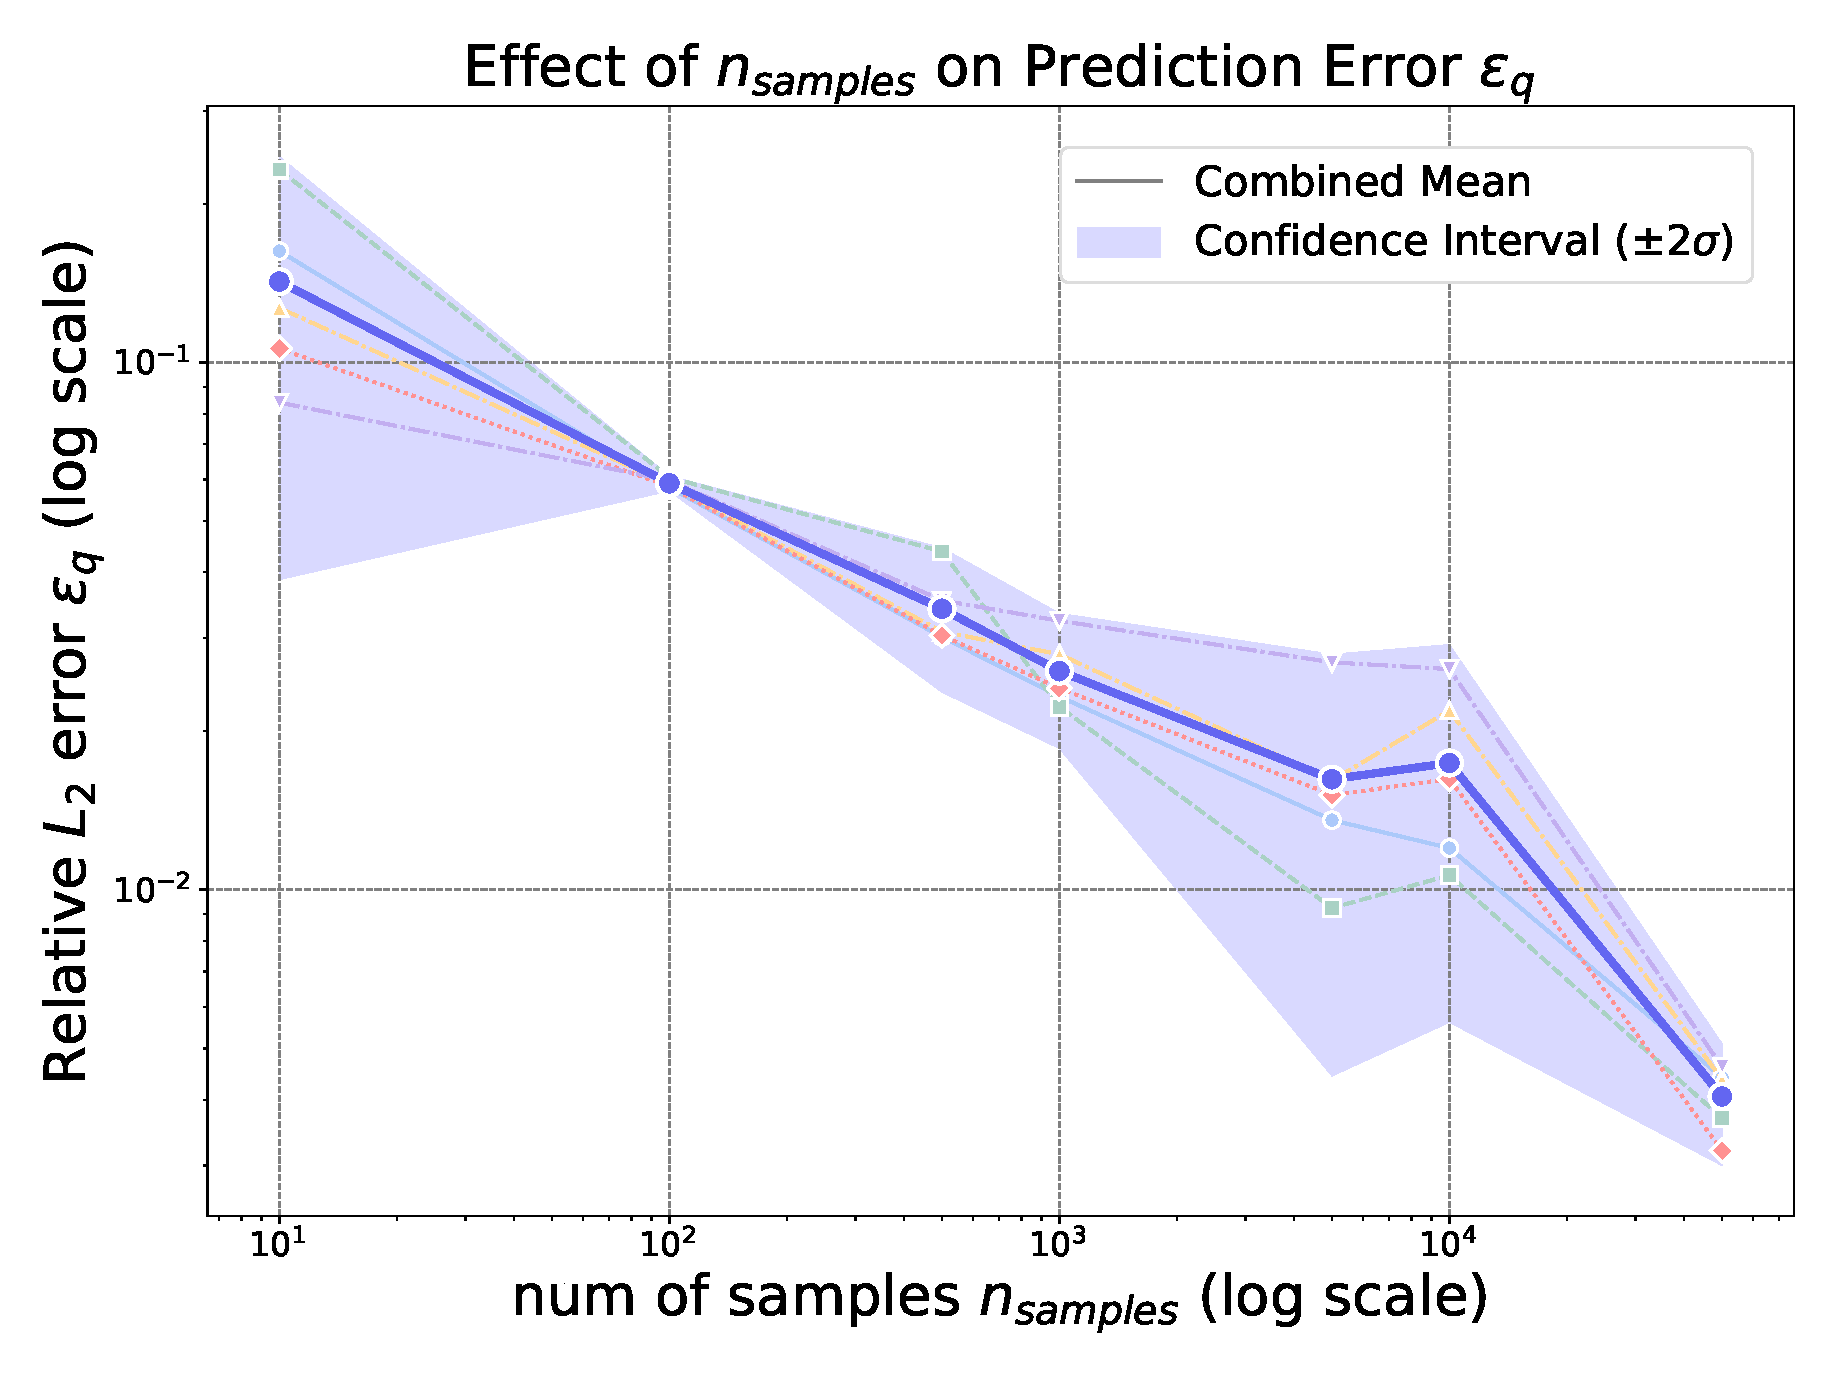
\includegraphics[width=0.48\textwidth]{figures3/ex0_nsample.eps}
    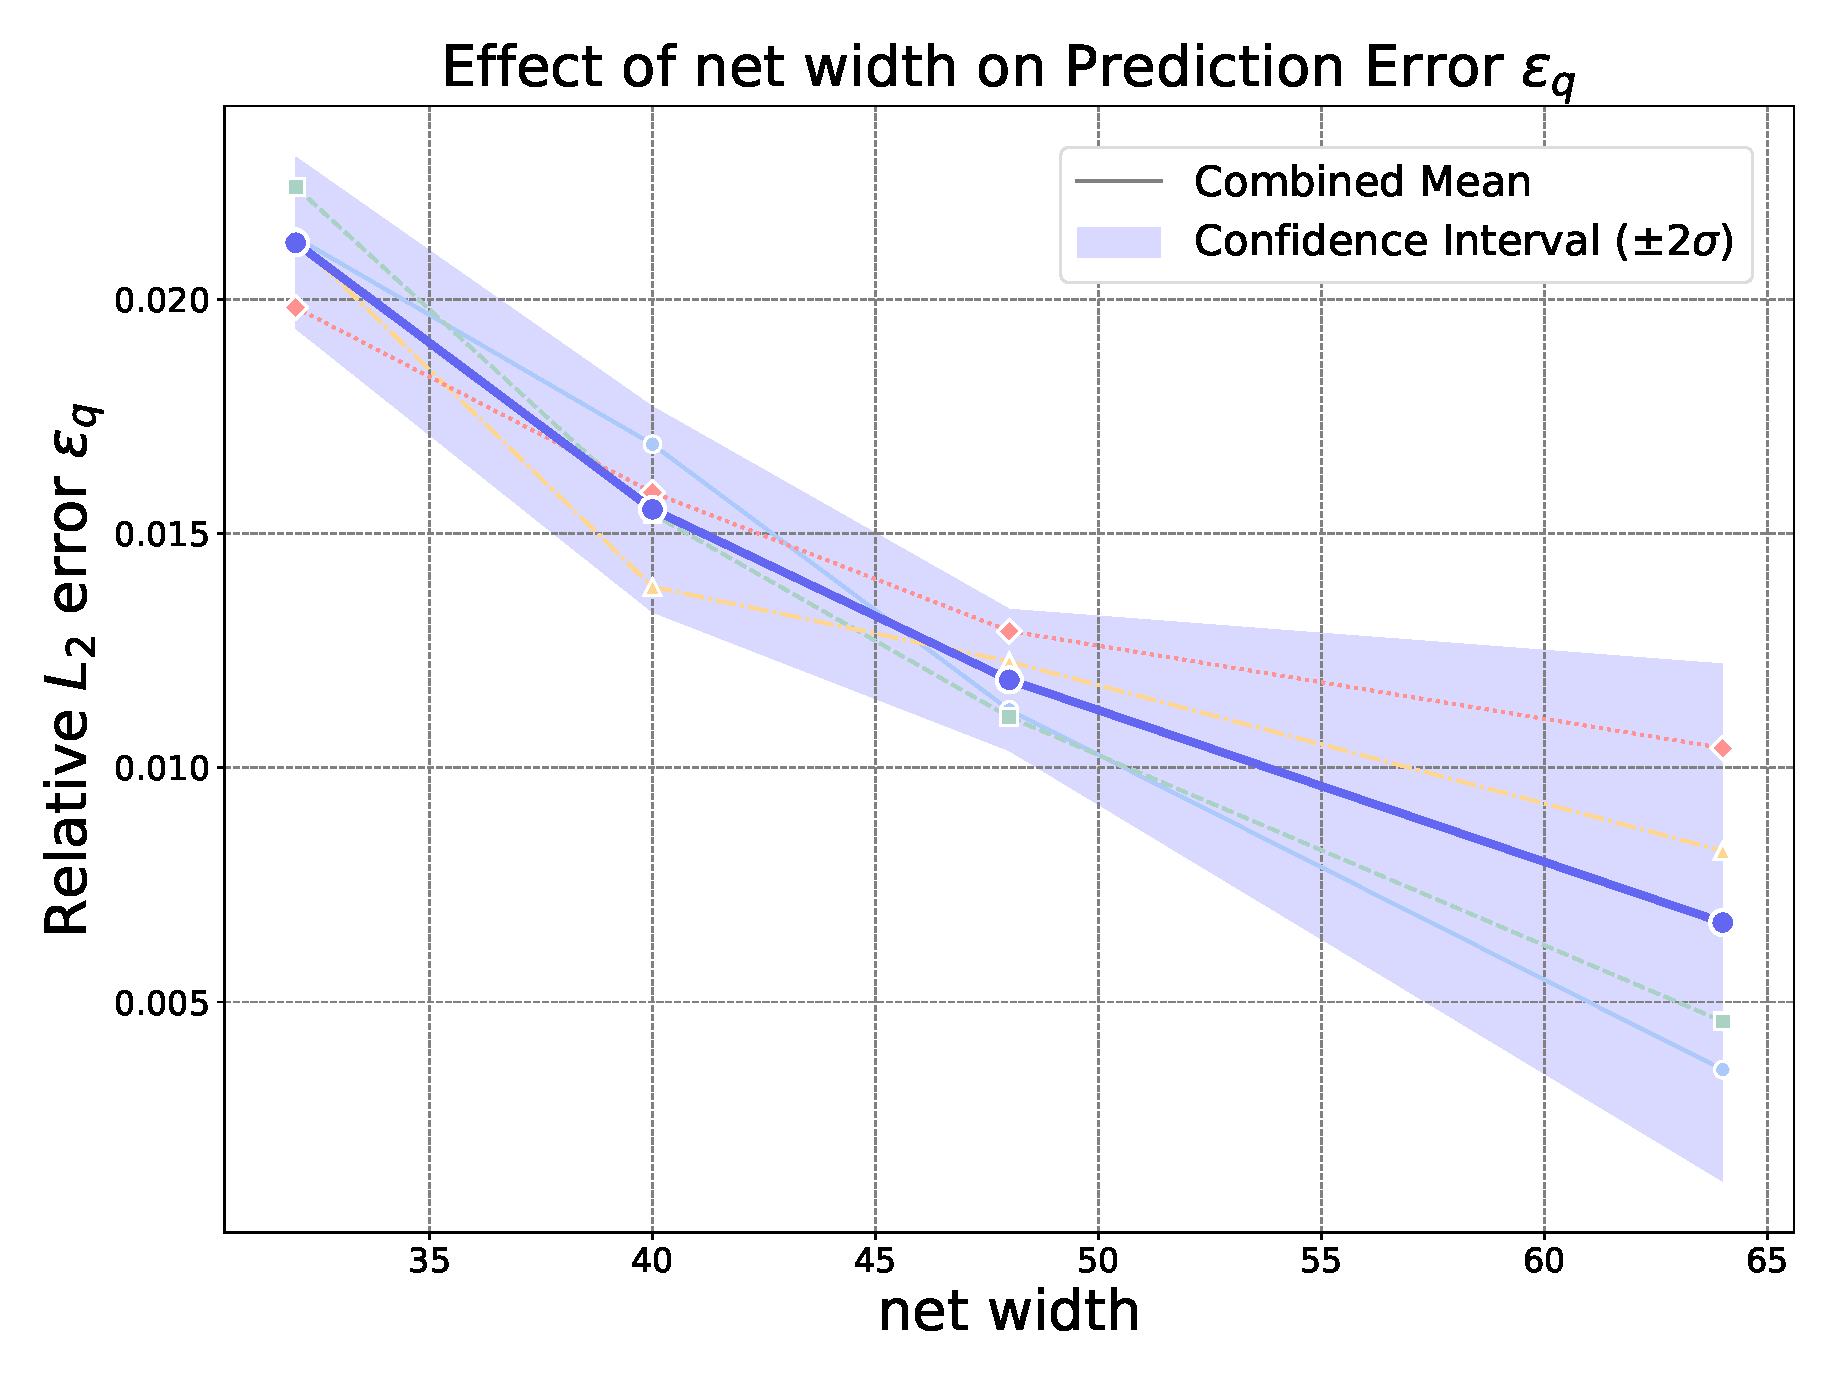
\includegraphics[width=0.48\textwidth]{figures3/ex0_width.eps}
    \caption{样本大小和网络宽度对算法精度的影响。我们进行了多次运行，并展示了相应的置信区间。特别地，由于网络深度是固定的，非零参数的数量 $R_{\calQ}$ 与网络宽度近似成正比。}
    \label{fig:ex0:width}
\end{figure}

我们研究了神经网络复杂度和样本复杂度对模型性能的影响。根据定理 \ref{thm:ConvergenceRate} 和假设 \ref{allcondition}，要实现更低的重构误差，需要增加样本大小和网络规模。我们通过以下实验验证了这种单调关系。在图~\ref{fig:ex0:width} 左侧，我们固定网络架构并改变样本大小以考察其影响。在图~\ref{fig:ex0:width} 右侧，我们保持两层的网络深度，同时调整网络宽度，从而按比例缩放神经元总数 $R_\mathbf{\calQ}$。对每个设置都进行了多次运行，图中显示的结果表明，误差随着样本大小和参数数量的增加而减小。

\subsubsection{二维问题}
接下来我们展示一个二维光滑算例，其中待反演的 $q^{\dagger}$ 和 $u^{\dagger}$ 均呈现正弦函数形式。

\begin{example}\label{example:onemode}
令 $\Omega=(0,1)^{2}$ 且 $\alpha\equiv 1$。我们考虑对以下势函数的识别
\begin{equation*}
q^{\dagger}(x_{1},x_{2})=1+0.5\times\sin(\pi x_{1})\sin(\pi x_{2}),
\end{equation*}
且精确解 $u^{\dagger}$ 为：
\[
u^{\dagger}(x_{1},x_{2})=1+\sin(\pi x_{1})\sin(\pi x_{2}).
\]
\end{example}

在本实验中，神经网络包含两个宽度为 64 的隐藏层。我们在内部和边界上共采样 100,000 个点，并使用学习率为 $10^{-4}$ 的 Adam 优化器训练模型 50,000 次迭代。

我们还使用有限元方法 (FEM) 求解了相同的问题。在 FEM 实现中，采用了一阶拉格朗日单元，并利用 L-BFGS 算法对解进行了 50 次迭代优化。为了确保比较的公平性，区域 $[0,1]^2$ 被离散化为 $320\times 320=102,400$ 个网格点，这与 Tikhonov-PINNs 中使用的总样本数（$100,000$ 个样本）相当。

\begin{figure}[htbp]
    \centering
    % 第一个子图：Tikhonov-PINNs 方法（假设文件名暗示这是神经网络方法）
    \begin{subfigure}[b]{\textwidth}
        \centering
        % 插入图片
        \includegraphics[width=\textwidth]{figures3/one_peak_nn.eps}
        % 简短的子标题
        \caption{Tikhonov-PINNs 方法结果}
        \label{fig:one_peak_nn}
    \end{subfigure}
    \hfill % 填充中间空白，让图片分别对齐左右
    % 第二个子图：有限元方法 (FEM)
    \begin{subfigure}[b]{\textwidth}
        \centering
        % 插入图片
        \includegraphics[width=\textwidth]{figures3/one_peak_fem.eps}
        % 简短的子标题
        \caption{有限元方法 (FEM) 结果}
        \label{fig:one_peak_fem}
    \end{subfigure}
    
    % 总标题：包含详细描述
    \caption{两种方法重构结果的比较：(a) Tikhonov-PINNs 和 (b) 有限元方法 (FEM)。
    左侧小图展示了例 \ref{example:onemode} 中势函数 $q^{\dagger}$（上）和解 $u^{\dagger}$（下）的真值；
    右侧小图展示了在不同噪声水平 $\delta$ 下，使用最优正则化参数 $\lambda$ 重构的势 $\hat{q}$ 和解 $\hat{u}$。}
    \label{fig:example:one_peak}
\end{figure}


数值结果如图~\ref{fig:example:one_peak} 所示。这里，基于各种实验，$\lambda$ 被选为最优正则化参数。为了进一步阐明噪声 $\delta$ 的影响，我们在表~\ref{tab:onemode} 中提供了不同正则化参数 $\lambda$ 下相对误差的详细比较。显然，在低噪声水平下，FEM 和 Tikhonov-PINNs 方法均能有效地重构 $q$ 和 $u$。此外，随着噪声水平的增加，$q$ 的误差逐渐增大，这与我们的理论发现相符。在大多数情况下，FEM 优于 Tikhonov-PINNs 方法，当 $\lambda$ 选择得当时，产生的相对 $L^2$ 误差更低。这突显了 FEM 在处理此类光滑问题时的优越性，特别是在低维情况下。然而，正如第~\ref{sec:semi_converge} 节所讨论的，FEM 中的半收敛现象需要仔细的早停策略。此外，对于非光滑和高维问题，Tikhonov-PINNs 表现出优于标准 FEM 的性能。我们将在后续章节中对此进行讨论。

聚焦于 Tikhonov-PINNs 的结果，很明显，较高的噪声水平需要较大的正则化参数 $\lambda$，以在重构解中获得最佳的误差控制。噪声强度与正则化参数之间的这种单调关系与定理~\ref{thm:ConvergenceRate} 中的分析一致。

\begin{table}[htbp]
   \centering
   \footnotesize
   \caption{例 \ref{example:onemode} 中重构势 $\hat{q}$ 和解 $\hat{u}$ 的相对 $L^{2}$ 误差。}
   \begin{tabular}{lllllll}
   \hline
   \multirow{2}[0]{*}{$\delta  = 1\%$} & \multicolumn{6}{c}{正则化参数 $\lambda$} \\
   \cline{2-7}
   & $1.0\times 10^{-5}$ & $1.0\times 10^{-6}$ & $1.0\times 10^{-7}$ & $1.0\times 10^{-8}$ & $1.0\times 10^{-9}$ & \multicolumn{1}{r}{0} \\
   \hline
   $\text{err}(u_{\text{pinn}})$ & $3.14\times 10^{-3}$ & $1.49\times 10^{-3}$ & $7.67\times 10^{-4}$ & $5.99\times 10^{-4}$ & $5.81\times 10^{-4}$ & $5.72\times 10^{-4}$ \\
   $\text{err}(u_{\text{fem}})$ & $1.93\times 10^{-4}$ & $1.84\times 10^{-4}$ & $1.19\times 10^{-4}$ & $1.44\times 10^{-4}$ & $1.68\times 10^{-4}$ & $1.03\times 10^{-4}$ \\
   $\text{err}(q_{\text{pinn}})$ & $1.46\times 10^{-1}$ & $5.39\times 10^{-2}$ & $3.39\times 10^{-2}$ & $3.27\times 10^{-2}$ & $3.27\times 10^{-2}$ & $3.27\times 10^{-2}$ \\
   $\text{err}(q_{\text{fem}})$ & $1.44\times 10^{-2}$ & \textbf{1.23$\times $10$^{-2}$} & $6.26\times 10^{-3}$ & $1.27\times 10^{-2}$ & $1.68\times 10^{-2}$ & $1.95\times 10^{-2}$ \\
   \hline
   &       &       &       &       &       &  \\
   \hline
   \multirow{2}[0]{*}{$\delta = 10\%$} & \multicolumn{6}{c}{正则化参数 $\lambda$} \\
   \cline{2-7}
   & $1.0\times 10^{-5}$ & $1.0\times 10^{-6}$ & $1.0\times 10^{-7}$ & $1.0\times 10^{-8}$ & $1.0\times 10^{-9}$ & \multicolumn{1}{r}{0} \\
   \hline
   $\text{err}(u_{\text{pinn}})$ & $3.08\times 10^{-3}$ & $1.97\times 10^{-3}$ & $1.48\times 10^{-3}$ & $1.41\times 10^{-3}$ & $1.40\times 10^{-3}$ & $1.40\times 10^{-3}$ \\
   $\text{err}(u_{\text{fem}})$ & $1.09\times 10^{-3}$ & $6.30\times 10^{-4}$ & $1.71\times 10^{-3}$ & $2.51\times 10^{-3}$ & $2.71\times 10^{-3}$ & $3.43\times 10^{-3}$\\
   $\text{err}(q_{\text{pinn}})$ & $1.50\times 10^{-1}$ & $6.18\times 10^{-2}$ & $4.33\times 10^{-2}$ & $4.13\times 10^{-2}$ & $4.11\times 10^{-2}$ & $4.11\times 10^{-2}$ \\
   $\text{err}(q_{\text{fem}})$ & \textbf{1.72$\times $10$^{-2}$} & $2.84\times 10^{-2}$ & $8.56\times 10^{-2}$ & $3.23\times 10^{-1}$ & $3.80\times 10^{-1}$ & $5.40\times 10^{-1}$\\
   \hline
   &       &       &       &       &       &  \\
   \hline
   \multirow{2}[0]{*}{$\delta = 20\%$} & \multicolumn{6}{c}{正则化参数 $\lambda$} \\
   \cline{2-7}
   & $1.0\times 10^{-5}$ & $1.0\times 10^{-6}$ & $1.0\times 10^{-7}$ & $1.0\times 10^{-8}$ & $1.0\times 10^{-9}$ & \multicolumn{1}{r}{0} \\
   \hline
   $\text{err}(u_{\text{pinn}})$ & $3.38\times 10^{-3}$ & $2.47\times 10^{-3}$ & $2.19\times 10^{-3}$ & $2.17\times 10^{-3}$ & $2.17\times 10^{-3}$ & $2.17\times 10^{-3}$ \\
   $\text{err}(u_{\text{fem}})$ & $8.88\times 10^{-4}$ & $2.16\times 10^{-3}$ & $4.76\times 10^{-3}$ & $4.30\times 10^{-3}$ & $3.44\times 10^{-3}$ & $4.98\times 10^{-3}$ \\
   $\text{err}(q_{\text{pinn}})$ & $1.54\times 10^{-1}$ & $7.29\times 10^{-2}$ & $6.34\times 10^{-2}$ & $6.44\times 10^{-2}$ & $6.46\times 10^{-2}$ & $6.46\times 10^{-2}$ \\
   $\text{err}(q_{\text{fem}})$ & \textbf{1.89$\times $10$^{-2}$} & $8.56\times 10^{-2}$ & $2.64\times 10^{-1}$ & $3.85\times 10^{-1}$ & $4.35\times 10^{-1}$ & $4.98\times 10^{-1}$\\
   \hline
   &       &       &       &       &       &  \\
   \hline
   \multirow{2}[0]{*}{$\delta = 50\%$} & \multicolumn{6}{c}{正则化参数 $\lambda$} \\
   \cline{2-7}
   & $1.0\times 10^{-5}$ & $1.0\times 10^{-6}$ & $1.0\times 10^{-7}$ & $1.0\times 10^{-8}$ & $1.0\times 10^{-9}$ & \multicolumn{1}{r}{0} \\
   \hline
   $\text{err}(u_{\text{pinn}})$ & $4.14\times 10^{-3}$ & $5.22\times 10^{-3}$ & $5.20\times 10^{-3}$ & $5.22\times 10^{-3}$ & $5.22\times 10^{-3}$ & $5.22\times 10^{-3}$ \\
   $\text{err}(u_{\text{fem}})$ & $4.90\times 10^{-3}$ & $7.22\times 10^{-3}$ & $8.26\times 10^{-3}$ & $1.01\times 10^{-2}$ & $1.40\times 10^{-2}$ & $9.21\times 10^{-3}$ \\
   $\text{err}(q_{\text{pinn}})$ & $1.65\times 10^{-1}$ & $1.03\times 10^{-1}$ & $1.05\times 10^{-1}$ & $1.06\times 10^{-1}$ & $1.06\times 10^{-1}$ & $1.06\times 10^{-1}$ \\
   $\text{err}(q_{\text{fem}})$ & \textbf{5.64$\times $10$^{-2}$} & $2.32\times 10^{-1}$ & $5.85\times 10^{-1}$ & $0.85\times 10^{-1}$ & $1.10$ & $0.81\times 10^{-1}$\\
   \hline
   \end{tabular}
   \label{tab:onemode}%
\end{table}%

% \subsection{非光滑势问题}
% 为了进一步探索我们算法的局限性并评估神经网络对非光滑势的逼近能力，我们将我们的方法应用于几个非光滑算例，在这些算例中，诸如标准有限元方法 (FEM) 等传统方法的效果可能较差。参数设置保持与算例~\ref{example:onemode} 中相同。此外，我们将 Tikhonov-PINNs 方法的性能与经典有限元方法进行了比较。本节的 FEM 设置与算例 5.2 中的设置相同。

% \subsubsection{连续问题}
% 接下来，我们考虑如下定义的非光滑势函数的识别问题。

% \begin{example}\label{example:nonsmooth}
% % Table generated by Excel2LaTeX from sheet '5'
% 令 $\Omega=(0,1)^{2}$ 且 $\alpha\equiv 1$。定义精确势函数 $q^{\dagger}$ 为：
% \begin{align*}
% \zeta(x_{1},x_{2})&=\exp\{-25\times(x_{1}-0.6)^{2}-25\times(x_{2}-0.4)^{2}\}, \\
% q^{\dagger}(x_{1},x_{2})&=0.75+\min\{0.75,\max\{0.25,2\zeta(x_{1},x_{2})\}\},
% \end{align*}
% 精确解 $u^{\dagger}$ 为 $u^{\dagger}(x_{1},x_{2})=1+\sin(\pi x_{1})\sin(\pi x_{2})$。
% \end{example}
% 表 \ref{tab:nonsmooth} 展示了在不同 $\lambda$ 和 $\delta$ 下 $u$ 和 $q$ 的相对误差，并用粗体高亮了每种噪声水平下的最佳结果。正如我们所见，Tikhonov-PINNs 在所有配置下始终实现了约为 $\calO(10^{-2})$ 的 $q$ 相对误差，比有限元方法高出一个数量级。


% \begin{table}[htbp]
%    \centering
%    \footnotesize
%    \caption{Example \ref{example:nonsmooth} 中恢复的势 $\hat{q}$ 和解 $\hat{u}$ 的相对 $L^{2}$ 误差。}
%    \begin{tabular}{lllllll}
%    \hline
%    \multirow{2}[0]{*}{$\delta  = 1\%$} & \multicolumn{6}{c}{正则化参数 $\lambda$} \\
%    \cline{2-7}
%    & $1.0\times 10^{-5}$ & $1.0\times 10^{-6}$ & $1.0\times 10^{-7}$ & $1.0\times 10^{-8}$ & $1.0\times 10^{-9}$ & \multicolumn{1}{r}{0} \\
%    \hline
%    $\text{err}(u_{\text{pinn}})$ & $3.14\times 10^{-3}$ & $2.01\times 10^{-3}$ & $6.03\times 10^{-4}$ & $5.71\times 10^{-4}$ & $4.94\times 10^{-4}$ & $4.03\times 10^{-4}$ \\
%    $\text{err}(u_{\text{fem}})$& $2.60\times 10^{-3}$& $1.14\times 10^{-3}$& $7.09\times 10^{-4}$& $6.96\times 10^{-4}$ & $5.33\times 10^{-4}$ &$6.41\times 10^{-4}$\\
%    $\text{err}(q_{\text{pinn}})$ & $1.46\times 10^{-1}$& $9.63\times 10^{-2}$ & $1.82\times 10^{-2}$ & $1.60\times 10^{-2}$ & \textbf{1.57$\times$ 10$^{-2}$} & \textbf{1.57$\times$ 10$^{-2}$}   \\
%    $\text{err}(q_{\text{fem}})$& $1.28\times 10^{-1}$& $8.77\times 10^{-2}$& $7.39\times 10^{-2}$& $7.36\times 10^{-2}$ & $6.43\times 10^{-2}$ &$6.97\times 10^{-2}$\\
%    \hline
%    &       &       &       &       &       &  \\
%    \hline
%    \multirow{2}[0]{*}{$\delta = 10\%$} & \multicolumn{6}{c}{正则化参数 $\lambda$} \\
%    \cline{2-7}
%    & $1.0\times 10^{-5}$ & $1.0\times 10^{-6}$ & $1.0\times 10^{-7}$ & $1.0\times 10^{-8}$ & $1.0\times 10^{-9}$ & \multicolumn{1}{r}{0} \\
%    \hline
%    $\text{err}(u_{\text{pinn}})$ & $3.08\times 10^{-3}$ & $2.22\times 10^{-3}$ & $1.36\times 10^{-3}$ & $1.30\times 10^{-3}$ & $1.30\times 10^{-3}$ & $1.30\times 10^{-3}$ \\
%    $\text{err}(u_{\text{fem}})$& $2.82\times 10^{-3}$& $1.30\times 10^{-3}$& $1.44\times 10^{-3}$& $1.18\times 10^{-3}$ & $1.30\times 10^{-3}$&$2.36\times 10^{-3}$\\
%    $\text{err}(q_{\text{pinn}})$ & $1.50\times 10^{-1}$ & $1.03\times 10^{-1}$ & $1.78\times 10^{-2}$ & $1.60\times 10^{-2}$ & $1.71\times 10^{-2}$ & \textbf{1.58$\times$ 10$^{-2}$ }\\
%    $\text{err}(q_{\text{fem}})$& $1.29\times 10^{-1}$& $8.77\times 10^{-2}$& $7.95\times 10^{-2}$& $9.02\times 10^{-2}$ & $1.16\times 10^{-1}$&$1.90\times 10^{-1}$\\
%    \hline
%    &       &       &       &       &       &  \\
%    \hline
%    \multirow{2}[0]{*}{$\delta = 20\%$} & \multicolumn{6}{c}{正则化参数 $\lambda$} \\
%    \cline{2-7}
%    & $1.0\times 10^{-5}$ & $1.0\times 10^{-6}$ & $1.0\times 10^{-7}$ & $1.0\times 10^{-8}$ & $1.0\times 10^{-9}$ & \multicolumn{1}{r}{0} \\
%    \hline
%    $\text{err}(u_{\text{pinn}})$ & $3.38\times 10^{-3}$ & $2.30\times 10^{-3}$ & $1.44\times 10^{-3}$ & $1.35\times 10^{-3}$ & $1.36\times 10^{-3}$ & $1.36\times 10^{-3}$ \\
%    $\text{err}(u_{\text{fem}})$& $2.67\times 10^{-3}$& $2.17\times 10^{-3}$& $4.23\times 10^{-3}$&$ 3.75\times 10^{-3}$ & $2.50\times 10^{-3}$&$4.15\times 10^{-3}$\\
%    $\text{err}(q_{\text{pinn}})$ & $1.54\times 10^{-1}$ & $9.09\times 10^{-2}$ & $1.71\times 10^{-2}$ & $1.60\times 10^{-2}$ & \textbf{1.59$\times$ 10$^{-2}$} & \textbf{1.59$\times$ 10$^{-2}$} \\
%    $\text{err}(q_{\text{fem}})$& $1.27\times 10^{-1}$& $9.77\times 10^{-2}$& $2.21\times 10^{-1}$& $2.13\times 10^{-1}$ & $1.51\times 10^{-1}$&$3.79\times 10^{-1}$\\
%    \hline
%    &       &       &       &       &       &  \\
%    \hline
%    \multirow{2}[0]{*}{$\delta = 50\%$} & \multicolumn{6}{c}{正则化参数 $\lambda$} \\
%    \cline{2-7}
%    & $1.0\times 10^{-5}$ & $1.0\times 10^{-6}$ & $1.0\times 10^{-7}$ & $1.0\times 10^{-8}$ & $1.0\times 10^{-9}$ & \multicolumn{1}{r}{0} \\
%    \hline
%    $\text{err}(u_{\text{pinn}})$ & $4.14\times 10^{-3}$ & $4.43\times 10^{-3}$ & $4.07\times 10^{-3}$ & $3.43\times 10^{-3}$ & $4.01\times 10^{-3}$ & $4.04\times 10^{-3}$ \\
%    $\text{err}(u_{\text{fem}})$& $4.41\times 10^{-3}$& $7.14\times 10^{-3}$& $7.90\times 10^{-3}$& $7.64\times 10^{-3}$& $1.26\times 10^{-2}$&$8.40\times 10^{-3}$\\
%    $\text{err}(q_{\text{pinn}})$ & $1.65\times 10^{-1}$ & $1.22\times 10^{-1}$ & $6.30\times 10^{-2}$ & \textbf{3.16}$\times$ \textbf{10}$^{-2}$ & $4.99\times 10^{-2}$ & $5.14\times 10^{-1}$ \\
%    $\text{err}(q_{\text{fem}})$& $1.45\times 10^{-1}$& $2.14\times 10^{-1}$& $4.64\times 10^{-1}$& $4.09\times 10^{-1}$& $9.07\times 10^{-1}$&$5.90\times 10^{-1}$\\
%    \hline
%    \end{tabular}%
%    \label{tab:nonsmooth}%
% \end{table}%

% \begin{figure}[htbp]
% \centering
% \setlength{\abovecaptionskip}{10pt}
% 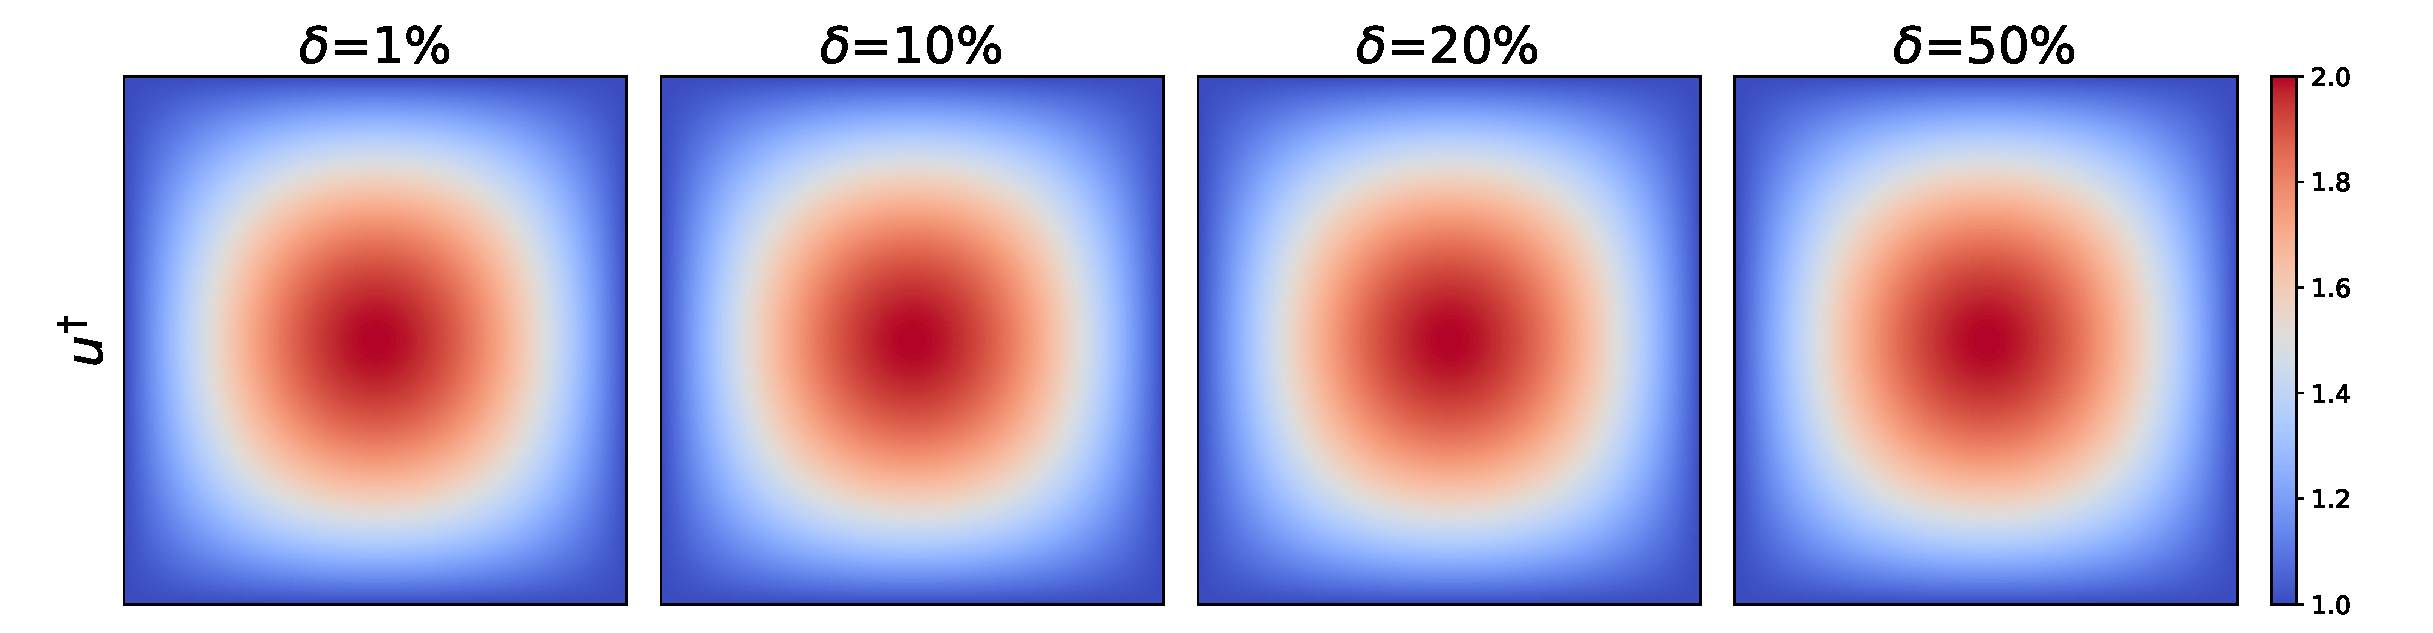
\includegraphics[width=\textwidth]{figures3/non_smooth_udag.eps}\par
% 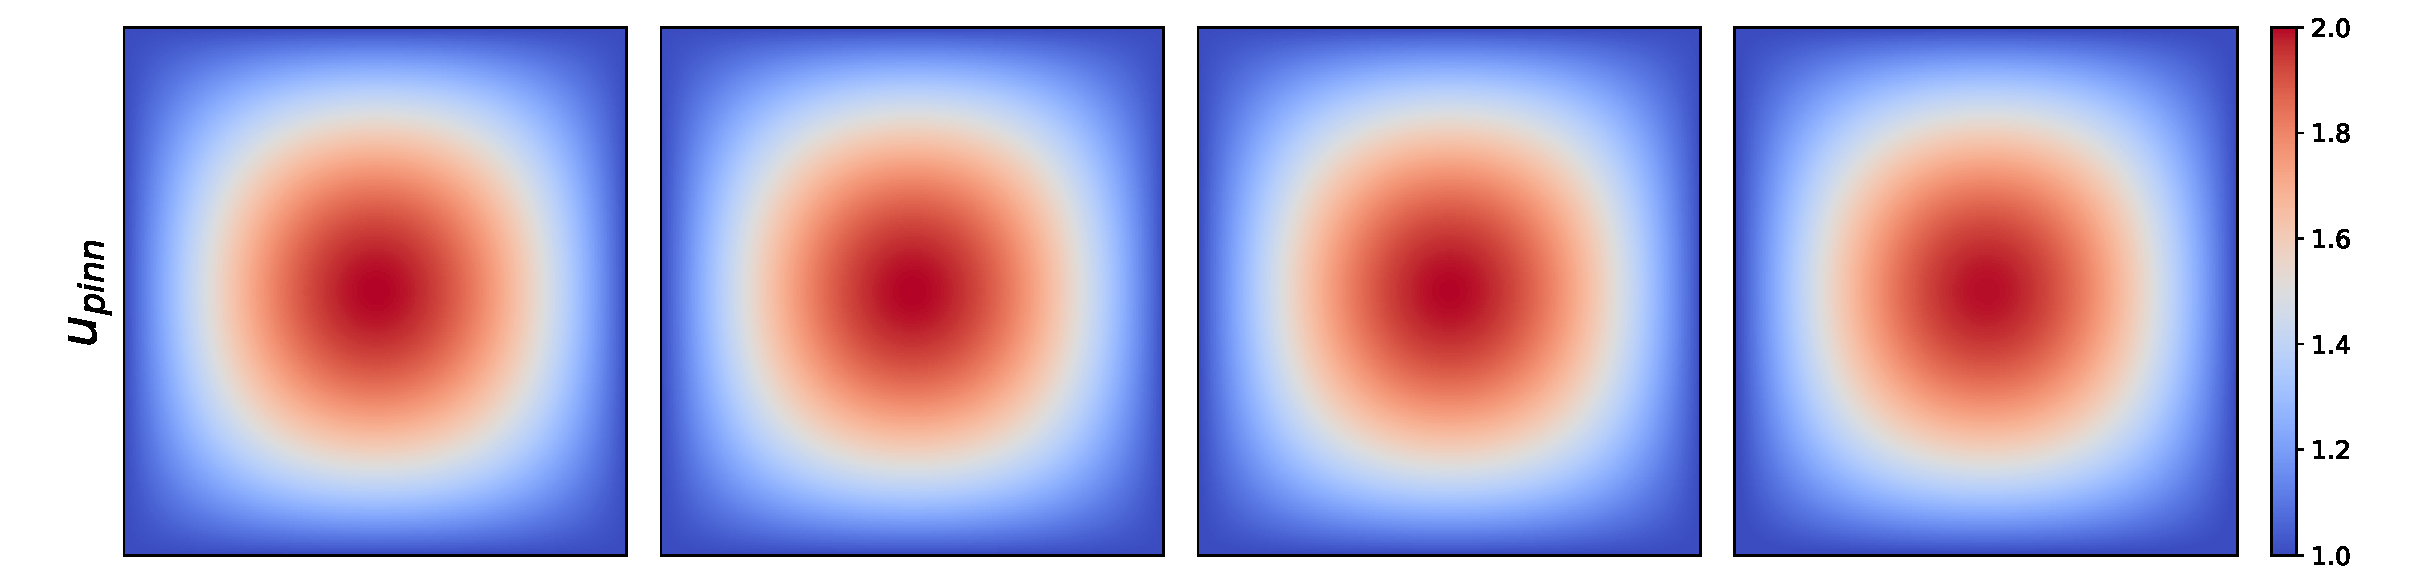
\includegraphics[width=\textwidth]{figures3/non_smooth_unn.eps}\par
% 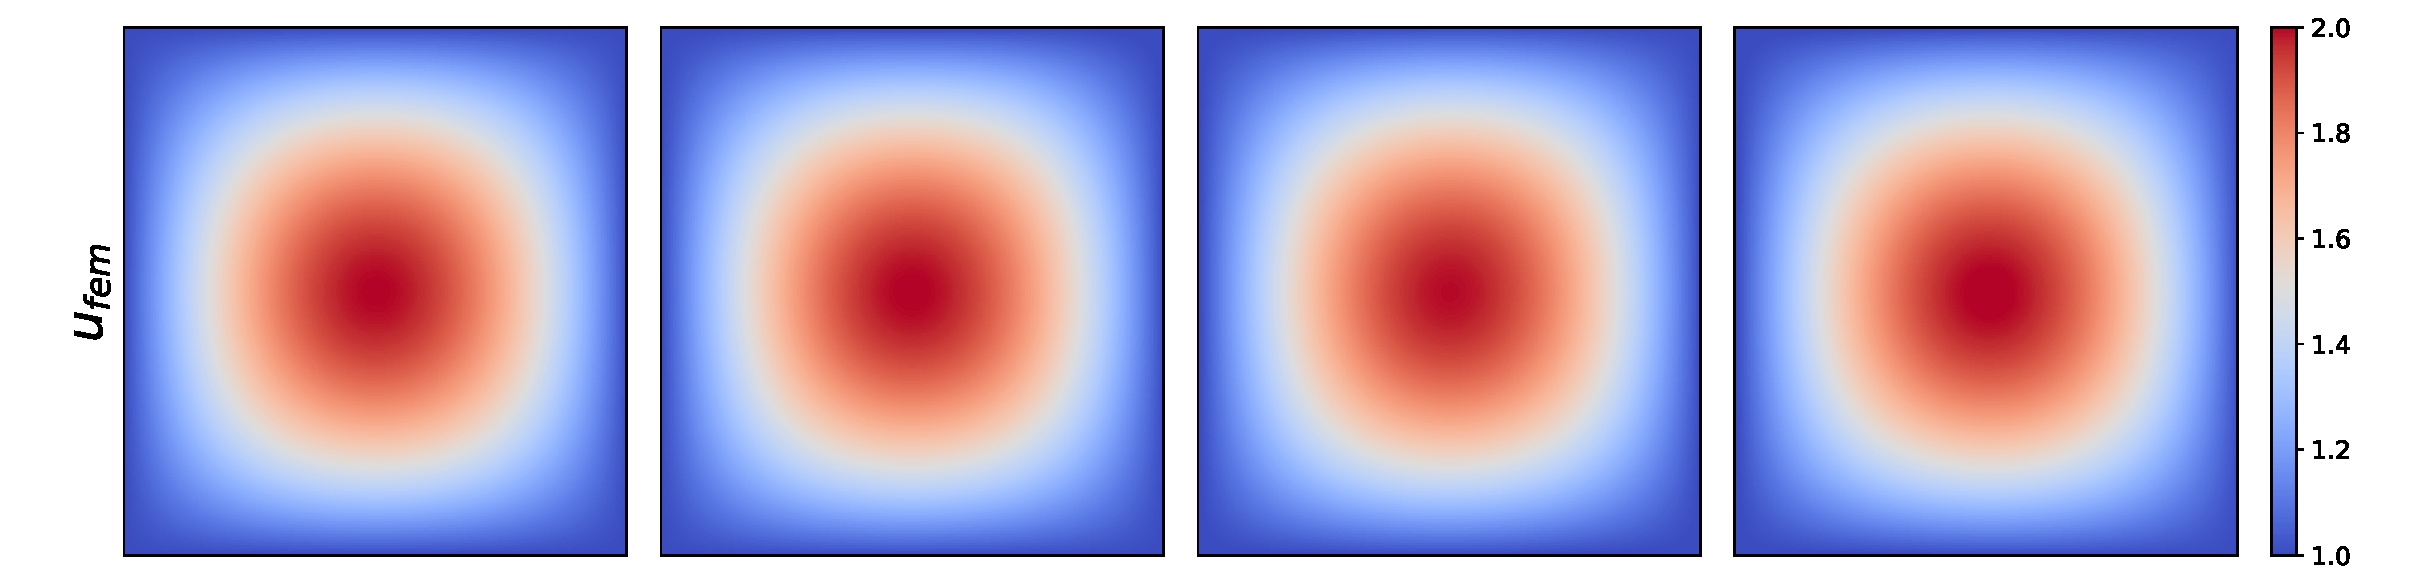
\includegraphics[width=\textwidth]{figures3/non_smooth_ufem.eps}\par
% 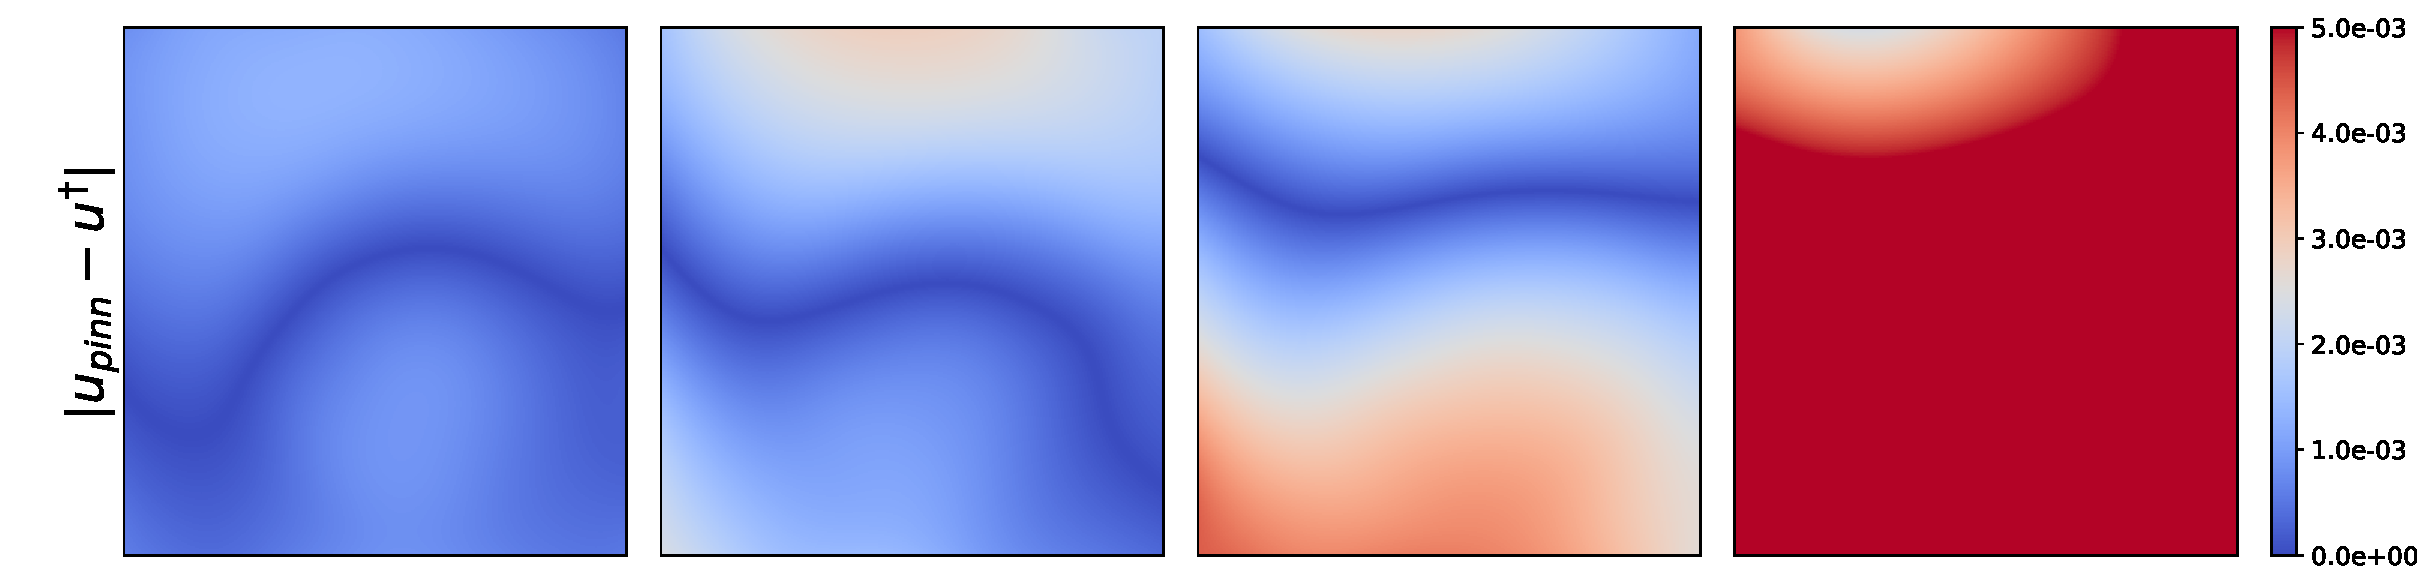
\includegraphics[width=\textwidth]{figures3/non_smooth_unn_err.eps}\par
% 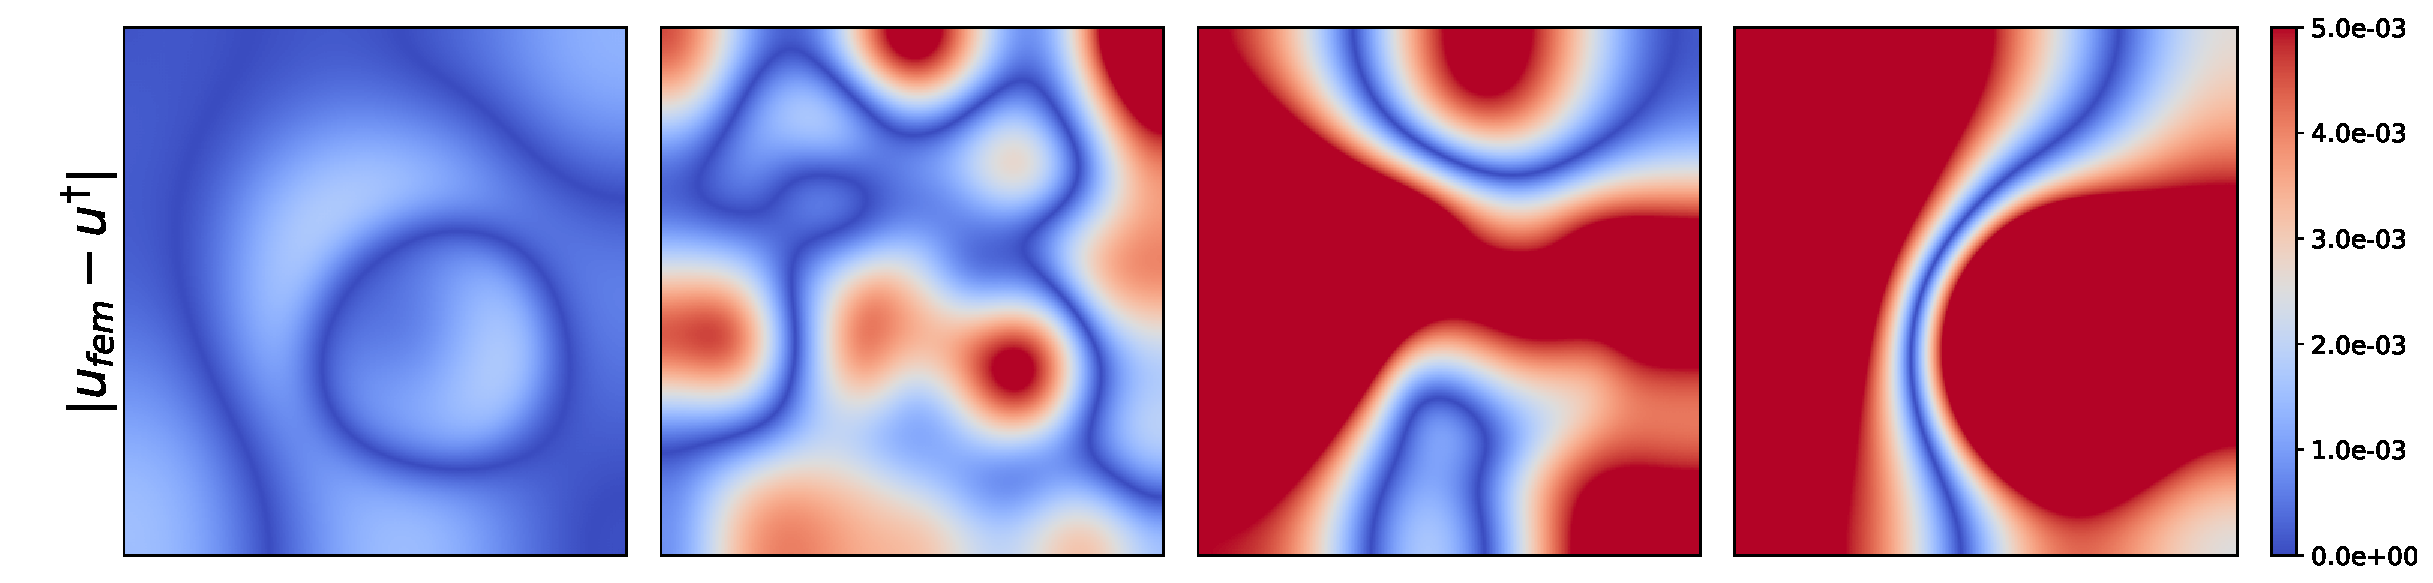
\includegraphics[width=\textwidth]{figures3/non_smooth_ufem_err.eps}
% \caption{从上到下依次为：Example \ref{example:nonsmooth} 中的真实势函数 $u^{\dagger}$，由 Tikhonov-PINNs 恢复的势函数 $u_{\text{pinn}}$，逐点绝对误差 $|u^{\dagger}-u_{\text{pinn}}|$，由 FEM 恢复的势函数 $u_{\text{fem}}$，逐点绝对误差 $|u^{\dagger}-u_{\text{fem}}|$。我们绘制了不同噪声水平下的结果。}
% \label{fig:example:nonsmooth:u}
% \end{figure}

% \begin{figure}[htbp]
% \centering
% \setlength{\abovecaptionskip}{10pt}
% 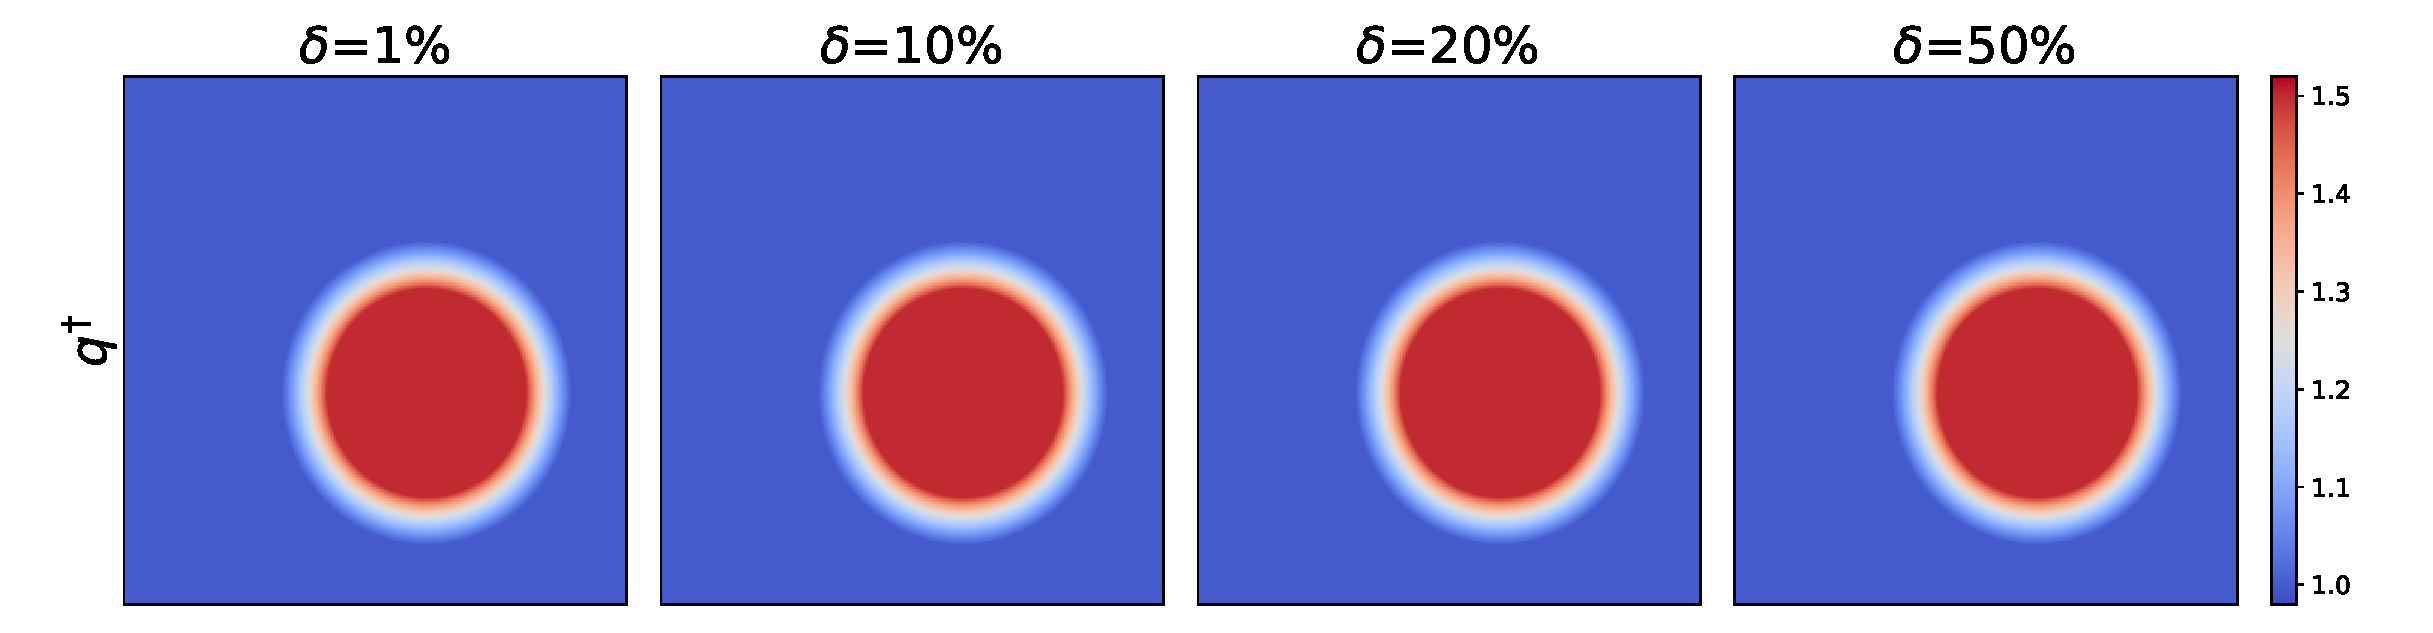
\includegraphics[width=\textwidth]{figures3/non_smooth_qdag.eps}\par
% 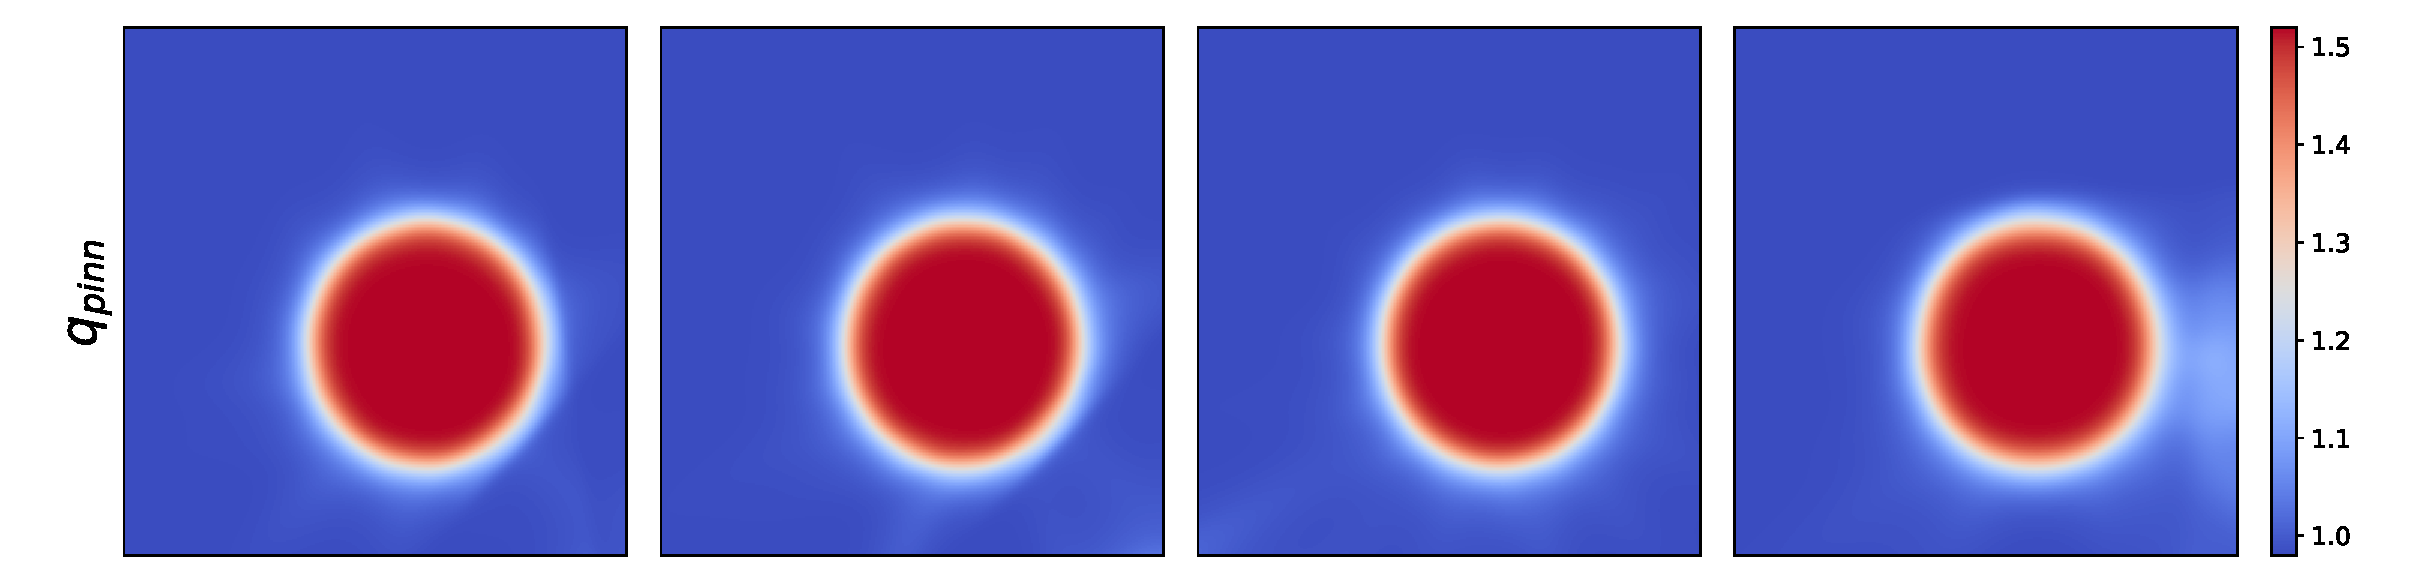
\includegraphics[width=\textwidth]{figures3/non_smooth_qnn.eps}\par
% 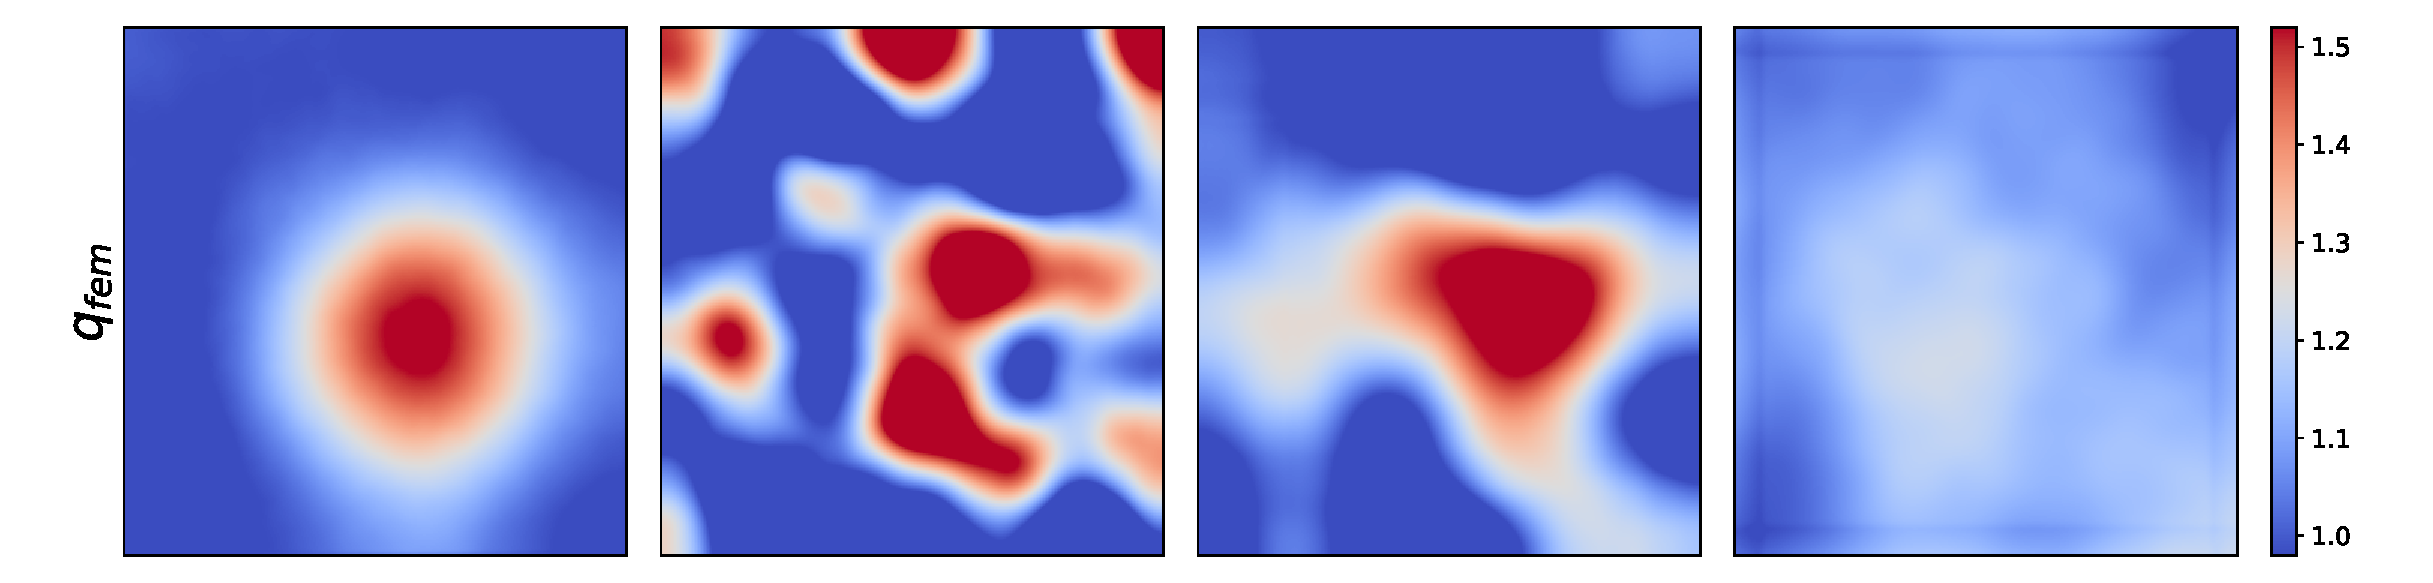
\includegraphics[width=\textwidth]{figures3/non_smooth_q_fem.eps}\par
% 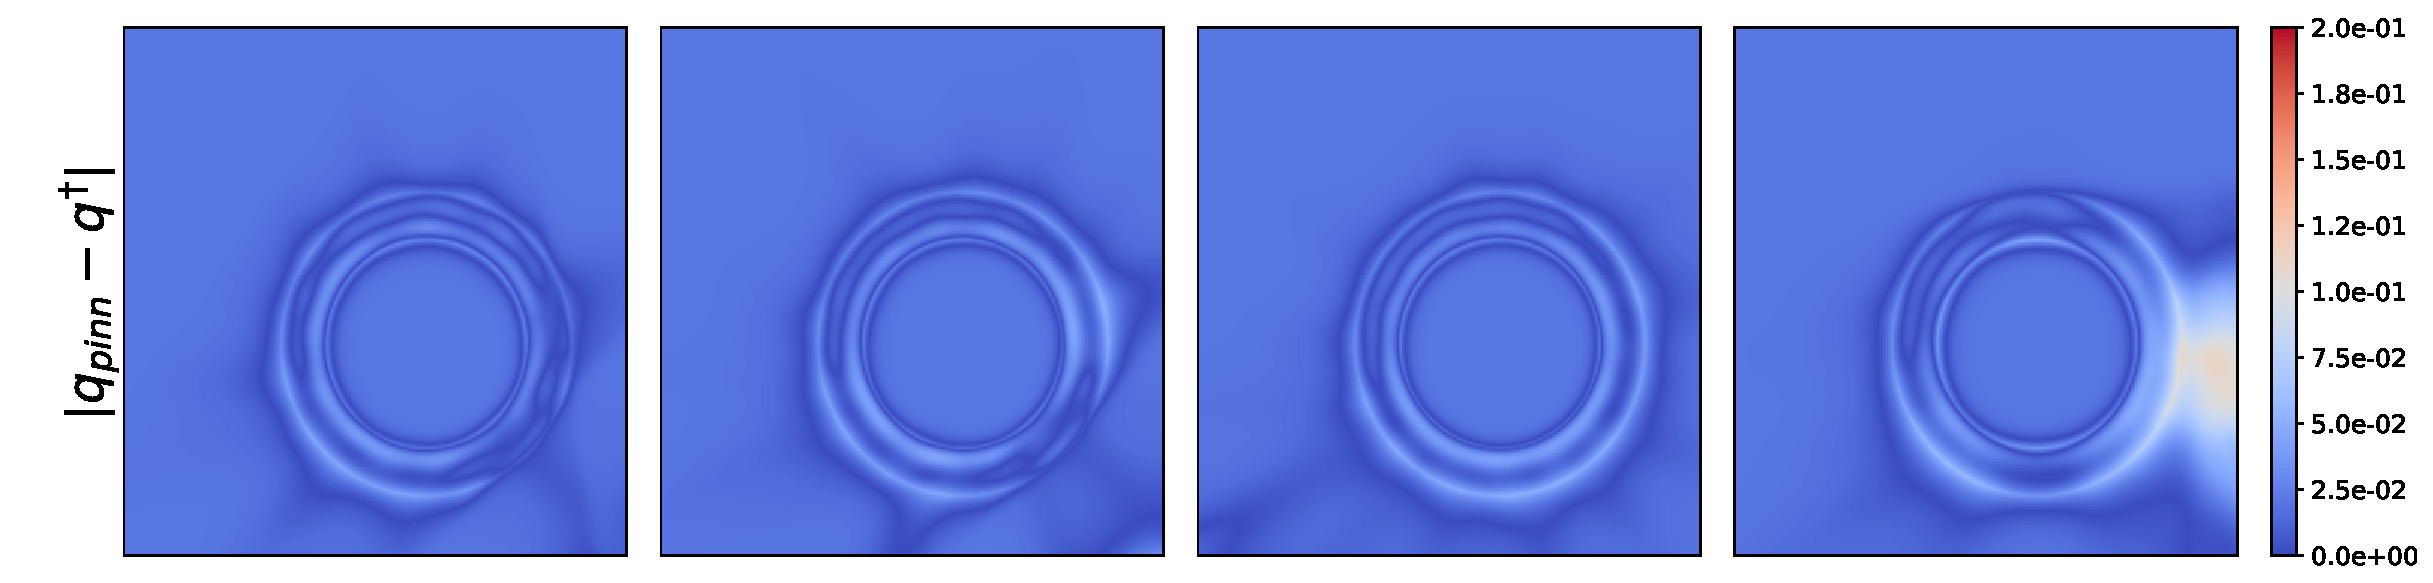
\includegraphics[width=\textwidth]{figures3/non_smooth_qnn_err.eps}\par
% 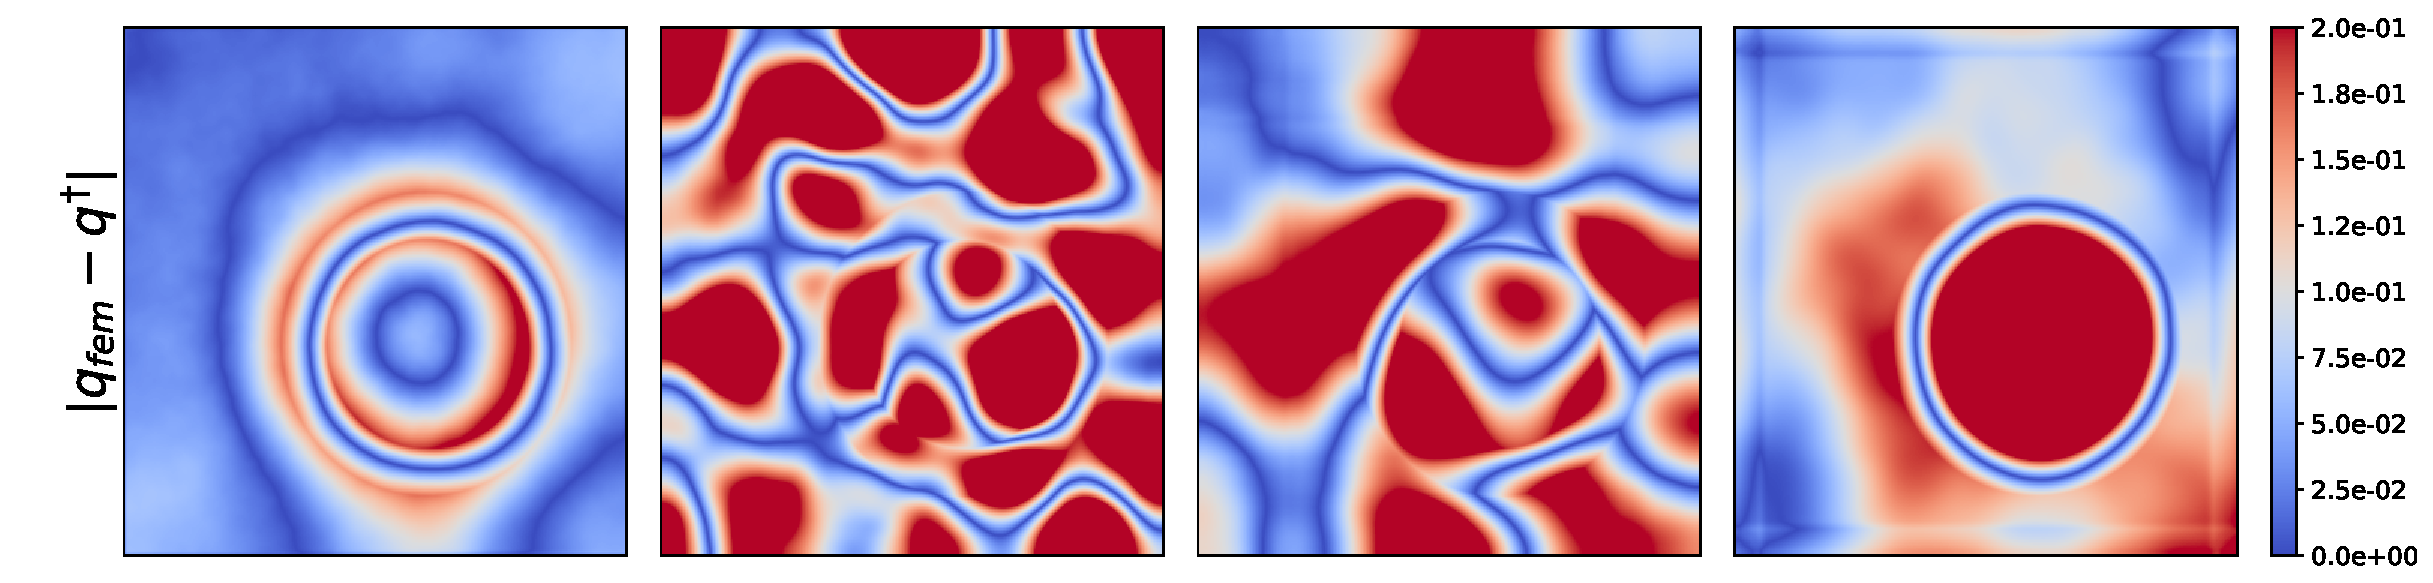
\includegraphics[width=\textwidth]{figures3/non_smooth_qfem_err.eps}
% \caption{从上到下依次为：Example \ref{example:nonsmooth} 中的真实势函数 $q^{\dagger}$，由 Tikhonov-PINNs 恢复的势函数 $q_{\text{pinn}}$，逐点绝对误差 $|q^{\dagger}-q_{\text{pinn}}|$，由 FEM 恢复的势函数 $q_{\text{fem}}$，逐点绝对误差 $|q^{\dagger}-q_{\text{fem}}|$。我们绘制了不同噪声水平下的结果。}
% \label{fig:example:nonsmooth}
% \end{figure}

% 在本例中，势函数 $q^{\dagger}$ 呈现出一种平台结构：它在红圈内部和蓝圈外部均保持常数。如图 \ref{fig:example:nonsmooth:u} 和图 \ref{fig:example:nonsmooth} 所示，重构 $u$ 相对简单，Tikhonov-PINNs 和基于有限元的方法均表现良好。然而，在重构 $q$ 时，Tikhonov-PINNs 成功捕捉到了常数值区域，而有限元方法未能精确识别 $q$ 中的界面，导致误差显著偏高。即使在高噪声水平下（例如 $\delta = 50\%$），我们的方法仍能恢复势函数的整体结构，而有限元方法几乎产生不了任何有意义的信息。

% \subsubsection{不连续问题}

% 作为第三个例子，我们将求解一个不连续势函数的反问题。
% \begin{example}\label{example:discontinuous}
% 令 $\Omega=(0,1)^{2}$ 且 $\alpha\equiv 1$。定义精确势函数 $q^{\dagger}$ 为：
% \begin{align*}
% \zeta(x_{1},x_{2})&=\exp\{-9\times(x_{1}-0.5)^{2}-9\times(x_{2}-0.5)^{2}\}, \\
% q^{\dagger}(x_{1},x_{2})&=1.0+0.5\times\zeta(x_{1},x_{2})\chi_{\{x_{1}\geq x_{2}\}},
% \end{align*}
% 精确解 $u^{\dagger}$ 为：$u^{\dagger}(x_{1},x_{2})=1+\sin(\pi x_{1})\sin(\pi x_{2})$。
% \end{example}

% \begin{table}[hbtp]
% \centering
% \footnotesize
% \caption{例 \ref{example:discontinuous} 中恢复的势函数 $\hat{q}$ 和解 $\hat{u}$ 的相对 $L^{2}$ 误差。}
% \begin{tabular}{lrrrrrr}
% \hline
% \multirow{2}[0]{*}{$\delta $ = 1\%} & \multicolumn{6}{c}{正则化参数 $\lambda$} \\
% \cline{2-7}
% & \multicolumn{1}{l}
% {$1.0\times 10^{-5}$} & 
% \multicolumn{1}{l}{$1.0\times 10^{-6}$} &
% \multicolumn{1}{l}{$1.0\times 10^{-7}$} &
% \multicolumn{1}{l}{$1.0\times 10^{-8}$} & 
%    \multicolumn{1}{l}{$1.0\times 10^{-9}$} & {0} \\
%    \hline
% $\text{err}(u_{\text{pinn}})$ & $2.05\times 10^{-3}$ & $1.54\times 10^{-3}$ & $1.07\times 10^{-3}$ & $9.83\times 10^{-4}$ & $7.55\times 10^{-4}$ & $6.42\times 10^{-4}$ \\
% $\text{err}(u_{\text{fem}})$&$1.46\times 10^{-3}$ & $7.05\times 10^{-4}$ & $4.80\times 10^{-4}$ & $2.66\times 10^{-4}$ & $2.50\times 10^{-4}$ & $2.38\times 10^{-4}$\\
% $\text{err}(q_{\text{pinn}})$ & $9.82\times 10^{-2}$ & $8.50\times 10^{-2}$ & $6.76\times 10^{-2}$ & $5.23\times 10^{-2}$ & $3.49\times 10^{-2}$ & \textbf{2.79$\times$ 10$^{-2}$} \\
% $\text{err}(q_{\text{fem}})$&$8.42\times 10^{-2}$ & $6.36\times 10^{-2}$ & $5.62\times 10^{-2}$ & $4.84\times 10^{-2}$ & $4.53\times 10^{-2}$ & $4.55\times 10^{-2}$\\
% \hline
% &       &       &       &       &       &  \\
% \hline
% \multirow{2}[0]{*}{$\delta$ = 10\%} & \multicolumn{6}{c}{正则化参数 $\lambda$} \\
% \cline{2-7}
% & $1.0\times 10^{-5}$ & $1.0\times 10^{-6}$ & $1.0\times 10^{-7}$ & $1.0\times 10^{-8}$ & $1.0\times 10^{-9}$ & \multicolumn{1}{r}{0} \\
% \hline
% $\text{err}(u_{\text{pinn}})$ & $1.96\times 10^{-3}$ & $1.74\times 10^{-3}$ & $1.38\times 10^{-3}$ & $1.12\times 10^{-3}$ & $1.49\times 10^{-3}$ & $1.48\times 10^{-3}$ \\
% $\text{err}(u_{\text{fem}})$&$1.80\times 10^{-3}$ & $9.42\times 10^{-4}$ & $1.42\times 10^{-3}$ & $1.53\times 10^{-3}$ & $1.69\times 10^{-3}$ & $1.97\times 10^{-3}$\\
% $\text{err}(q_{\text{pinn}})$ & $1.01\times 10^{-1}$ & $8.74\times 10^{-2}$ & $7.07\times 10^{-2}$ & \textbf{5.01$\times$ 10$^{-2}$} & $5.59\times 10^{-2}$ & $5.28\times 10^{-2}$ \\
% $\text{err}(q_{\text{fem}})$&$8.44\times 10^{-2}$ & $6.57\times 10^{-2}$ & $9.31\times 10^{-2}$ & $1.58\times 10^{-1}$ & $1.68\times 10^{-1}$ & $1.85\times 10^{-1}$\\
% \hline
% &       &       &       &       &       &  \\
% \hline
% \multirow{2}[0]{*}{$\delta = 20\%$} & \multicolumn{6}{c}{正则化参数 $\lambda$} \\
% \cline{2-7}
% & $1.0\times 10^{-5}$ & $1.0\times 10^{-6}$ & $1.0\times 10^{-7}$ & $1.0\times 10^{-8}$ & $1.0\times 10^{-9}$ & \multicolumn{1}{r}{0} \\
% \hline
% $\text{err}(u_{\text{pinn}})$ & $2.65\times 10^{-3}$ & $2.07\times 10^{-3}$ & $1.78\times 10^{-3}$ & $1.60\times 10^{-3}$ & $1.75\times 10^{-3}$ & $1.87\times 10^{-3}$ \\
% $\text{err}(u_{\text{fem}})$&$1.74\times 10^{-3}$ & $2.18\times 10^{-3}$ & $4.48\times 10^{-3}$ & $3.91\times 10^{-3}$ & $4.67\times 10^{-3}$ & $3.08\times 10^{-3}$\\
% $\text{err}(q_{\text{pinn}})$ & $1.05\times 10^{-1}$ & $9.18\times 10^{-2}$ & $7.22\times 10^{-2}$ & \textbf{6.50$\times$ 10$^{-2}$} & $7.20\times 10^{-2}$ & $7.73\times 10^{-2}$ \\
% $\text{err}(q_{\text{fem}})$&$8.58\times 10^{-2}$ & $9.39\times 10^{-2}$ & $2.35\times 10^{-1}$ & $2.00\times 10^{-1}$ & $6.43\times 10^{-1}$ & $1.89\times 10^{-1}$\\
% \hline
% &       &       &       &       &       &  \\
% \hline
% \multirow{2}[0]{*}{$\delta = 50\%$} & \multicolumn{6}{c}{正则化参数 $\lambda$} \\
% \cline{2-7}
% & $1.0\times 10^{-5}$ & $1.0\times 10^{-6}$ & $1.0\times 10^{-7}$ & $1.0\times 10^{-8}$ & $1.0\times 10^{-9}$ & \multicolumn{1}{r}{0} \\
% \hline
% $\text{err}(u_{\text{pinn}})$ & $3.92\times 10^{-3}$ & $4.57\times 10^{-3}$ & $4.33\times 10^{-3}$ & $4.23\times 10^{-3}$ & $4.21\times 10^{-3}$ & $4.35\times 10^{-3}$ \\
% $\text{err}(u_{\text{fem}})$&$4.99\times 10^{-3}$ & $7.18\times 10^{-3}$ & $8.53\times 10^{-3}$ & $8.25\times 10^{-3}$ & $1.29\times 10^{-2}$ & $1.01\times 10^{-2}$\\
% $\text{err}(q_{\text{pinn}})$ & $1.21\times 10^{-1}$ & $1.04\times 10^{-1}$ & $8.50\times 10^{-2}$ & $8.08\times 10^{-2}$ & \textbf{8.04$\times$ 10$^{-2}$} & $1.06\times 10^{-1}$ \\
% $\text{err}(q_{\text{fem}})$&$1.08\times 10^{-1}$ & $2.27\times 10^{-1}$ & $5.12\times 10^{-1}$ & $4.62\times 10^{-1}$ & $5.90\times 10^{-1}$ & $8.28\times 10^{-1}$\\
% \hline
% \end{tabular}
% \label{tab:discontinuous}
% \end{table}

% \begin{figure}[htbp]
% \centering
% \setlength{\abovecaptionskip}{10pt}
% 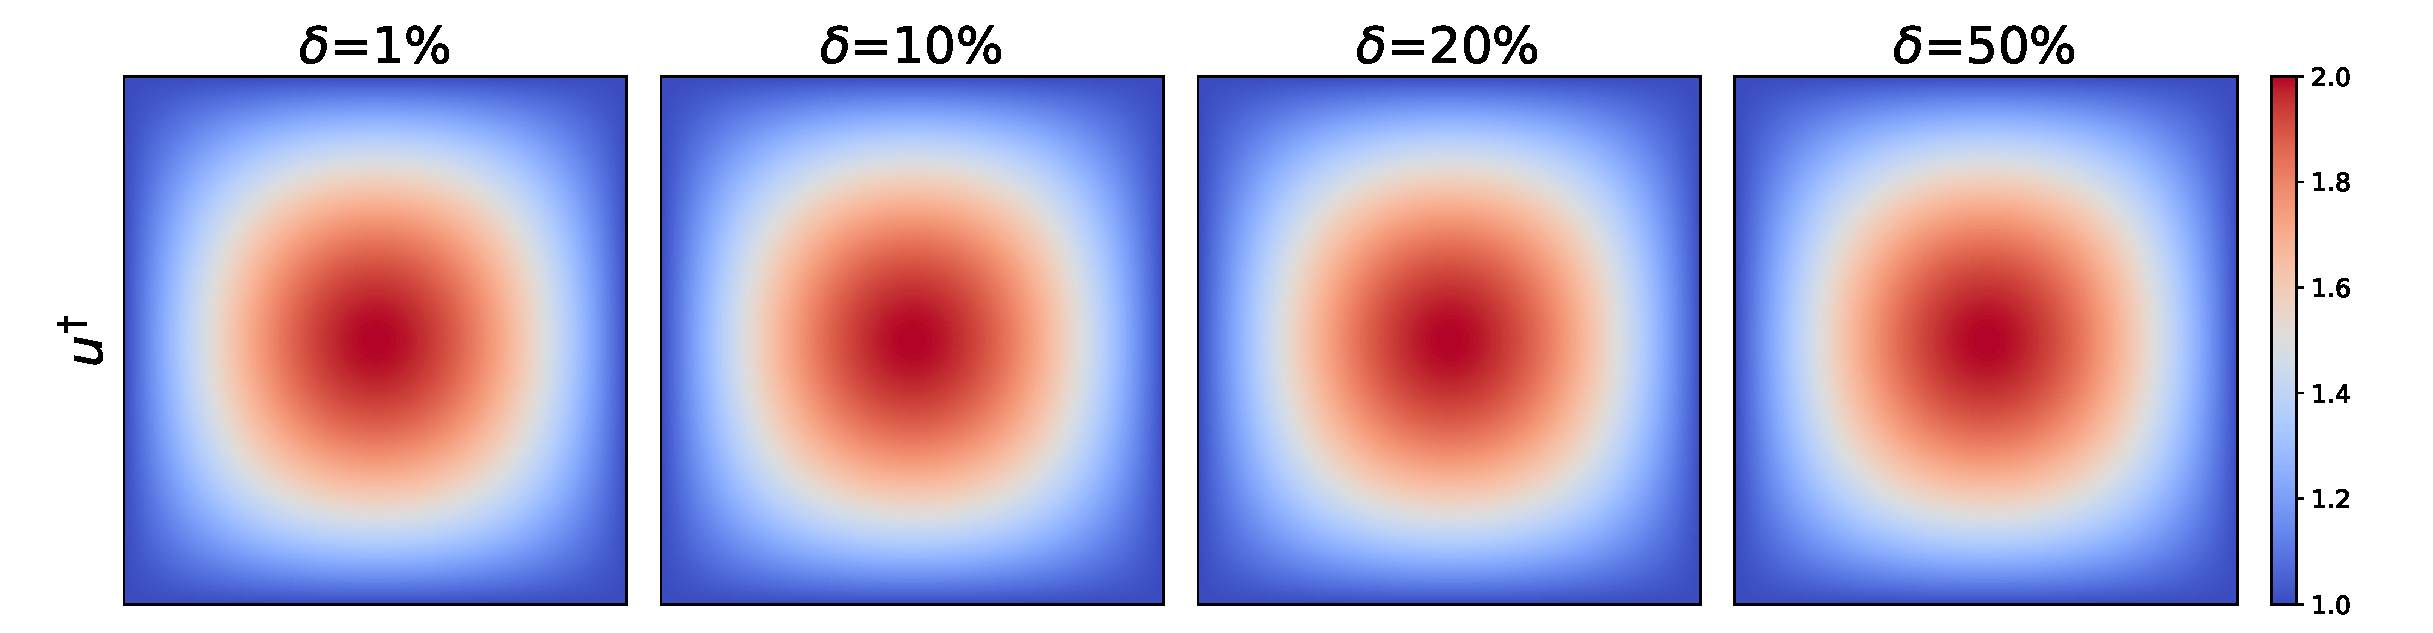
\includegraphics[width=\textwidth]{figures3/discontinuous_udag.eps}\par
% 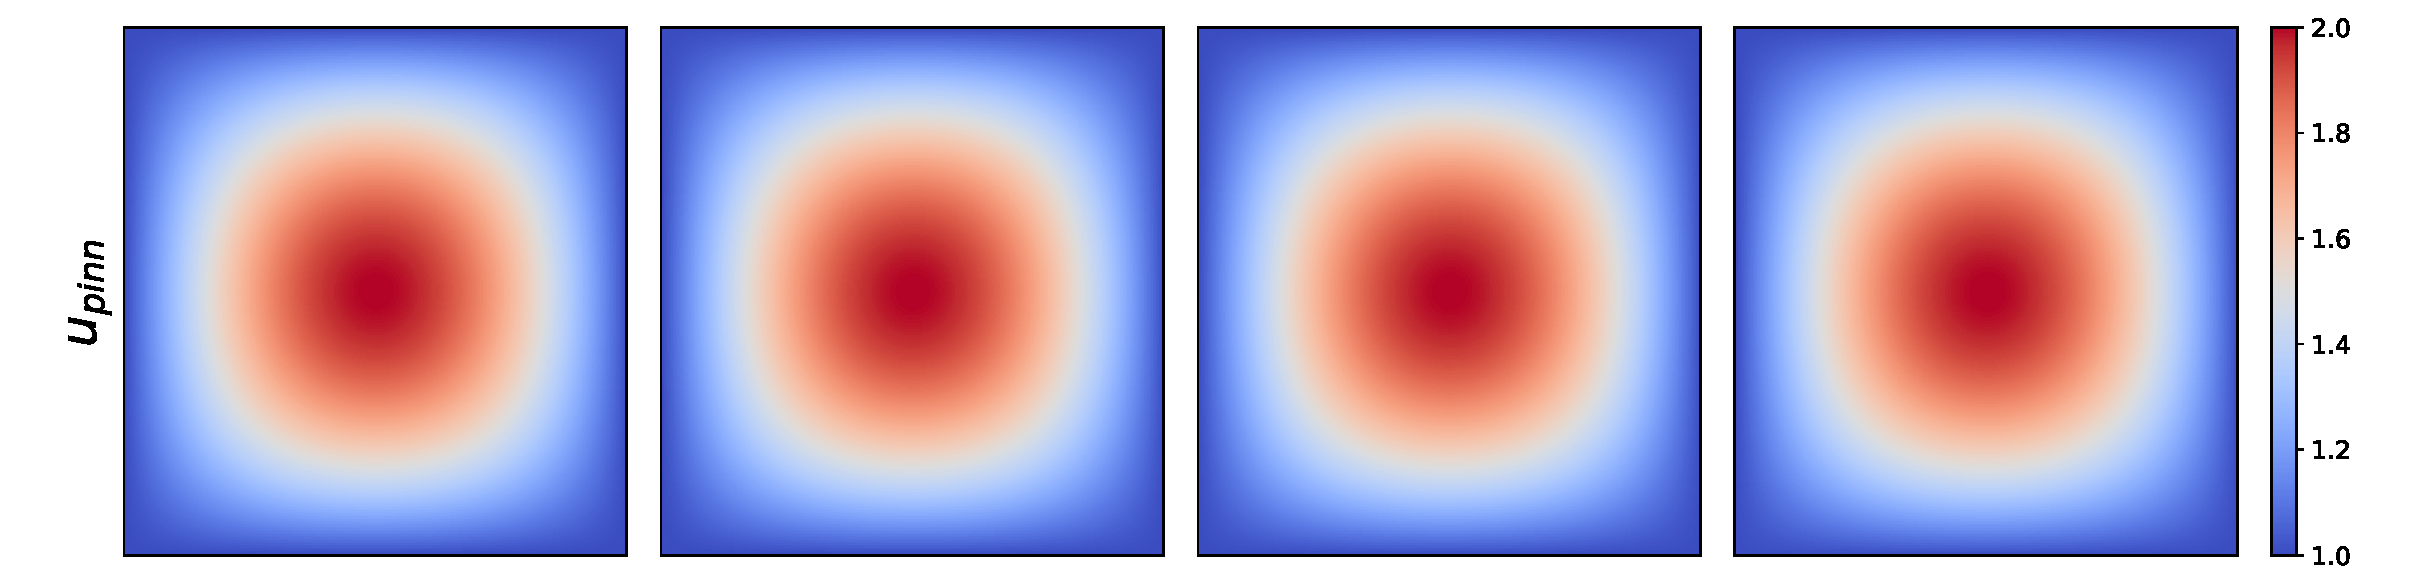
\includegraphics[width=\textwidth]{figures3/discontinuous_unn.eps}\par
% 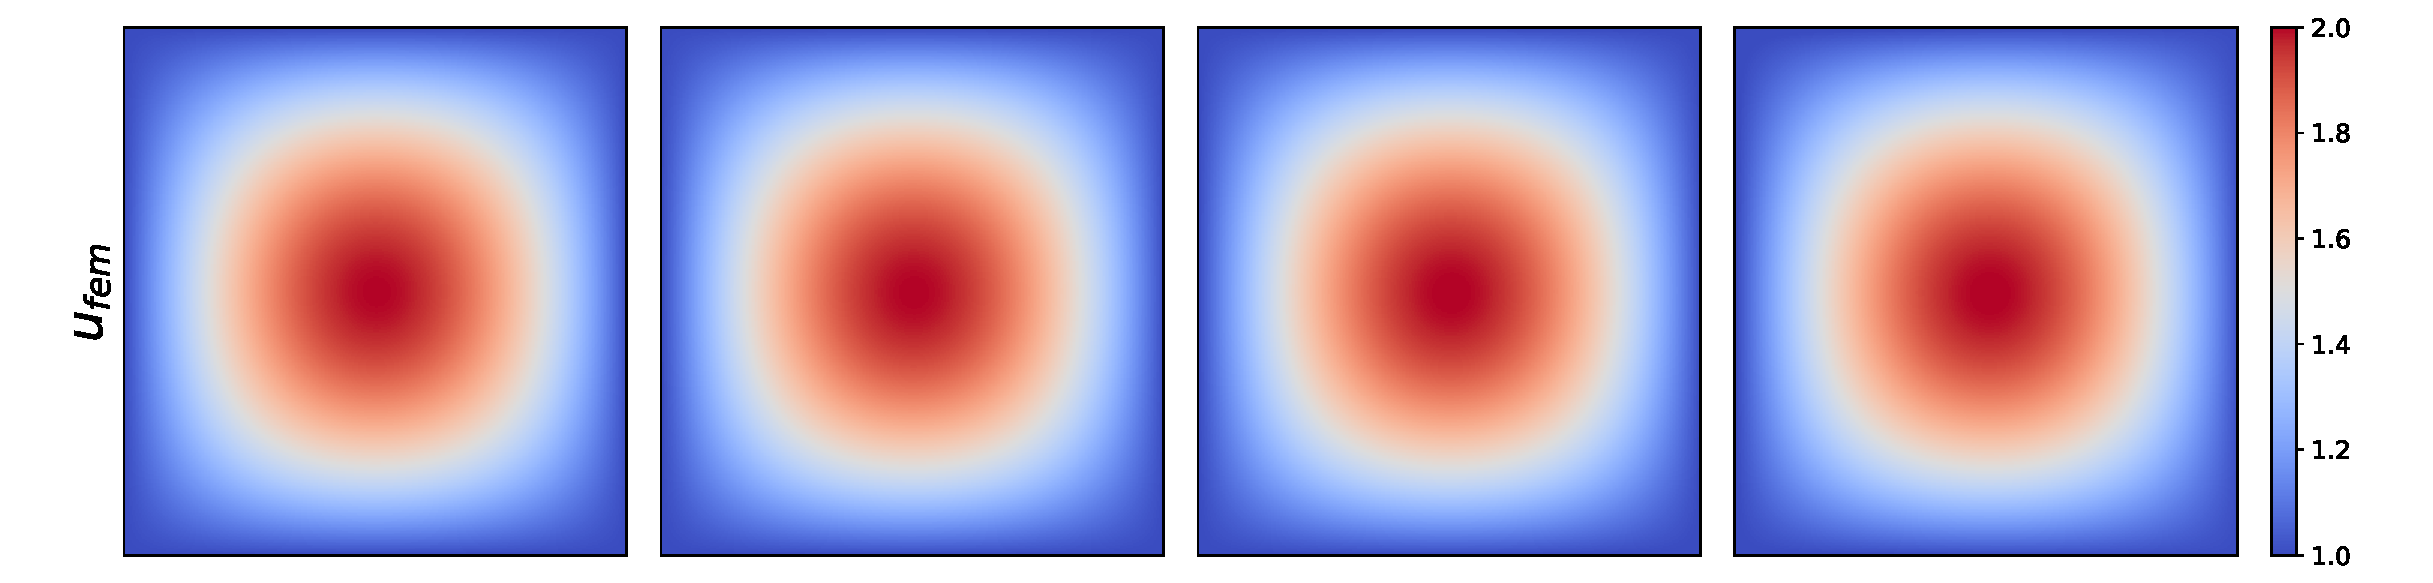
\includegraphics[width=\textwidth]{figures3/discontinuous_ufem.eps}\par
% 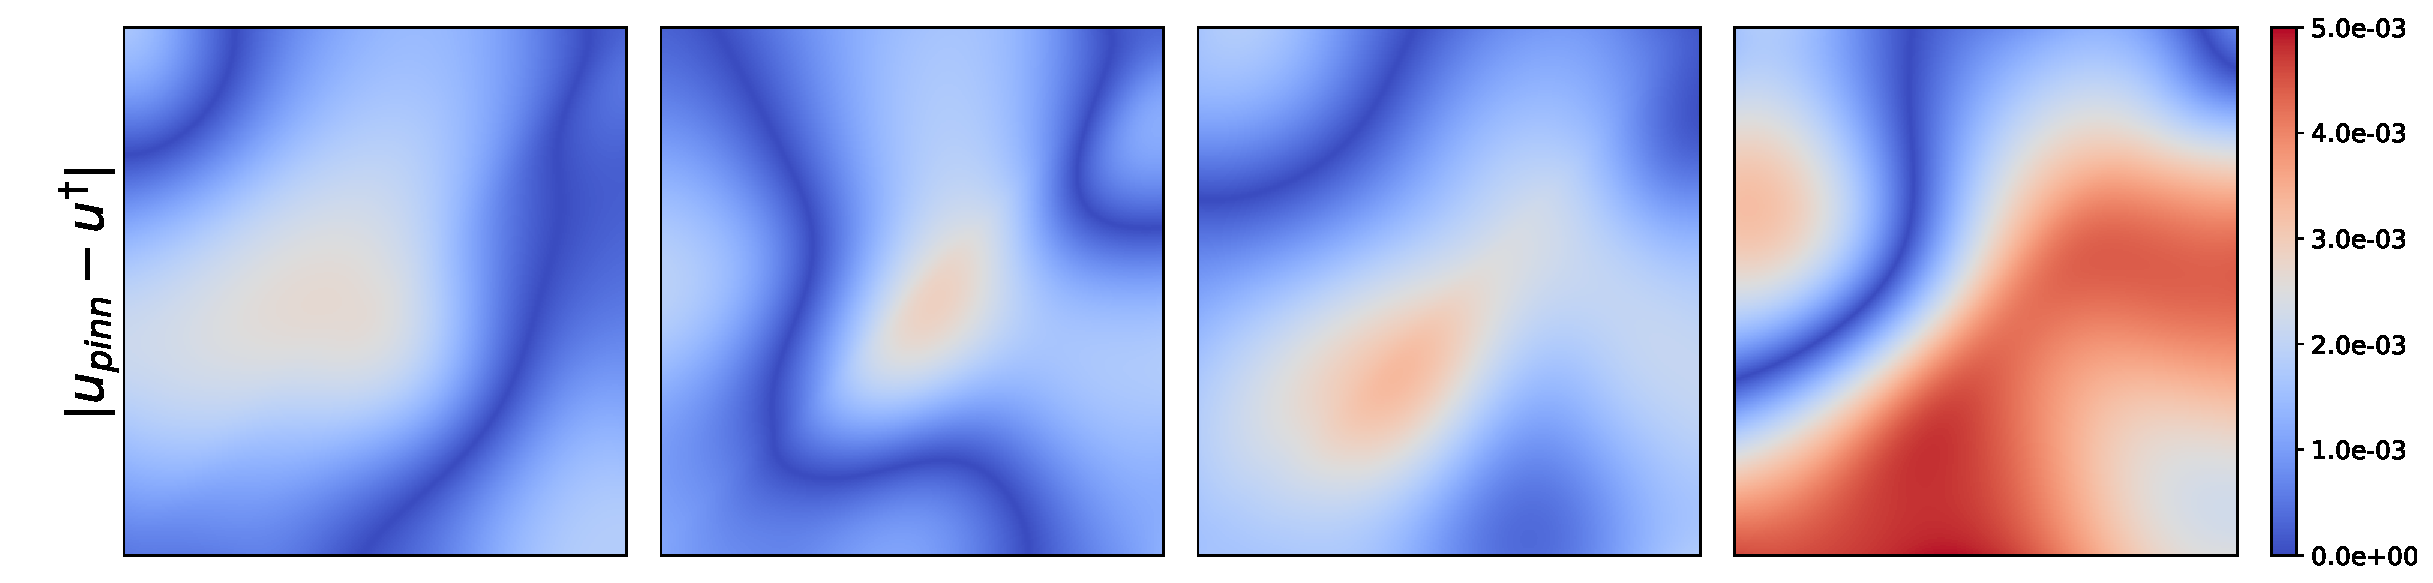
\includegraphics[width=\textwidth]{figures3/discontinuous_unn_err.eps}\par
% 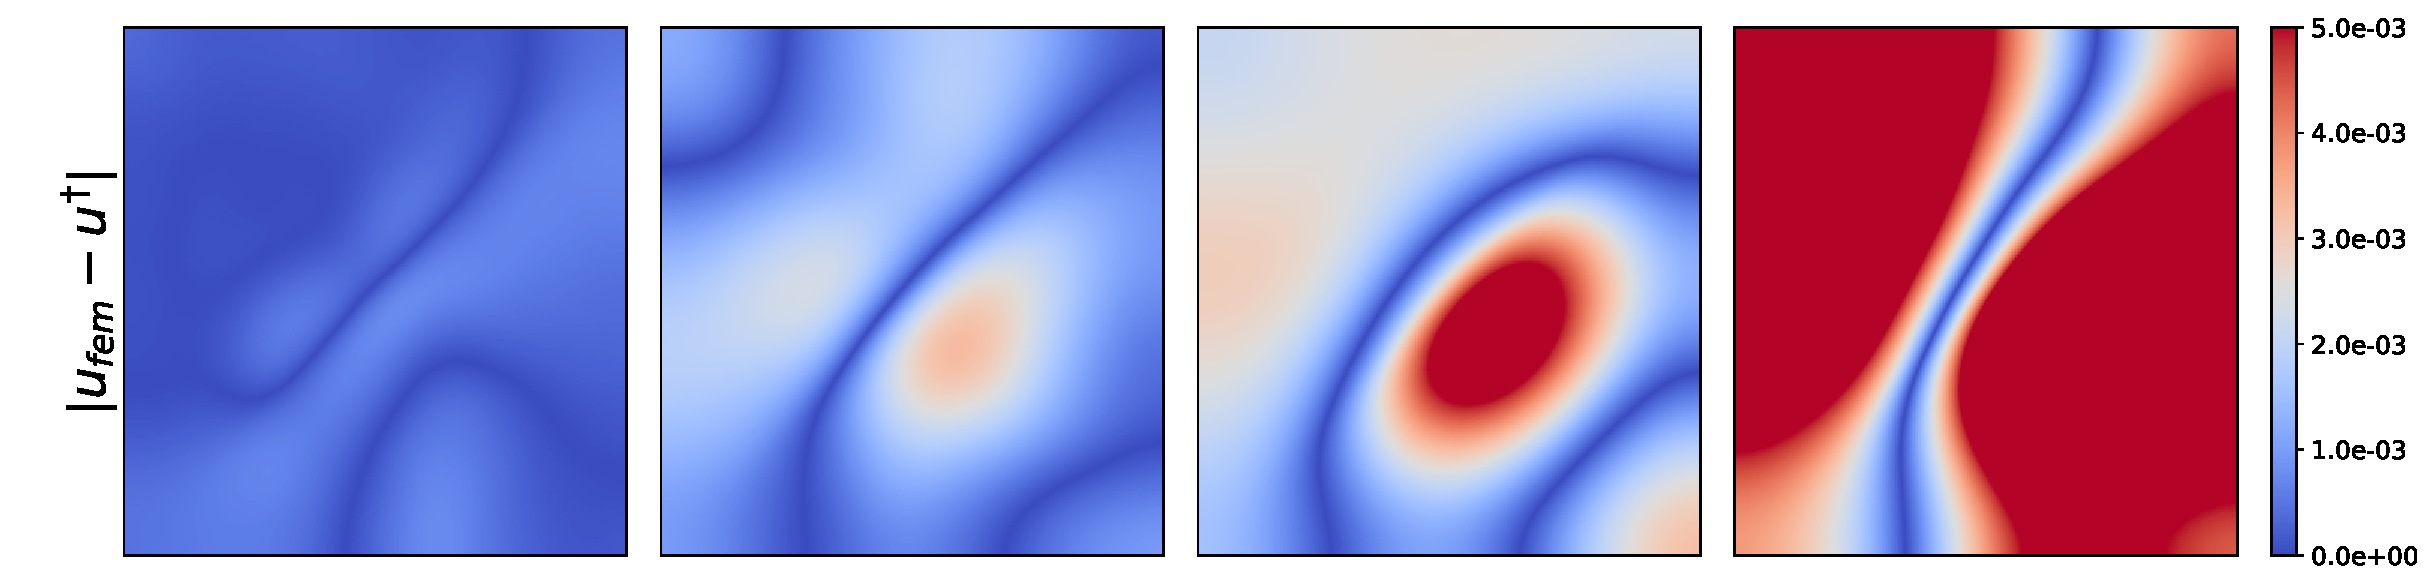
\includegraphics[width=\textwidth]{figures3/discontinuous_ufem_err.eps}
% \caption{从上到下依次为：例 \ref{example:discontinuous} 中的真实解 $u^{\dagger}$，Tikhonov-PINNs 恢复的解 $u_{\text{pinn}}$，逐点绝对误差 $|u^{\dagger}-u_{\text{pinn}}|$，FEM 恢复的解 $u_{\text{fem}}$，以及逐点绝对误差 $|u^{\dagger}-u_{\text{fem}}|$。我们绘制了在不同噪声水平下的结果。}
% \label{fig:example:discontinuous:u}
% \end{figure}

% \begin{figure}[htbp]
% \centering
% \setlength{\abovecaptionskip}{10pt}
% 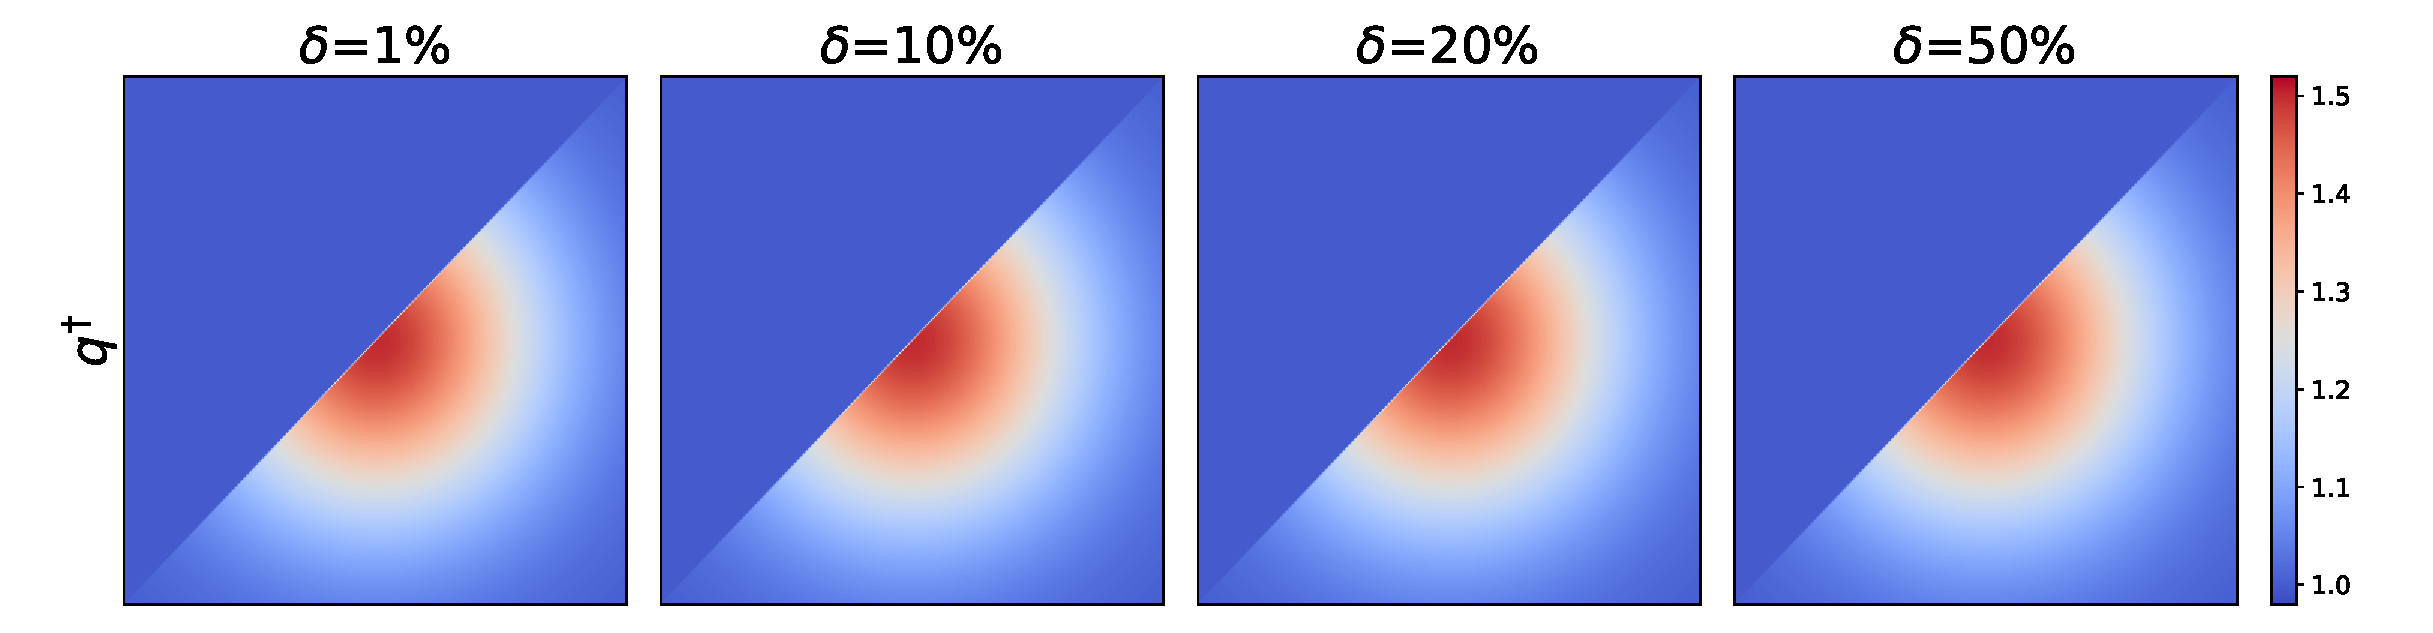
\includegraphics[width=\textwidth]{figures3/discontinuous_qdag.eps}\par
% 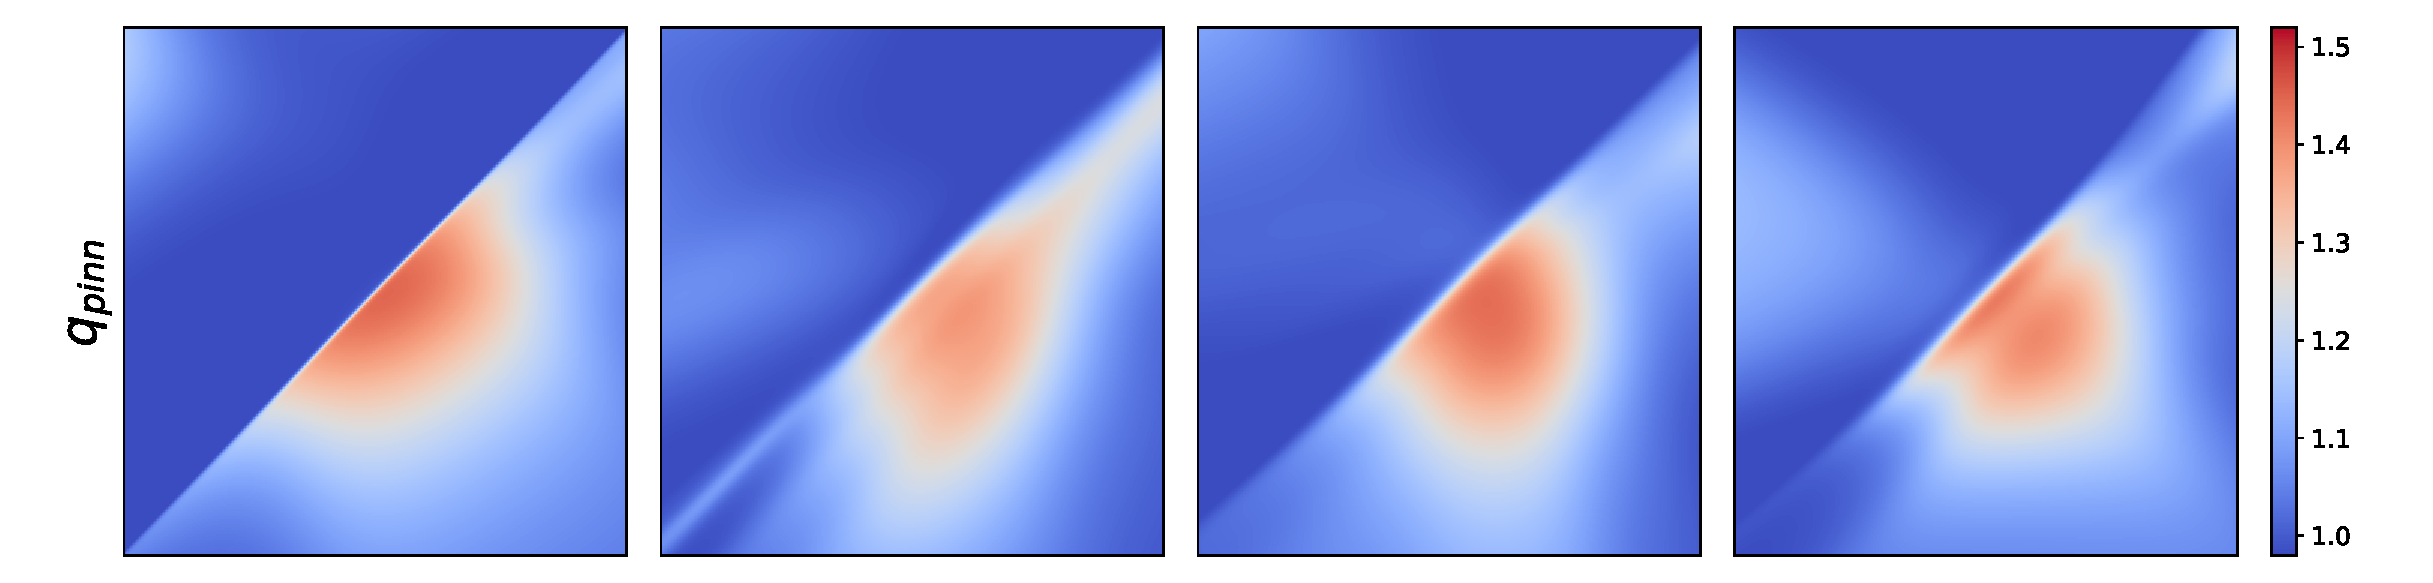
\includegraphics[width=\textwidth]{figures3/discontinuous_qnn.eps}\par
% 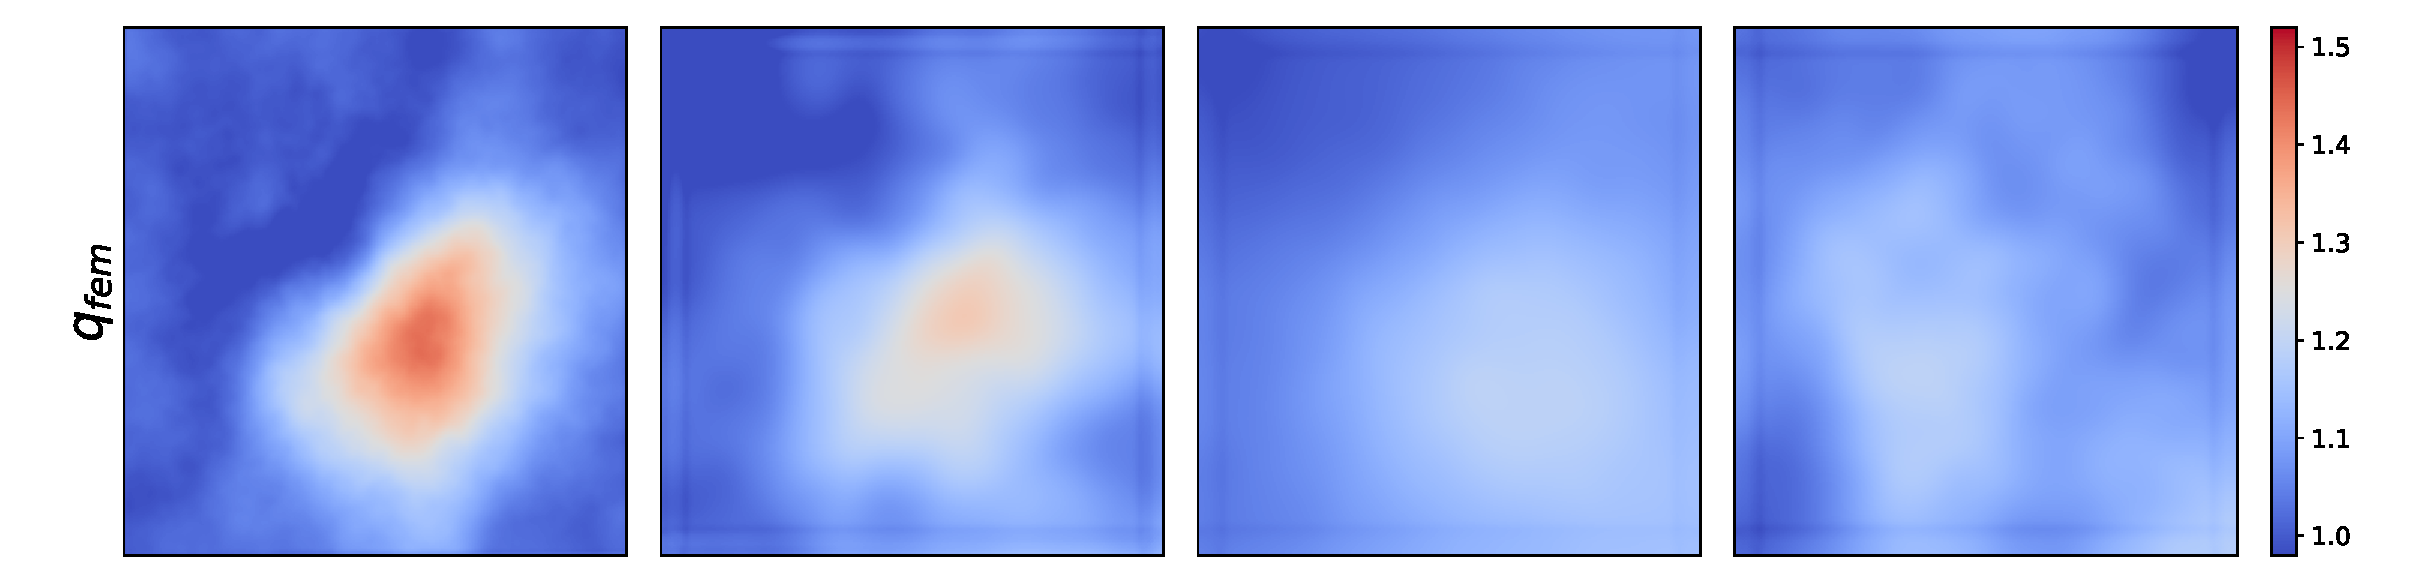
\includegraphics[width=\textwidth]{figures3/discontinuous_q_fem.eps}\par
% 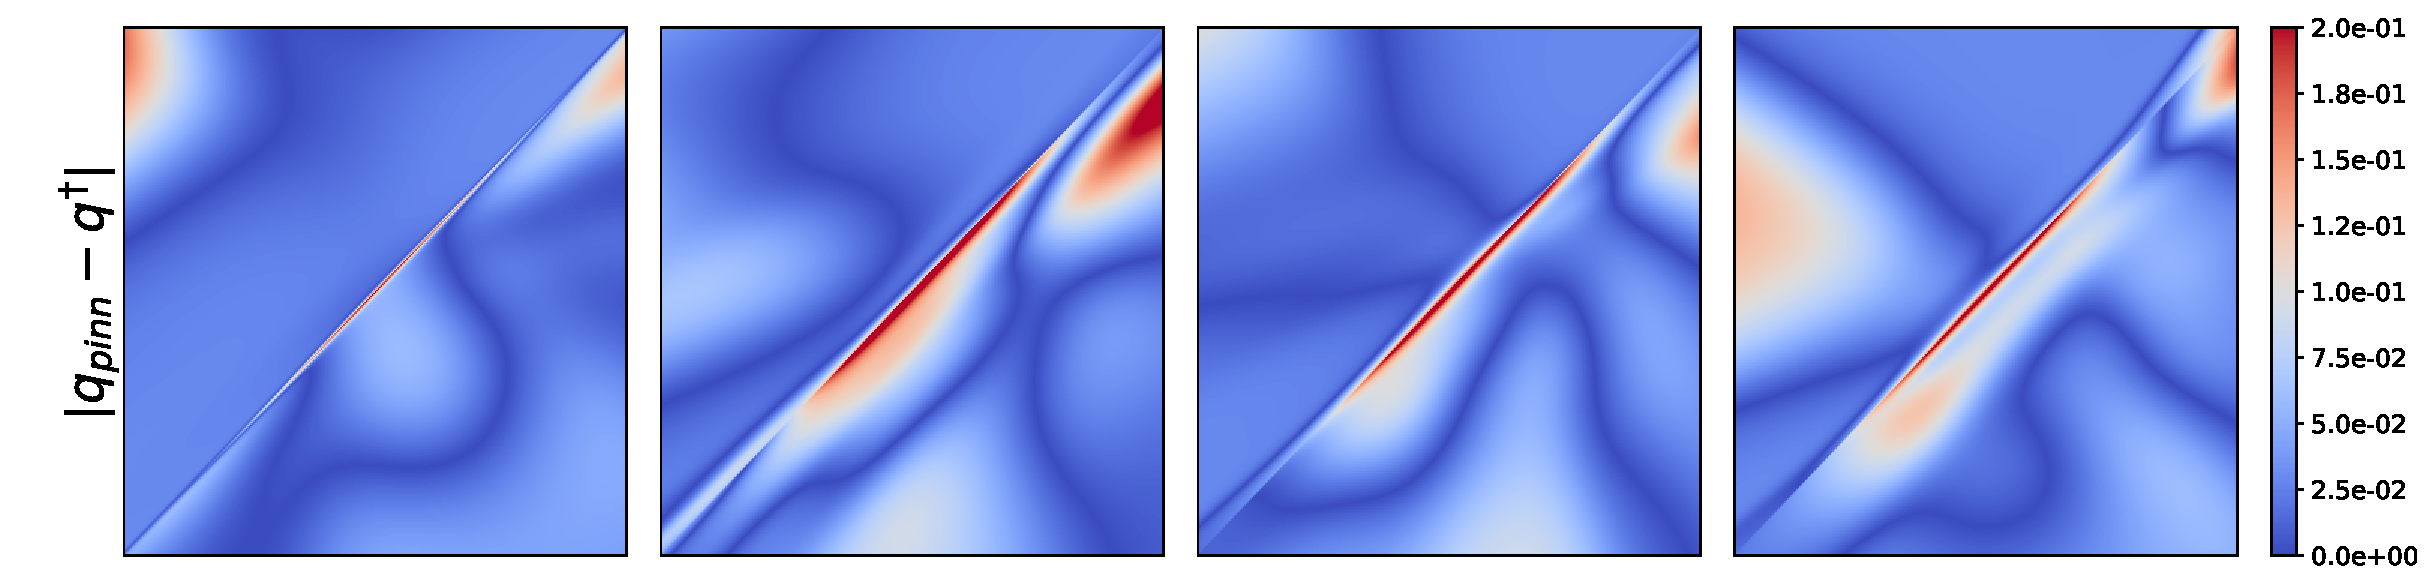
\includegraphics[width=\textwidth]{figures3/discontinuous_qnn_err.eps}\par
% 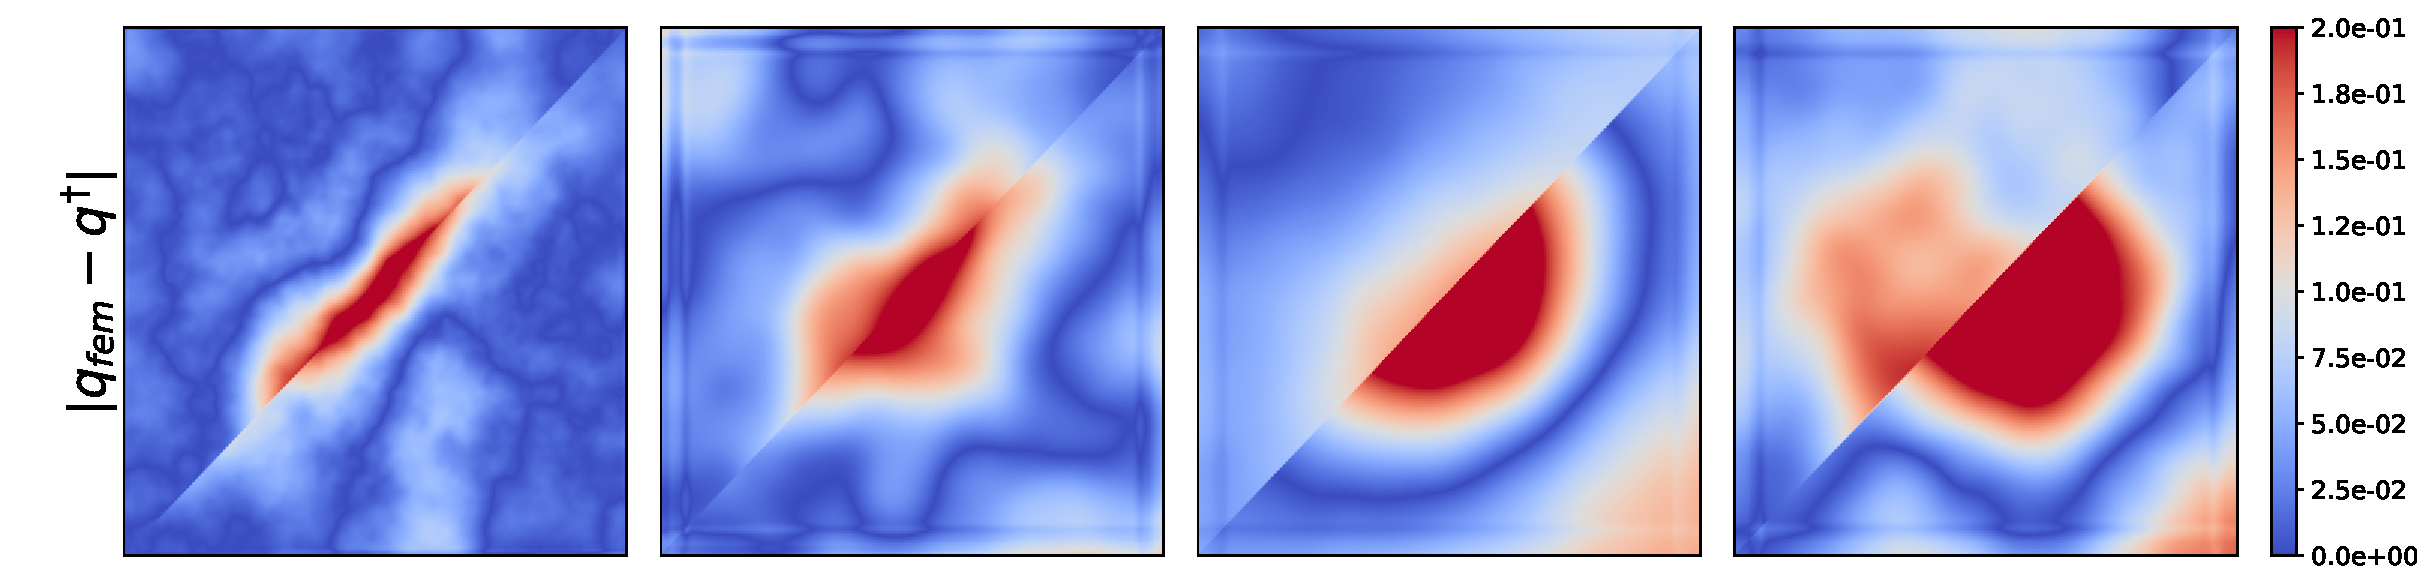
\includegraphics[width=\textwidth]{figures3/discontinuous_qfem_err.eps}
% \caption{从上到下依次为：例 \ref{example:discontinuous} 中的真实势函数 $q^{\dagger}$，Tikhonov-PINNs 恢复的势函数 $q_{\text{pinn}}$，逐点绝对误差 $|q^{\dagger}-q_{\text{pinn}}|$，FEM 恢复的势函数 $q_{\text{fem}}$，以及逐点绝对误差 $|q^{\dagger}-q_{\text{fem}}|$。我们绘制了在不同噪声水平下的结果。}
% \label{fig:example:discontinuous}
% \end{figure}

% 根据构造，势函数 $q$ 沿对角线 $x=y$ 呈现不连续性，这进一步加剧了反问题的不适定性。如图~\ref{fig:example:discontinuous:u} 和图~\ref{fig:example:discontinuous} 所示，Tikhonov-PINNs 能够在所有噪声水平下捕捉到这种不连续性。相比之下，有限元方法无法识别不连续区域，仅能在 1\% 的噪声水平下粗略定位高势区域。如表 \ref{tab:discontinuous} 所示，Tikhonov-PINNs 在所有噪声水平下对 $q$ 的相对误差均达到 $\calO(10^{-2})$ 左右，通常比有限元方法优越一个数量级。

% 还应注意，在上述实验中，当 $\lambda$ 非零时，Tikhonov-PINNs 通常能获得最优解（参见表 \ref{tab:discontinuous}）。这一观察结果部分说明了损失函数中的 Tikhonov 正则化对于提升标准 PINNs 方法的性能至关重要。

% \subsection{高维问题}
% 由于其无网格的特性，基于神经网络的方法可以很容易地扩展到高维问题，并在一定程度上缓解维数灾难。在本小节中，依照 \cite{jin2023conductivity} 中算例 5.4 的设置，我们将 Tikhonov-PINNs 应用于一个五维问题，这是传统有限元方法难以实现的场景。

% \begin{example}\label{example:highdim}
% 令 $\Omega=(0,1)^{5}$ 且 $\alpha\equiv 1$。我们考虑识别如下势函数：
% \begin{equation*}
% \begin{array}{rcl}
% q^{\dagger}(x)&=&1-(x_1-0.5)^2-(x_2-0.5)^2\\
% &{}&+\cos(\pi(x_3+1.5))+\cos(\pi (x_4+1.5))+\cos(\pi (x_5+1.5)),
% \end{array}
% \end{equation*}
% 准确解 $u^{\dagger}$ 为 $u^{\dagger}(x)=\sum_{i=1}^{5}(x_{i}+\frac{1}{3}x_{i}^3)$。
% \end{example}


% \begin{figure}
% \centering
% \setlength{\abovecaptionskip}{10pt}
% 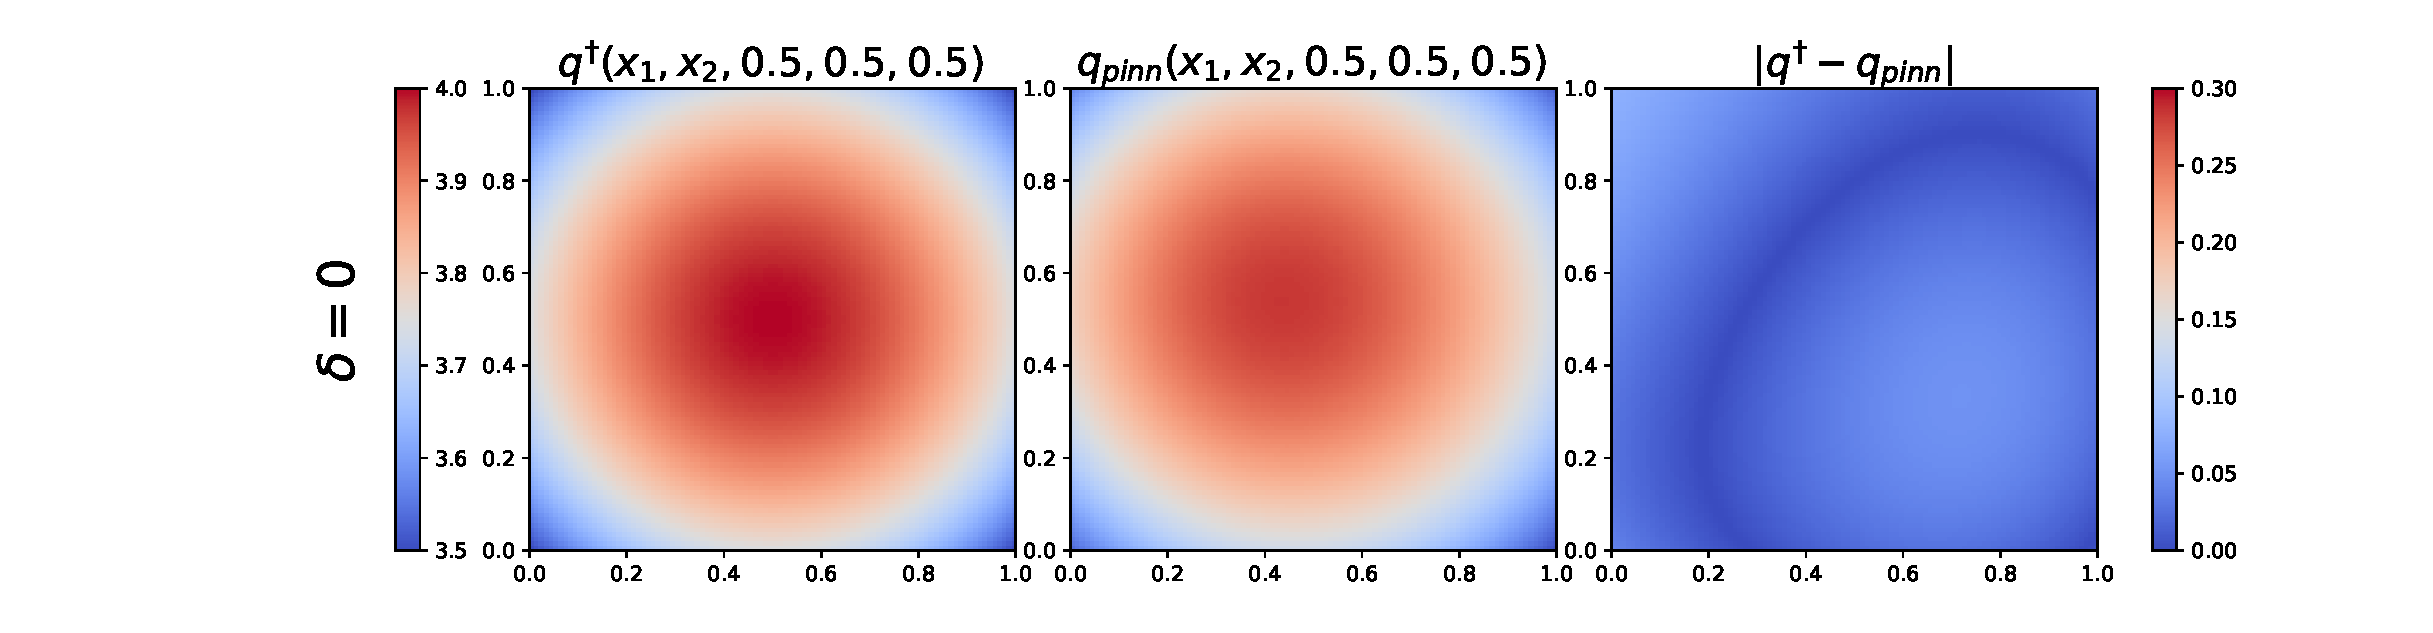
\includegraphics[width=\textwidth]{figures3/ex_5_00.eps}\par
% 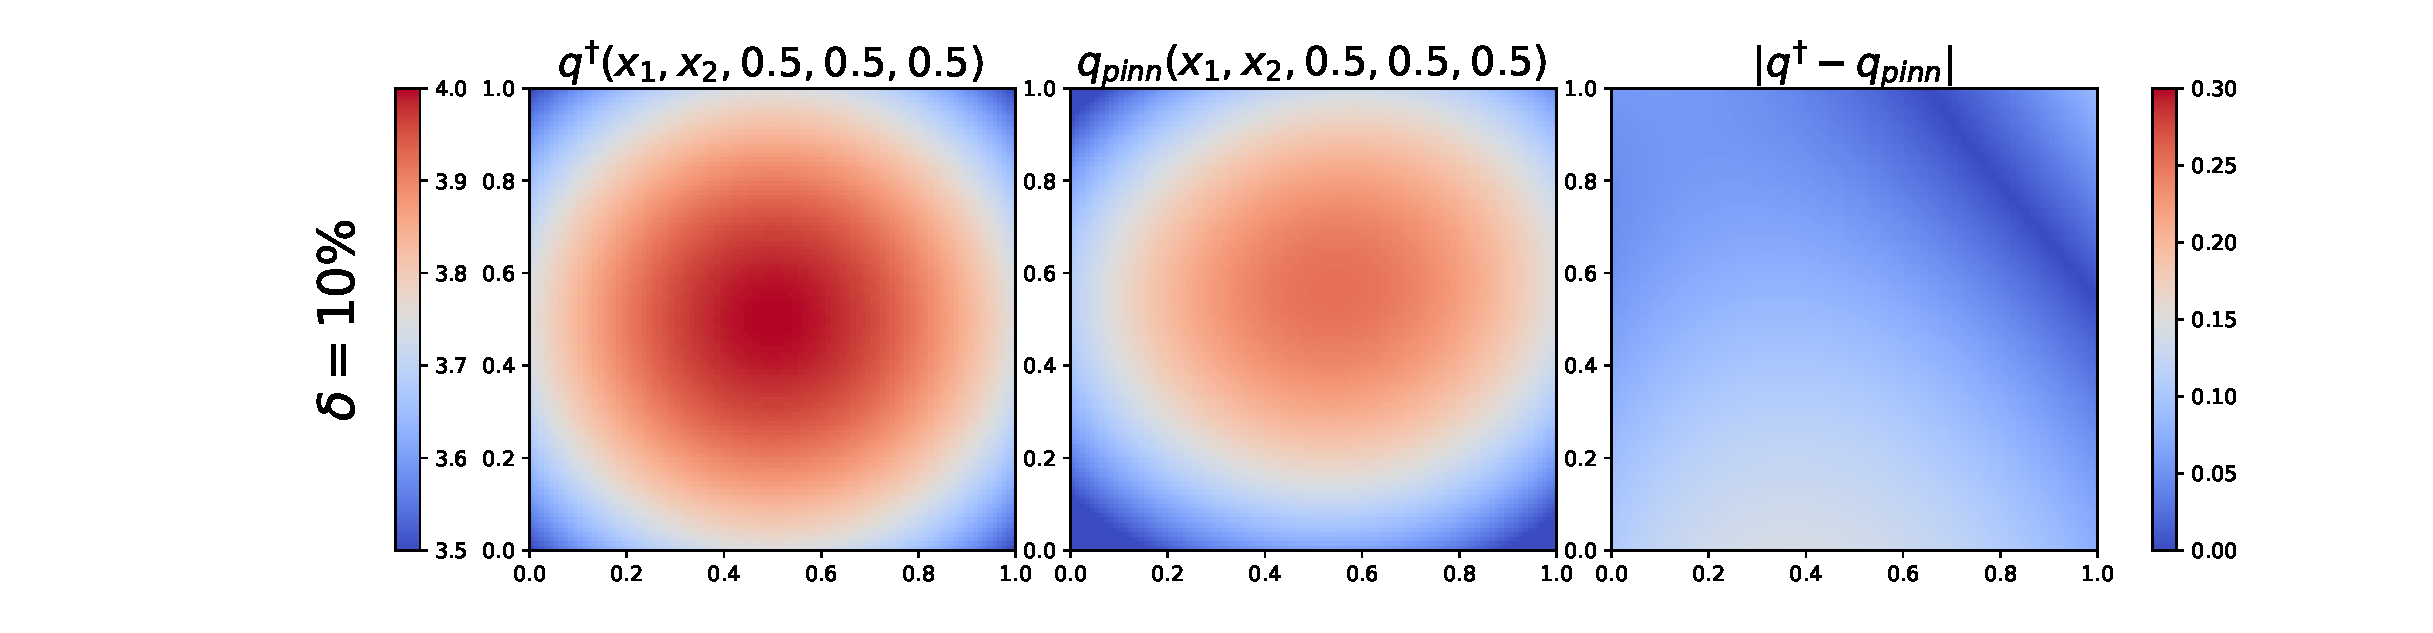
\includegraphics[width=\textwidth]{figures3/ex_5_10.eps}\par
% \caption{算例 \ref{example:highdim} 在切片 $x_3=x_4=x_5=0.5$ 上的真实解与 Tikhonov-PINNs 解。第一行对应 $\delta=0$ 的情况，而第二行展示了 $\delta=10\%$ 的情况。}
% \label{fig:example:highdim}
% \end{figure}

% \begin{table}[hbtp]
% \centering
% \caption{算例 \ref{example:highdim} 中恢复的势 $\hat{q}$ 和解 $\hat{u}$ 的相对 $L^{2}$ 误差。}
% \begin{tabular}{crrrr}
% \hline
% 正则化参数 $\lambda$ & $1.0\times 10^{-7}$ & $1.0\times 10^{-8}$ & $1.0\times 10^{-9}$ & $0$ \\
% \hline
% $\text{err}(u_{\text{pinn}})(\delta=0)$ & $1.09\times 10^{-3}$ & $1.14\times 10^{-3}$ & $1.05\times 10^{-3}$ & $1.39\times 10^{-3}$ \\
% $\text{err}(q_{\text{pinn}})(\delta=0)$ & $3.14\times 10^{-2}$ & $3.08\times 10^{-2}$ & \textbf{3.07$\times$ 10$^{-2}$} & $3.09\times 10^{-2}$  \\
% $\text{err}(u_{\text{pinn}})(\delta=10\%)$ & $4.21\times 10^{-3}$ & $4.19\times 10^{-3}$ & $4.19\times 10^{-3}$ & $4.18\times 10^{-3}$  \\
% $\text{err}(q_{\text{pinn}})(\delta=10\%)$ & $4.33\times 10^{-2}$ & $4.25\times 10^{-2}$ & \textbf{4.24$\times$ 10$^{-2}$} & \textbf{4.24$\times$ 10$^{-2}$}  \\
% \hline
% \end{tabular}
% \label{tab:highdim}
% \end{table}

% 在实验中，我们使用了一个包含 4 个隐藏层且宽度为 26 的神经网络。我们在内部采样了 60,000 个点，在边界上采样了 60,000 个点。模型使用 Adam 优化器训练了 50,000 次迭代，学习率为 $10^{-4}$, 权重衰减系数为 $10^{-9}$。

% 算法误差结果总结在表 \ref{tab:highdim} 中。此外，我们对 $x_{3}=x_{4}=x_{5}=0.5$ 处的切片进行了可视化，如图~\ref{fig:example:highdim} 所示。结果表明，Tikhonov-PINNs 在解决这一五维问题时依然有效，能够准确逼近解和潜在的势函数。

\subsection{缓解半收敛现象}\label{sec:semi_converge}
众所周知，半收敛现象经常出现在不适定反问题中 \cite{engl1996regularization}。在优化的早期阶段，迭代解逐渐逼近真实解。然而，随着迭代的进行，数据噪声的放大导致解偏离真实解，从而导致误差增加。正如 Figure~\ref{fig:err_q} 所示，对于算例 5.3，基于有限元的方法的重构误差最初下降，但随后显著上升，特别是在高噪声水平下。相比之下，Tikhonov-PINNs 有效地缓解了这一问题。我们方法的误差随着迭代次数的增加平滑且持续地下降，没有表现出明显的上升。半收敛的存在使得必须使用早停法来获得最优解，这降低了方法的鲁棒性并限制了可达到的精度。相比之下，Tikhonov-PINNs 固有的优势使其对噪声不那么敏感，允许更多的迭代，最终产生更准确的重构结果。

此外，我们也可以使用算例 5.3 来比较计算成本。在求解算例 5.3 的单次迭代中，Tikhonov-PINNs 平均需要 1.91 秒，而基于 FEM 的方法需要 2.04 秒。如图 10 所示，经过 120 次迭代（229.2 秒）后，Tikhonov-PINNs 在约 $10^6$ 个采样点下达到了约 $O(10^{-2})$ 的精度。相比之下，基于 FEM 的方法进行 120 次迭代需要 244.8 秒，达到的精度为 $O(10^{-1})$。这些结果凸显了 Tikhonov-PINNs 在精度和计算效率方面的明显优势，特别是对于不连续问题。

\begin{figure}[htbp]
   \centering
   \setlength{\abovecaptionskip}{10pt}
   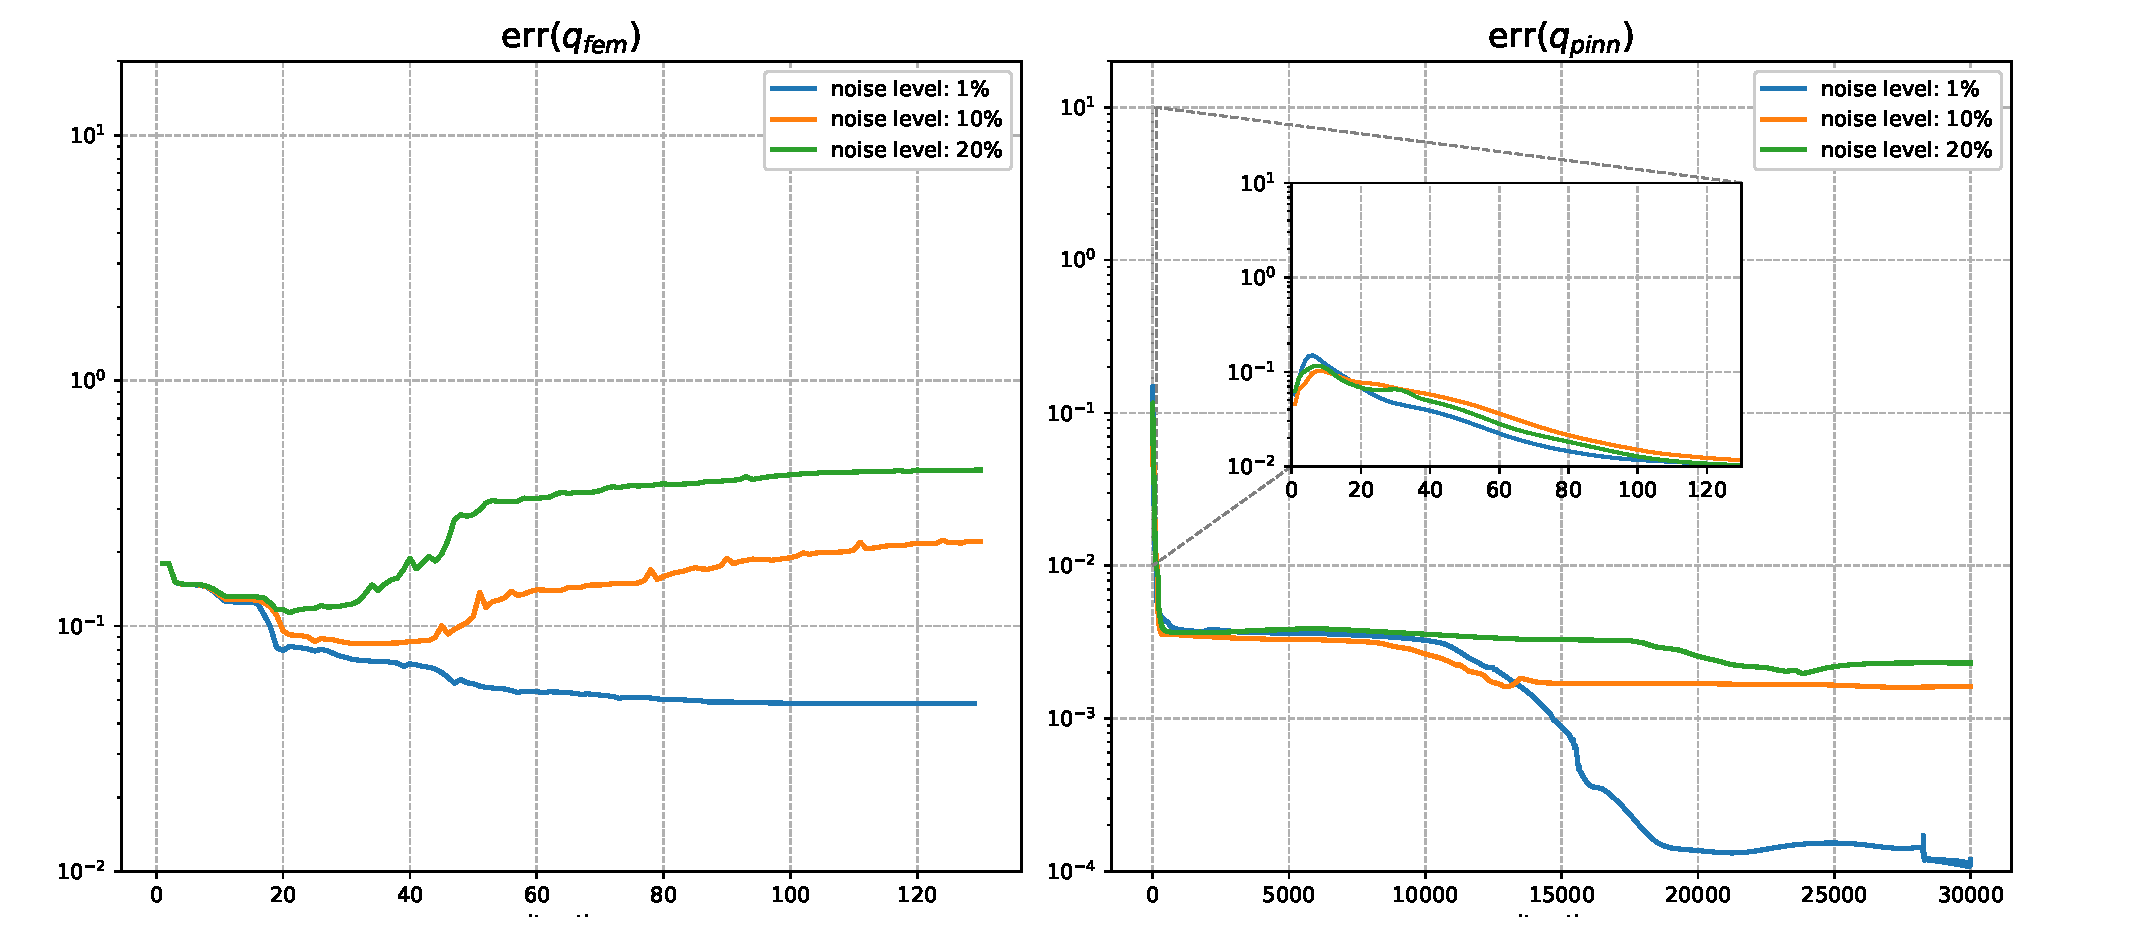
\includegraphics[width=\textwidth]{figures3/err_q.eps}
   \caption{算例~\ref{example:nonsmooth} 中重构势函数 $q$ 的相对 $L^{2}$ 误差随迭代次数变化的曲线。左列显示了有限元方法获得的结果，而右列显示了 Tikhonov-PINNs 获得的结果。}
   \label{fig:err_q}
\end{figure}

% \section{数值实验}\label{sec:numerical}

% 为验证 Tikhonov-PINNs 方法的有效性，我们进行了以下数值实验。所有实验基于 PyTorch 框架，在配备 NVIDIA Tesla V100 GPU 的服务器上完成。

% \subsection{实验设置}

% \textbf{网络结构：} 我们采用深度为 6、宽度为 100 的全连接 ReLU 网络。为保证 $H^2$ 正则性，输出层前添加 ReLU$^2$ 激活函数。

% \textbf{优化器：} 使用 Adam 优化器，初始学习率 $10^{-3}$，每 5000 步衰减为原来的 0.9，总训练步数 40000。

% \textbf{采样策略：} 区域内部采样 $n_{\calI}=10000$ 个点，边界采样 $n_{\calB}=2000$ 个点。测量数据点 $m_{\calI}=5000$，$m_{\calB}=1000$。

% \textbf{超参数：} 惩罚参数 $\mu_1=1000$，$\mu_2=200$，Tikhonov 正则化参数 $\lambda=0.01$。

% \subsection{光滑势函数重构}

% 考虑二维单位正方形区域 $\Omega=[0,1]^2$，传导系数 $\alpha\equiv 1$，源项 $f\equiv 0$，通量 $g\equiv 0$。精确势函数取为：
% \begin{equation*}
% V^\dagger(x) = 2 + \sin(2\pi x_1)\cos(2\pi x_2).
% \end{equation*}

% 图 \ref{fig:eq1_twopeak} 展示了精确势函数、重构势函数及其误差的分布。可以看出，Tikhonov-PINNs 方法能够准确捕捉势函数的光滑变化特征，最大相对误差小于 5\%。

% \begin{figure}[htbp]
%     \centering
%     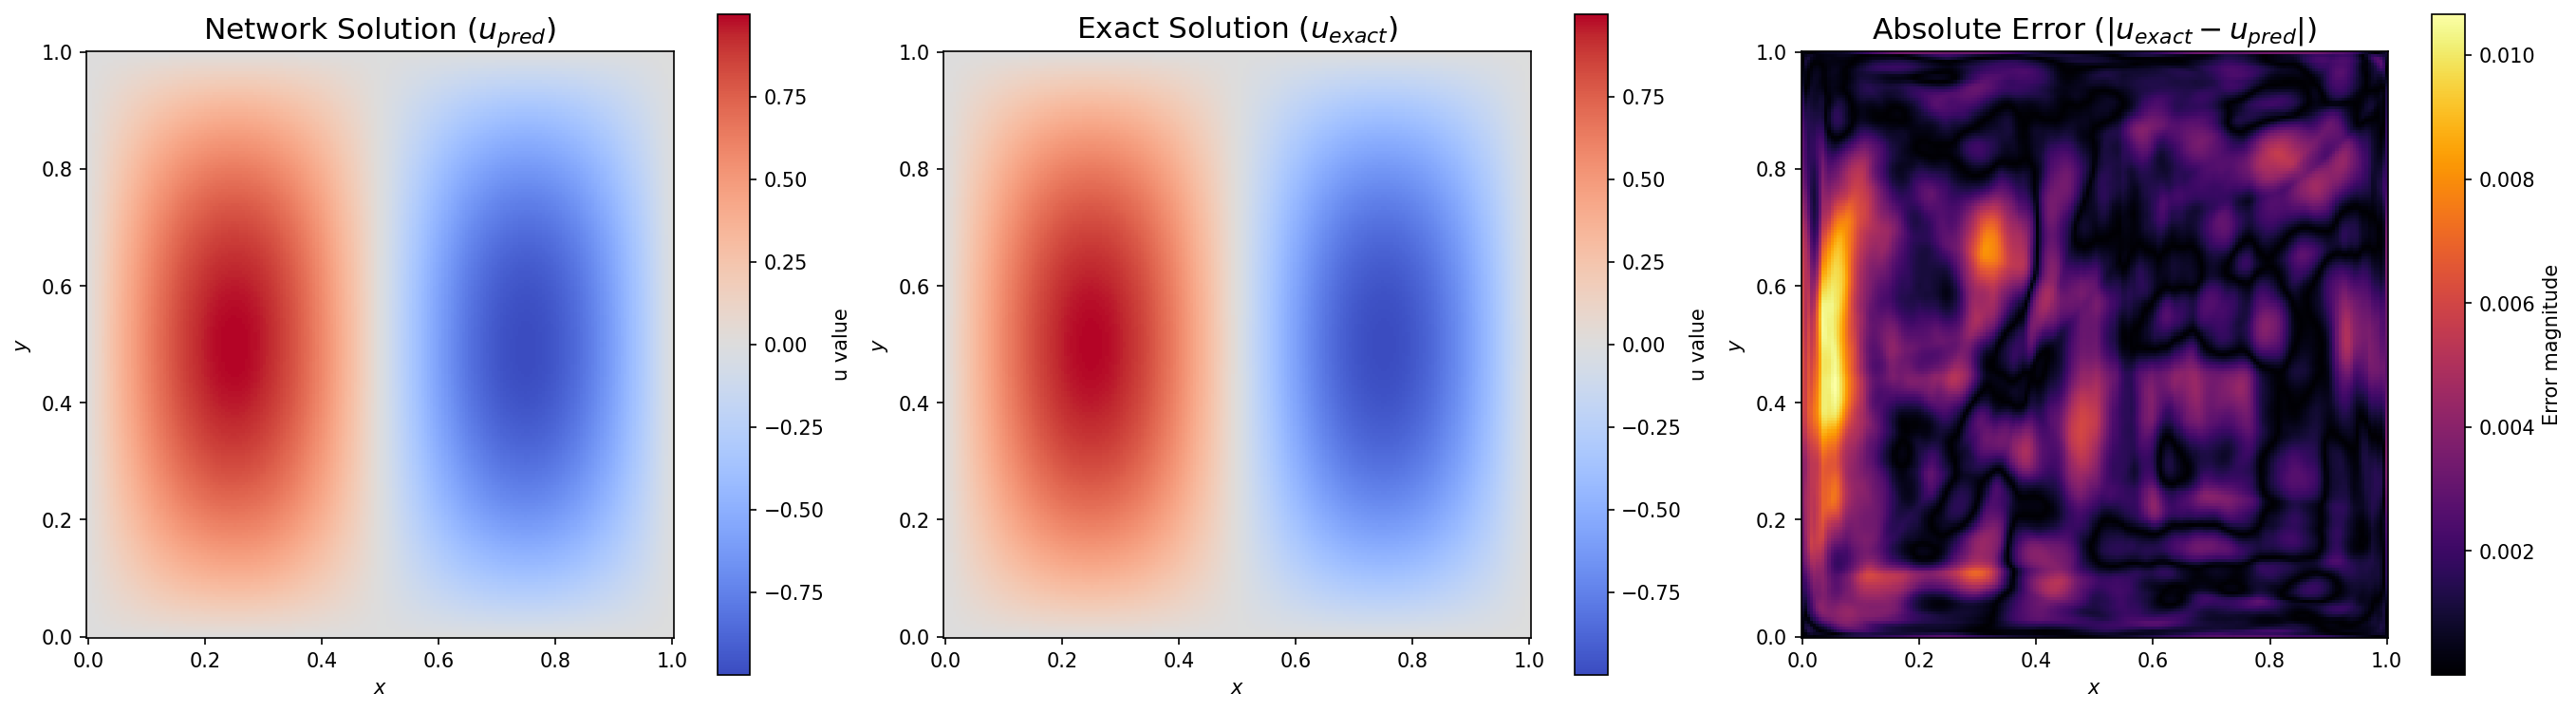
\includegraphics[width=\textwidth]{./figures2/eq1_twopeak_heatmap.png}
%     \caption{光滑势函数重构：精确解、预测解与误差分布}
%     \label{fig:eq1_twopeak}
% \end{figure}

% 图 \ref{fig:eq1_loss} 展示了训练过程中损失函数和验证误差的演化曲线。方法在约 20000 步后达到稳定收敛状态。

% \begin{figure}[htbp]
%     \centering
%     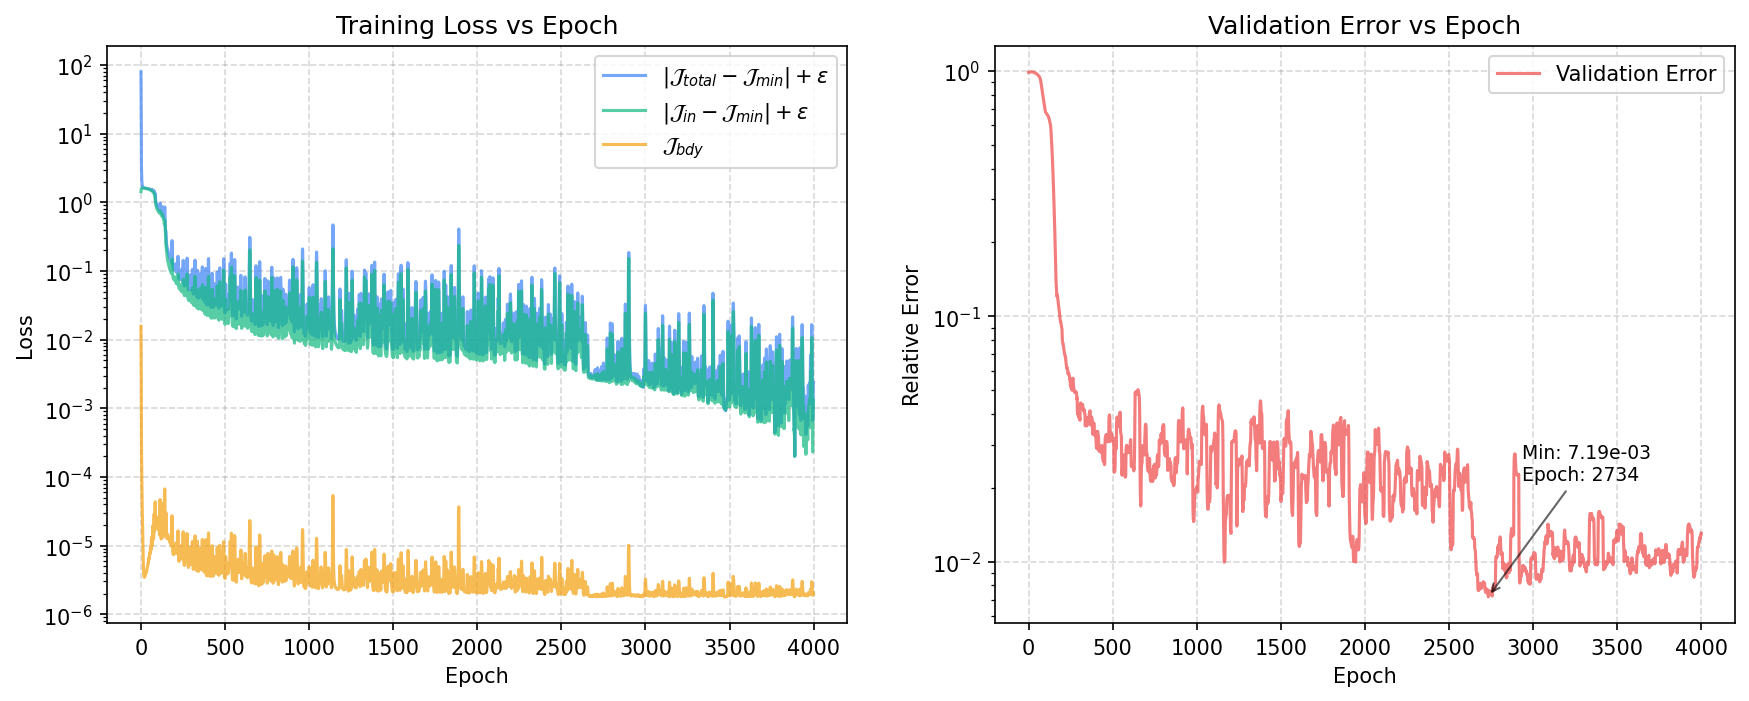
\includegraphics[width=0.9\textwidth]{./figures2/eq1_loss_val_error_curves.png}
%     \caption{光滑势函数重构：训练损失与验证误差曲线}
%     \label{fig:eq1_loss}
% \end{figure}

% \subsection{不连续势函数重构}

% 为测试方法对非光滑势函数的适应能力，考虑分段常数势函数：
% \begin{equation*}
% V^\dagger(x) = \begin{cases}
% 3, & \|x - (0.5, 0.5)\|_2 < 0.3, \\
% 1, & \text{其他}.
% \end{cases}
% \end{equation*}

% 图 \ref{fig:eq2_nondiff} 展示了重构结果。尽管势函数在间断处不可导，Tikhonov-PINNs 方法仍能较准确地捕捉势函数的整体分布，间断边界处的相对误差约为 10\%。

% \begin{figure}[htbp]
%     \centering
%     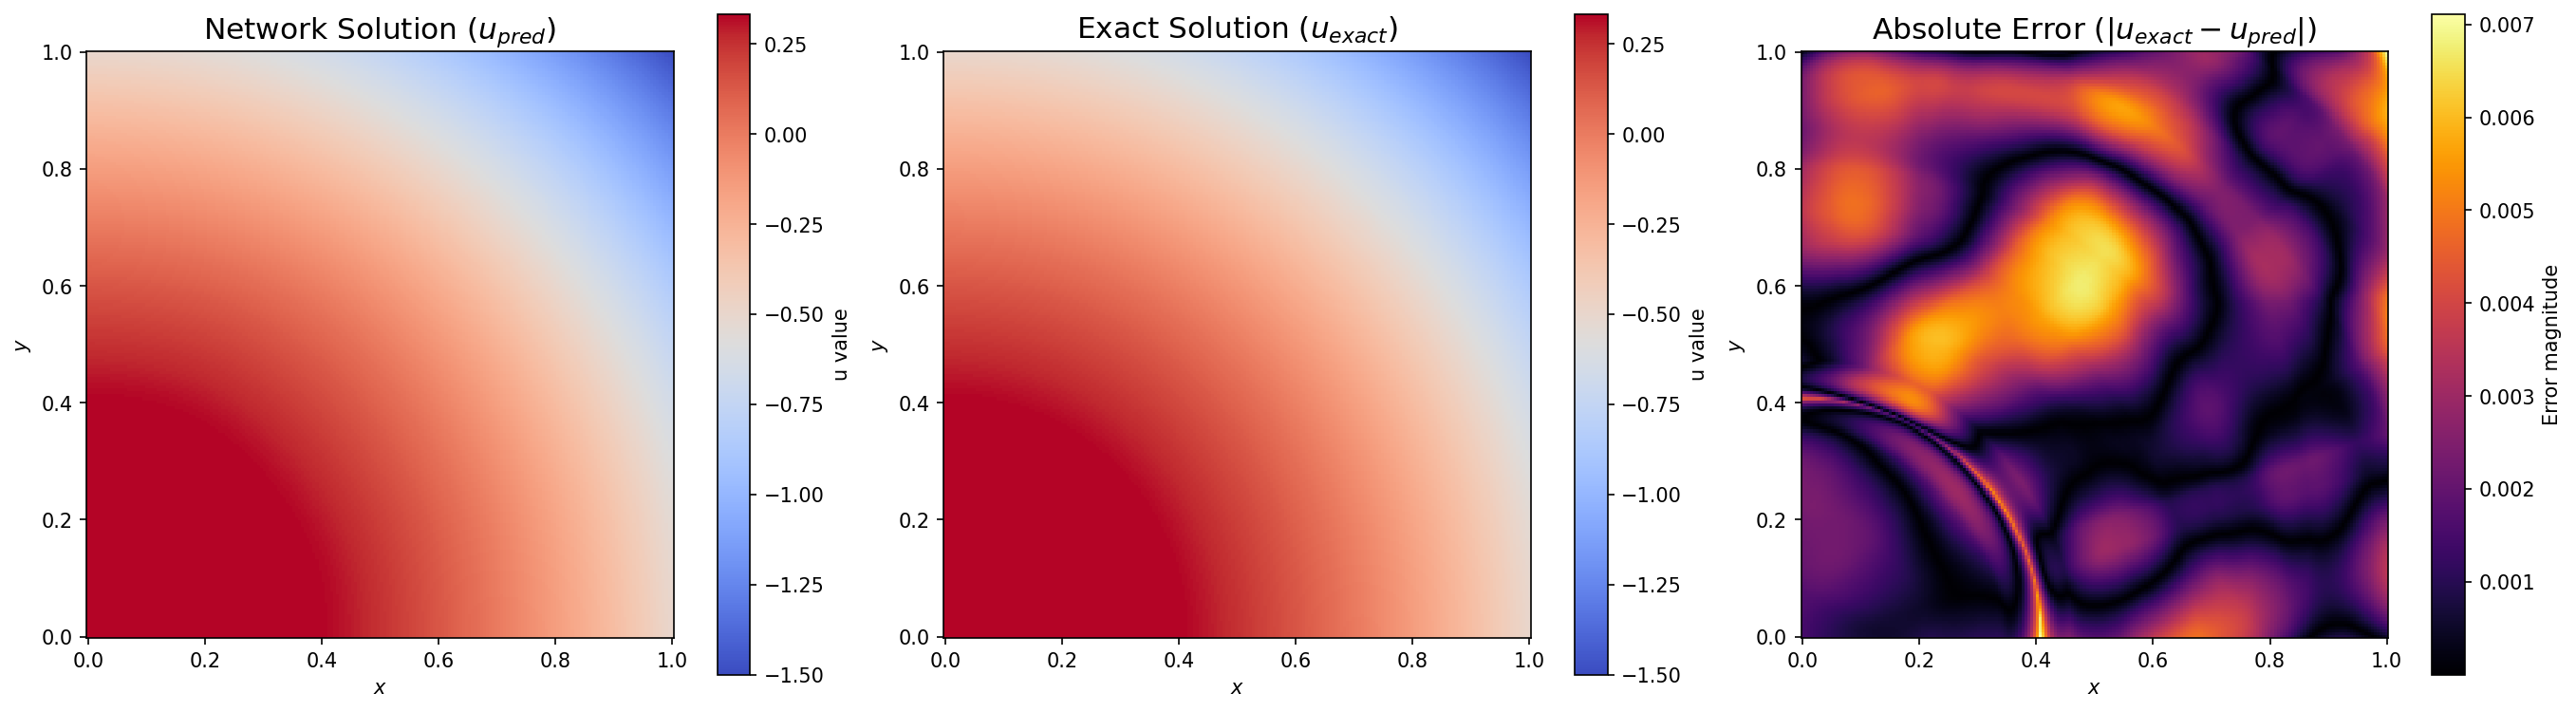
\includegraphics[width=\textwidth]{./figures2/eq2_nondiff_heatmap.png}
%     \caption{不连续势函数重构：精确解、预测解与误差分布}
%     \label{fig:eq2_nondiff}
% \end{figure}

% \subsection{不同噪声水平下的鲁棒性}

% 我们测试了方法在不同噪声水平 $\delta$ 下的表现。表 \ref{tab:noise} 列出了不同噪声水平下的相对误差。结果显示，随着噪声水平的降低，重构精度单调提高，验证了方法的鲁棒性。

% \begin{table}[htbp]
% \centering
% \caption{不同噪声水平下的重构误差}
% \label{tab:noise}
% \begin{tabular}{c|ccccc}
% \hline
% 噪声水平 $\delta$ & 0.1 & 0.05 & 0.02 & 0.01 & 0.005 \\
% \hline
% 相对误差 (\%) & 18.3 & 12.1 & 6.5 & 3.8 & 2.1 \\
% \hline
% \end{tabular}
% \end{table}


\section{附录}\label{sec:appendix}
